% Generated by `python -m experiments.experiment_1.appendix_captions` -- do not edit by hand.
% Needs \usepackage{graphicx,subcaption}; paths are relative to outputs/finals/experiment-1/.
% Mixed-predictor case and benchmark ensembles, CogFormer only; panel encodings refer to fig:app1-ddm-intercept-only-cf
% (outputs/finals/experiment-1a/captions.tex).

% ── mixed-predictor case ──

\begin{figure}[p]
  \centering
  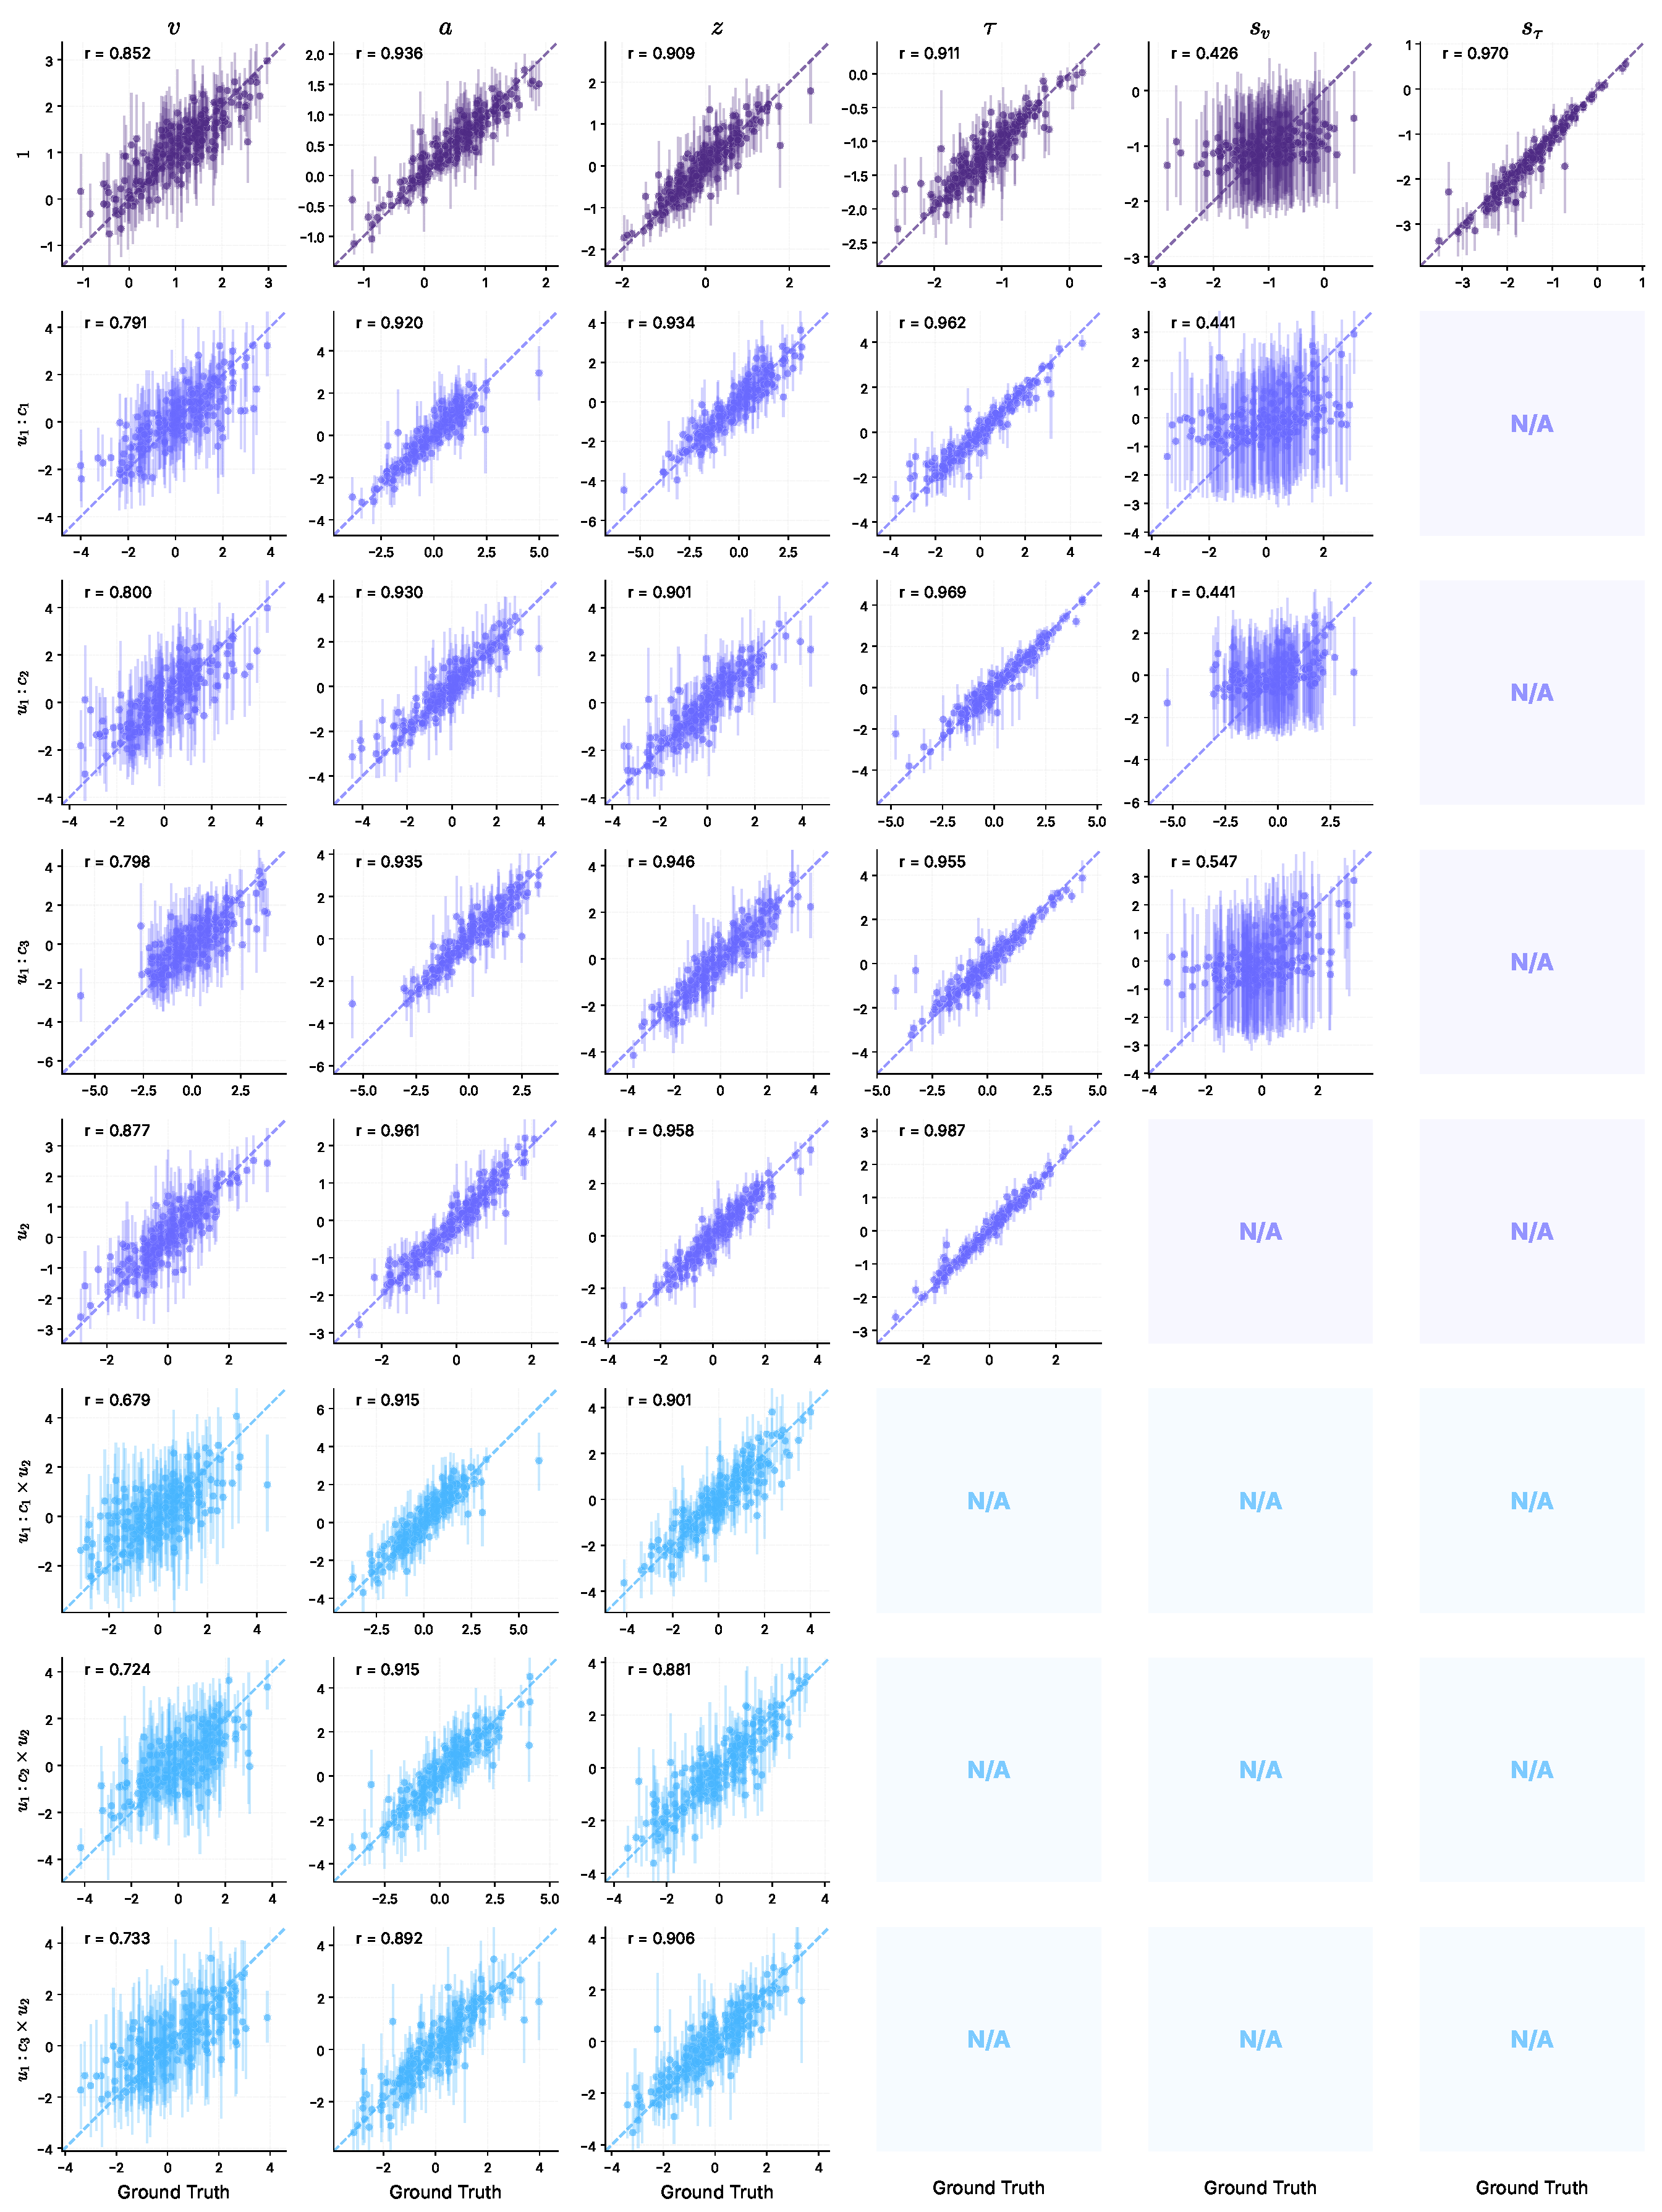
\includegraphics[width=\textwidth,height=0.82\textheight,keepaspectratio]{per_case/ddm/mixed_predictor/recovery.pdf}
  \caption{\textbf{Parameter recovery, DDM, \emph{mixed-predictor} design (CogFormer).} The design combines a categorical and a continuous regressor: $u_1$ has 4 levels and is dummy-coded against a reference level, giving one row per contrast ($u_1{:}c_1$ to $u_1{:}c_3$); $u_2$ is continuous; and the rows $u_1{:}c_k \times u_2$ are their interaction, one per contrast. $v$, $a$, $z$, $\tau$ and $s_v$ carry effects of $u_1$; $v$, $a$, $z$ and $\tau$ carry slopes on $u_2$; $v$, $a$ and $z$ carry the interaction (34 coefficients shown). No BayesFlow baseline was trained on this design, so only CogFormer is shown, on 200 datasets (500 trials each) simulated for it, with 200 posterior draws per dataset. Encoding as in panel (a) of Figure~\ref{fig:app1-ddm-intercept-only-cf}; the contamination probability $\pi$ is not shown. Figures~\ref{fig:app1-ddm-mixed-predictor-ecdf}--\ref{fig:app1-cdm-mixed-predictor-metrics} show the remaining diagnostics of this design and the other two families in the same way.}
  \label{fig:app1-ddm-mixed-predictor-recovery}
\end{figure}

\begin{figure}[p]
  \centering
  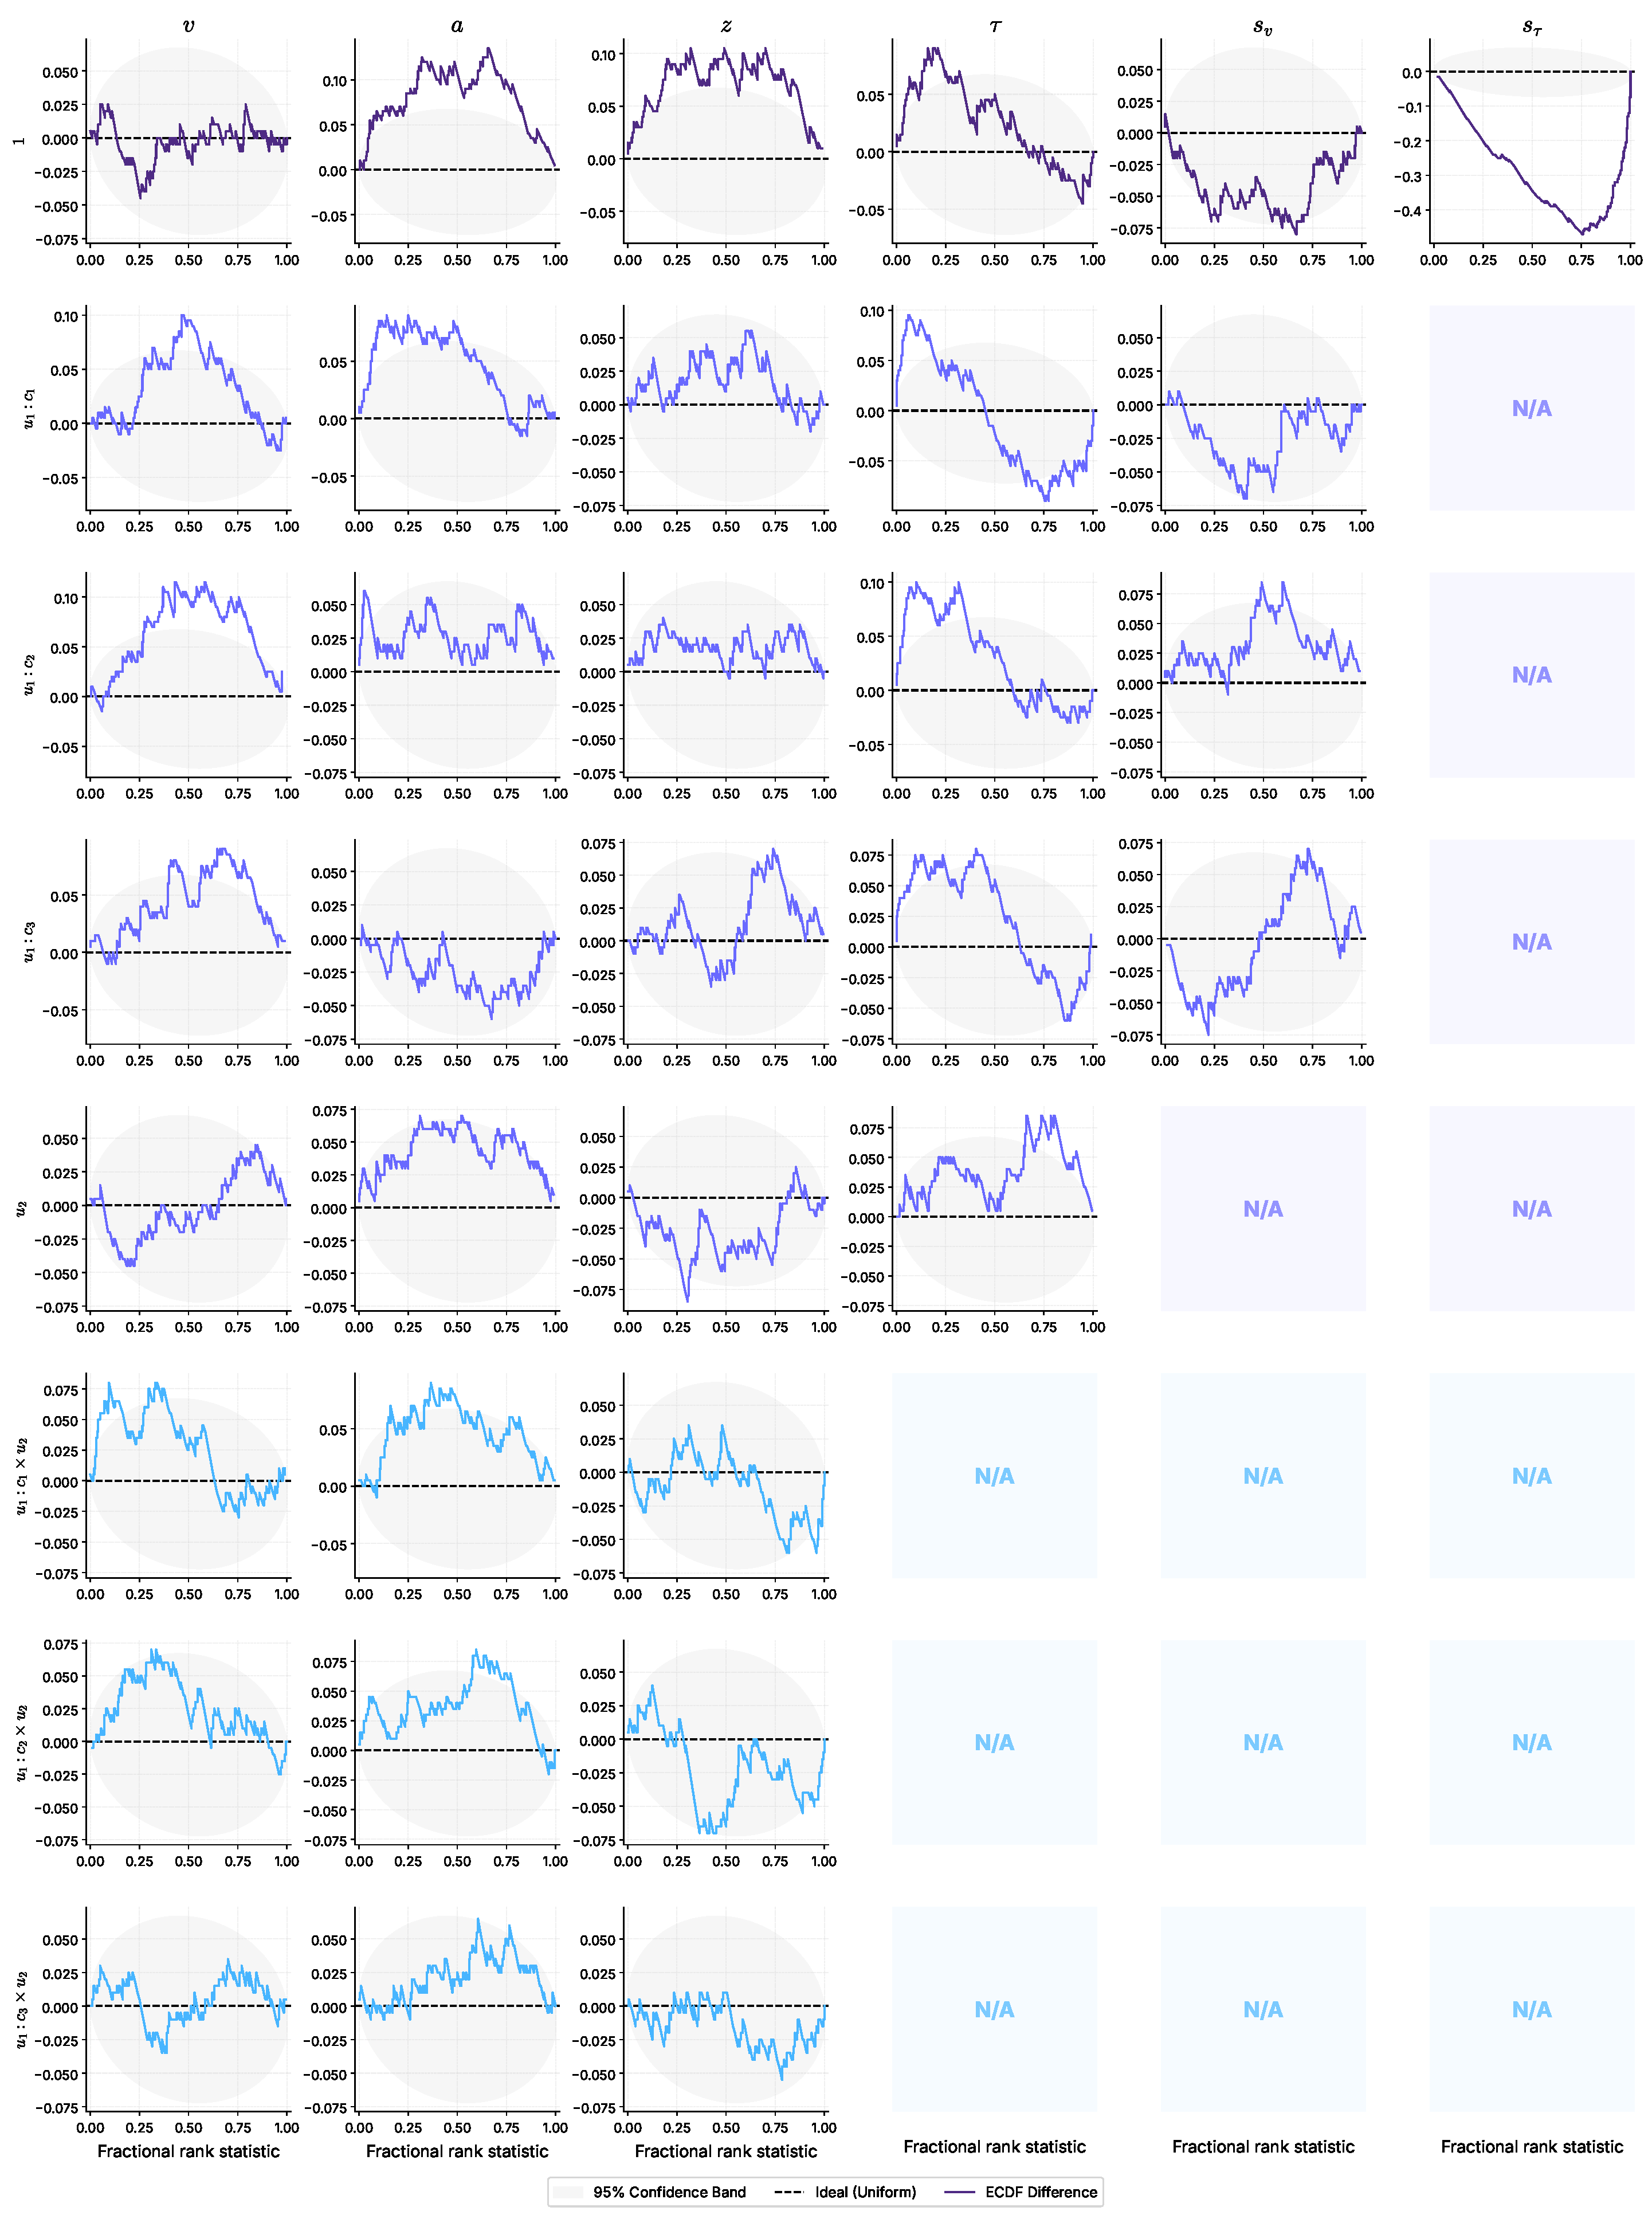
\includegraphics[width=\textwidth,height=0.82\textheight,keepaspectratio]{per_case/ddm/mixed_predictor/ecdf.pdf}
  \caption{\textbf{Simulation-based calibration, DDM, \emph{mixed-predictor} design (CogFormer).} $v$, $a$, $z$, $\tau$ and $s_v$ carry effects of $u_1$; $v$, $a$, $z$ and $\tau$ carry slopes on $u_2$; $v$, $a$ and $z$ carry the interaction (34 coefficients shown). Design as in Figure~\ref{fig:app1-ddm-mixed-predictor-recovery}; encoding as in panel (b) of Figure~\ref{fig:app1-ddm-intercept-only-cf}.}
  \label{fig:app1-ddm-mixed-predictor-ecdf}
\end{figure}

\begin{figure}[p]
  \centering
  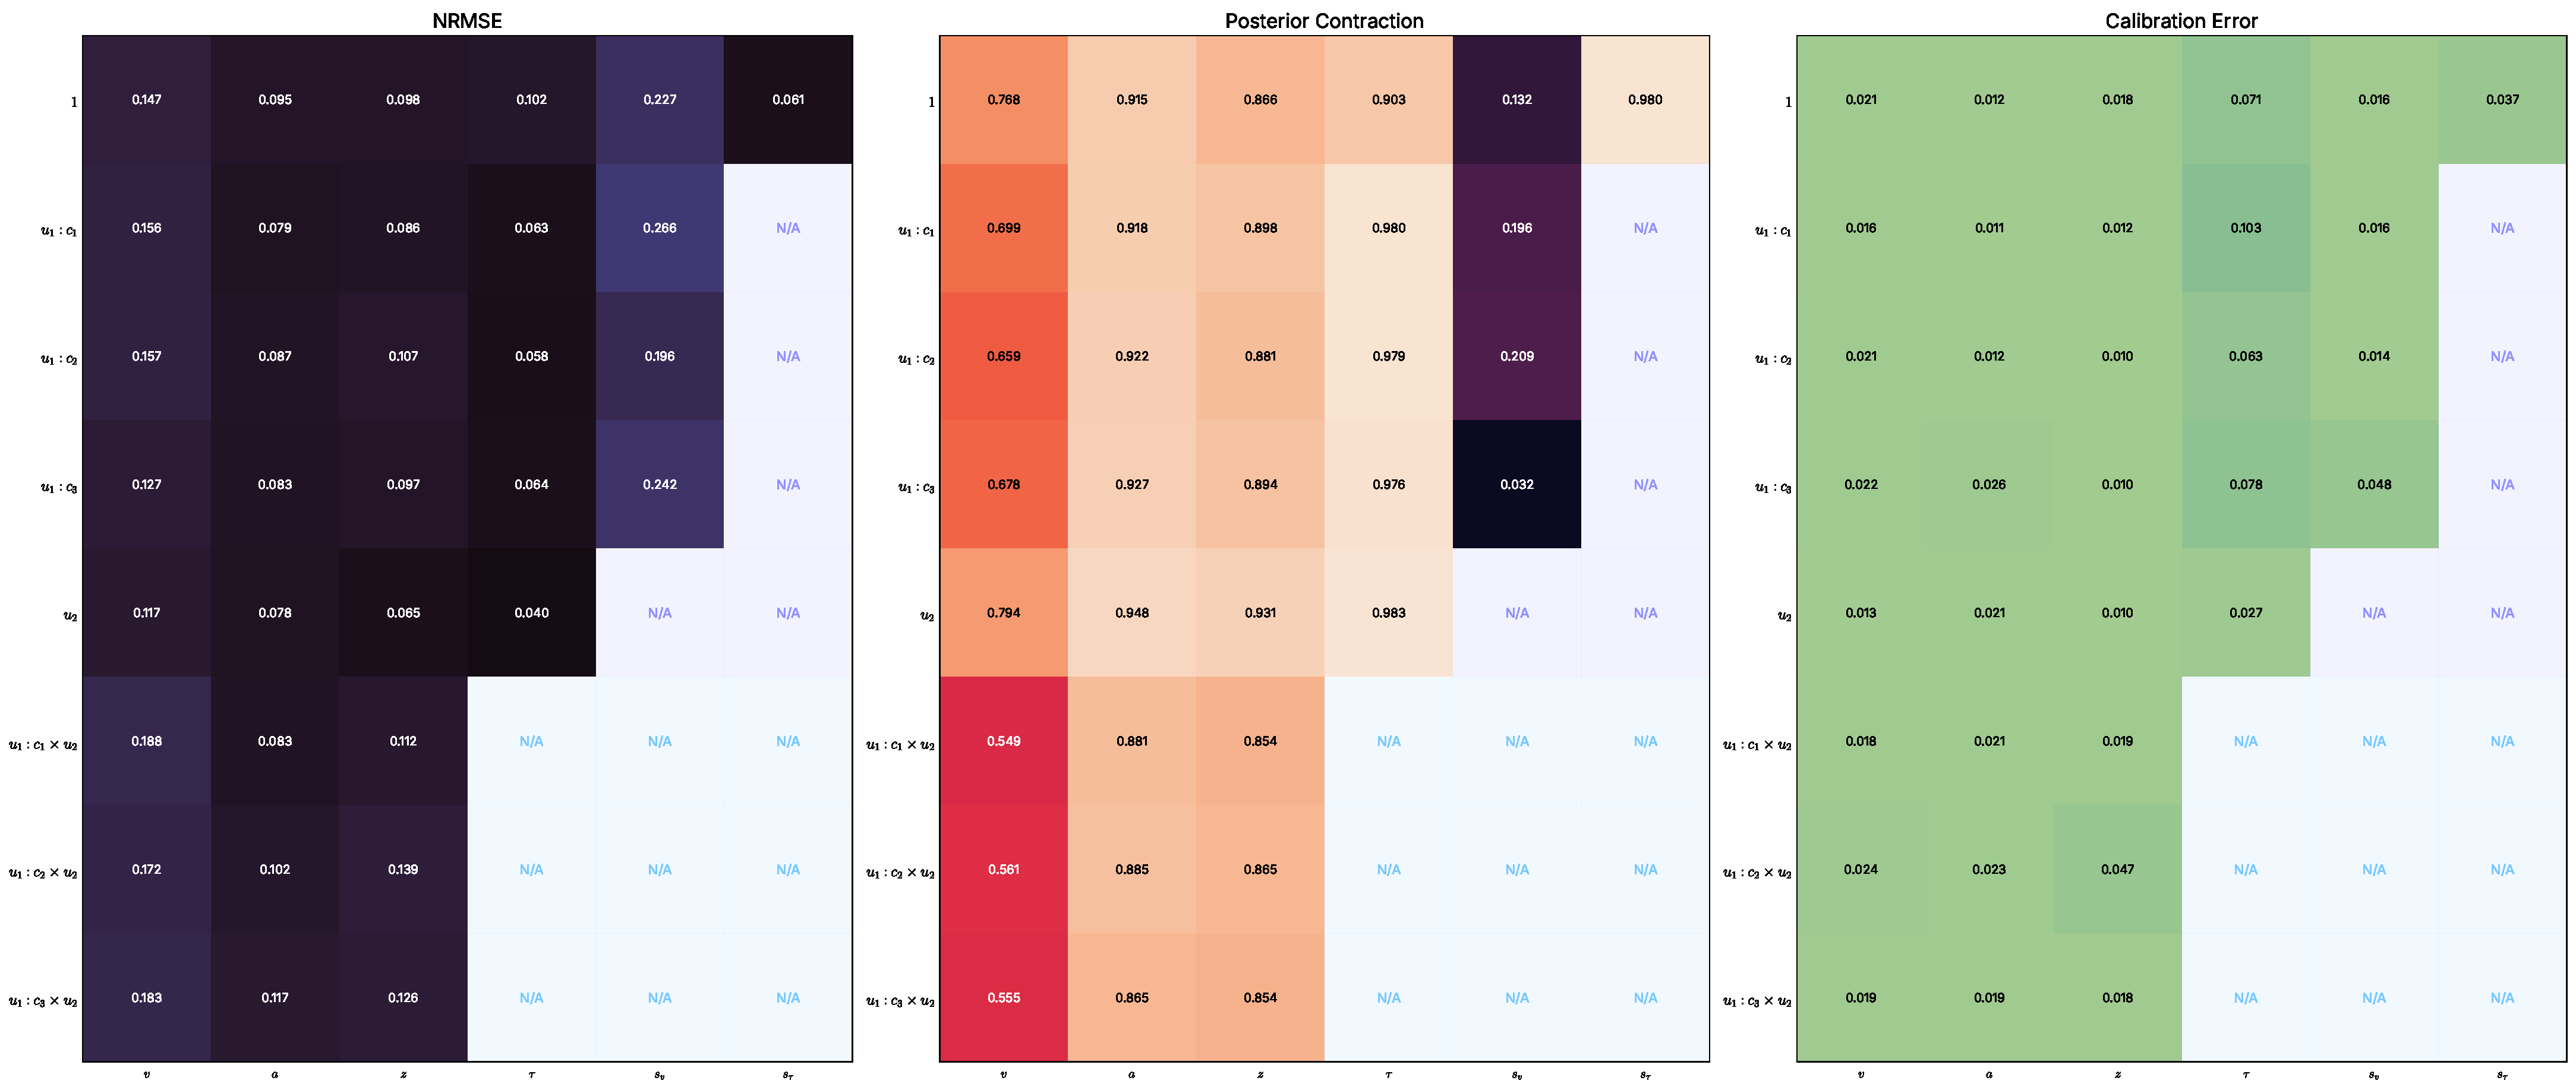
\includegraphics[width=\textwidth,height=0.82\textheight,keepaspectratio]{per_case/ddm/mixed_predictor/metrics.pdf}
  \caption{\textbf{Summary metrics, DDM, \emph{mixed-predictor} design (CogFormer).} $v$, $a$, $z$, $\tau$ and $s_v$ carry effects of $u_1$; $v$, $a$, $z$ and $\tau$ carry slopes on $u_2$; $v$, $a$ and $z$ carry the interaction (34 coefficients shown). Design as in Figure~\ref{fig:app1-ddm-mixed-predictor-recovery}; encoding as in panel (c) of Figure~\ref{fig:app1-ddm-intercept-only-cf}.}
  \label{fig:app1-ddm-mixed-predictor-metrics}
\end{figure}

\begin{figure}[p]
  \centering
  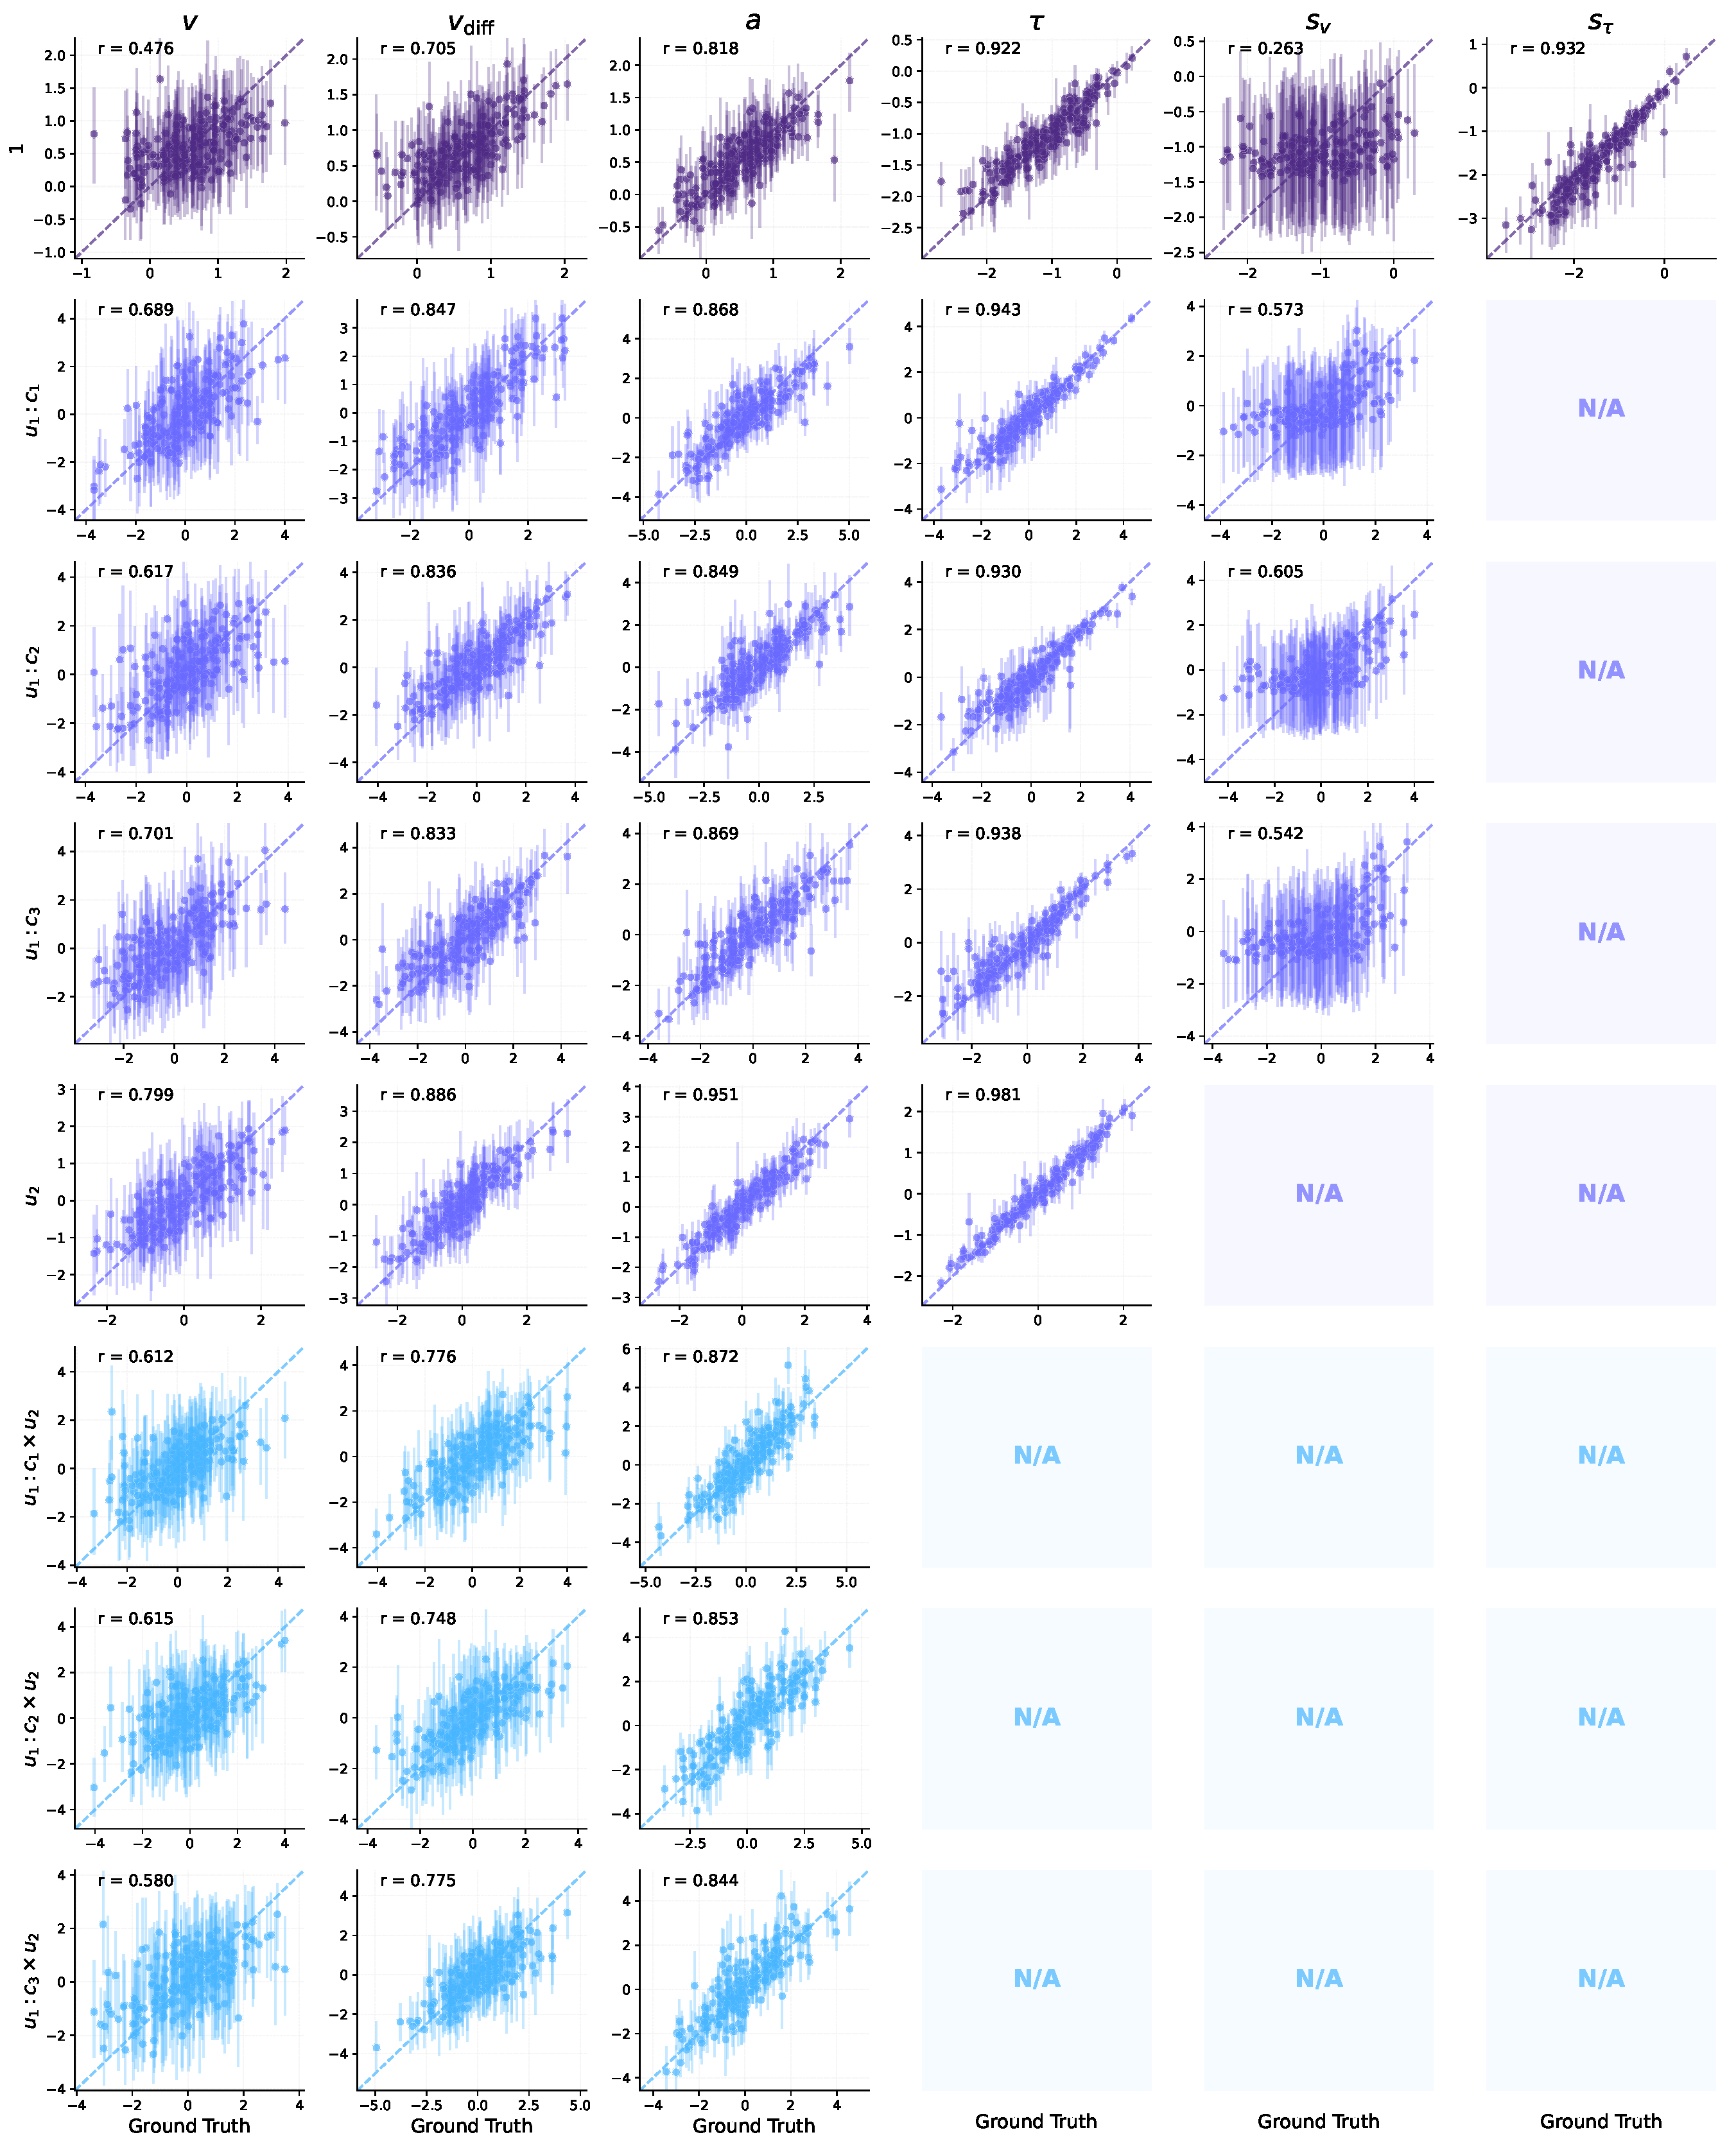
\includegraphics[width=\textwidth,height=0.82\textheight,keepaspectratio]{per_case/rdm/mixed_predictor/recovery.pdf}
  \caption{\textbf{Parameter recovery, RDM, \emph{mixed-predictor} design (CogFormer).} $v$, $v_{\mathrm{diff}}$, $a$, $\tau$ and $s_v$ carry effects of $u_1$; $v$, $v_{\mathrm{diff}}$, $a$ and $\tau$ carry slopes on $u_2$; $v$, $v_{\mathrm{diff}}$ and $a$ carry the interaction (34 coefficients shown). Design as in Figure~\ref{fig:app1-ddm-mixed-predictor-recovery}; encoding as in panel (a) of Figure~\ref{fig:app1-ddm-intercept-only-cf}.}
  \label{fig:app1-rdm-mixed-predictor-recovery}
\end{figure}

\begin{figure}[p]
  \centering
  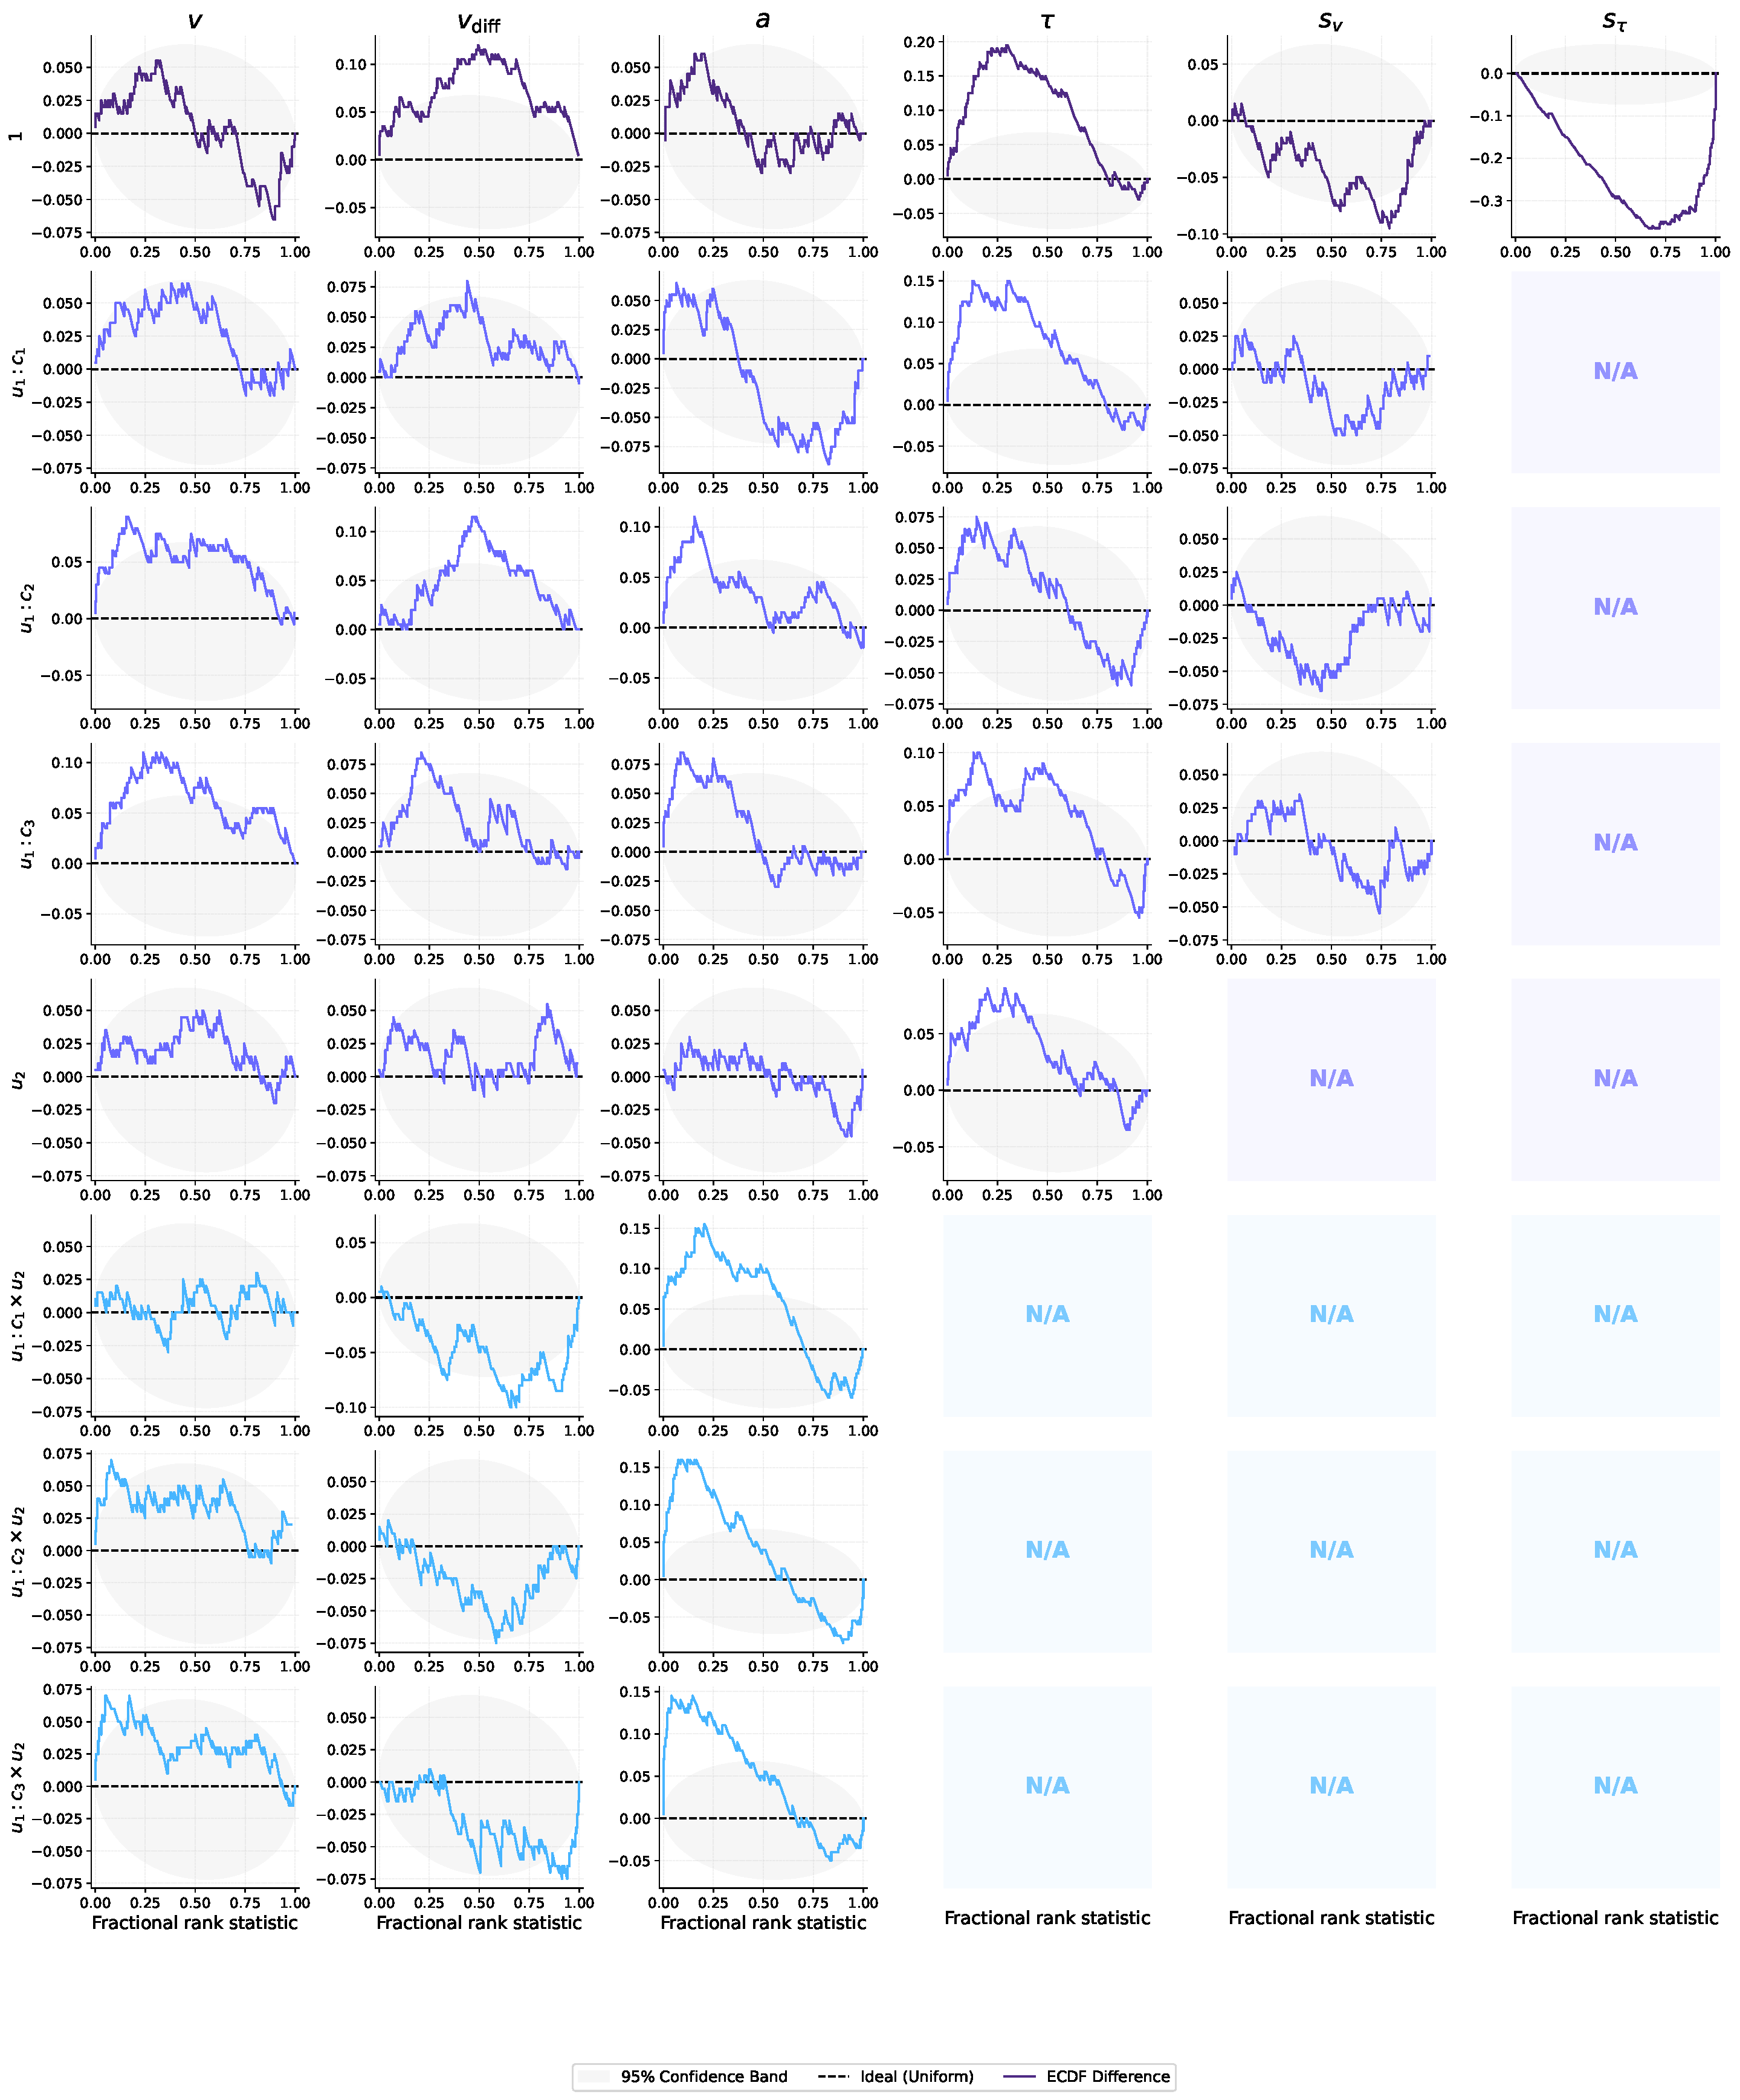
\includegraphics[width=\textwidth,height=0.82\textheight,keepaspectratio]{per_case/rdm/mixed_predictor/ecdf.pdf}
  \caption{\textbf{Simulation-based calibration, RDM, \emph{mixed-predictor} design (CogFormer).} $v$, $v_{\mathrm{diff}}$, $a$, $\tau$ and $s_v$ carry effects of $u_1$; $v$, $v_{\mathrm{diff}}$, $a$ and $\tau$ carry slopes on $u_2$; $v$, $v_{\mathrm{diff}}$ and $a$ carry the interaction (34 coefficients shown). Design as in Figure~\ref{fig:app1-ddm-mixed-predictor-recovery}; encoding as in panel (b) of Figure~\ref{fig:app1-ddm-intercept-only-cf}.}
  \label{fig:app1-rdm-mixed-predictor-ecdf}
\end{figure}

\begin{figure}[p]
  \centering
  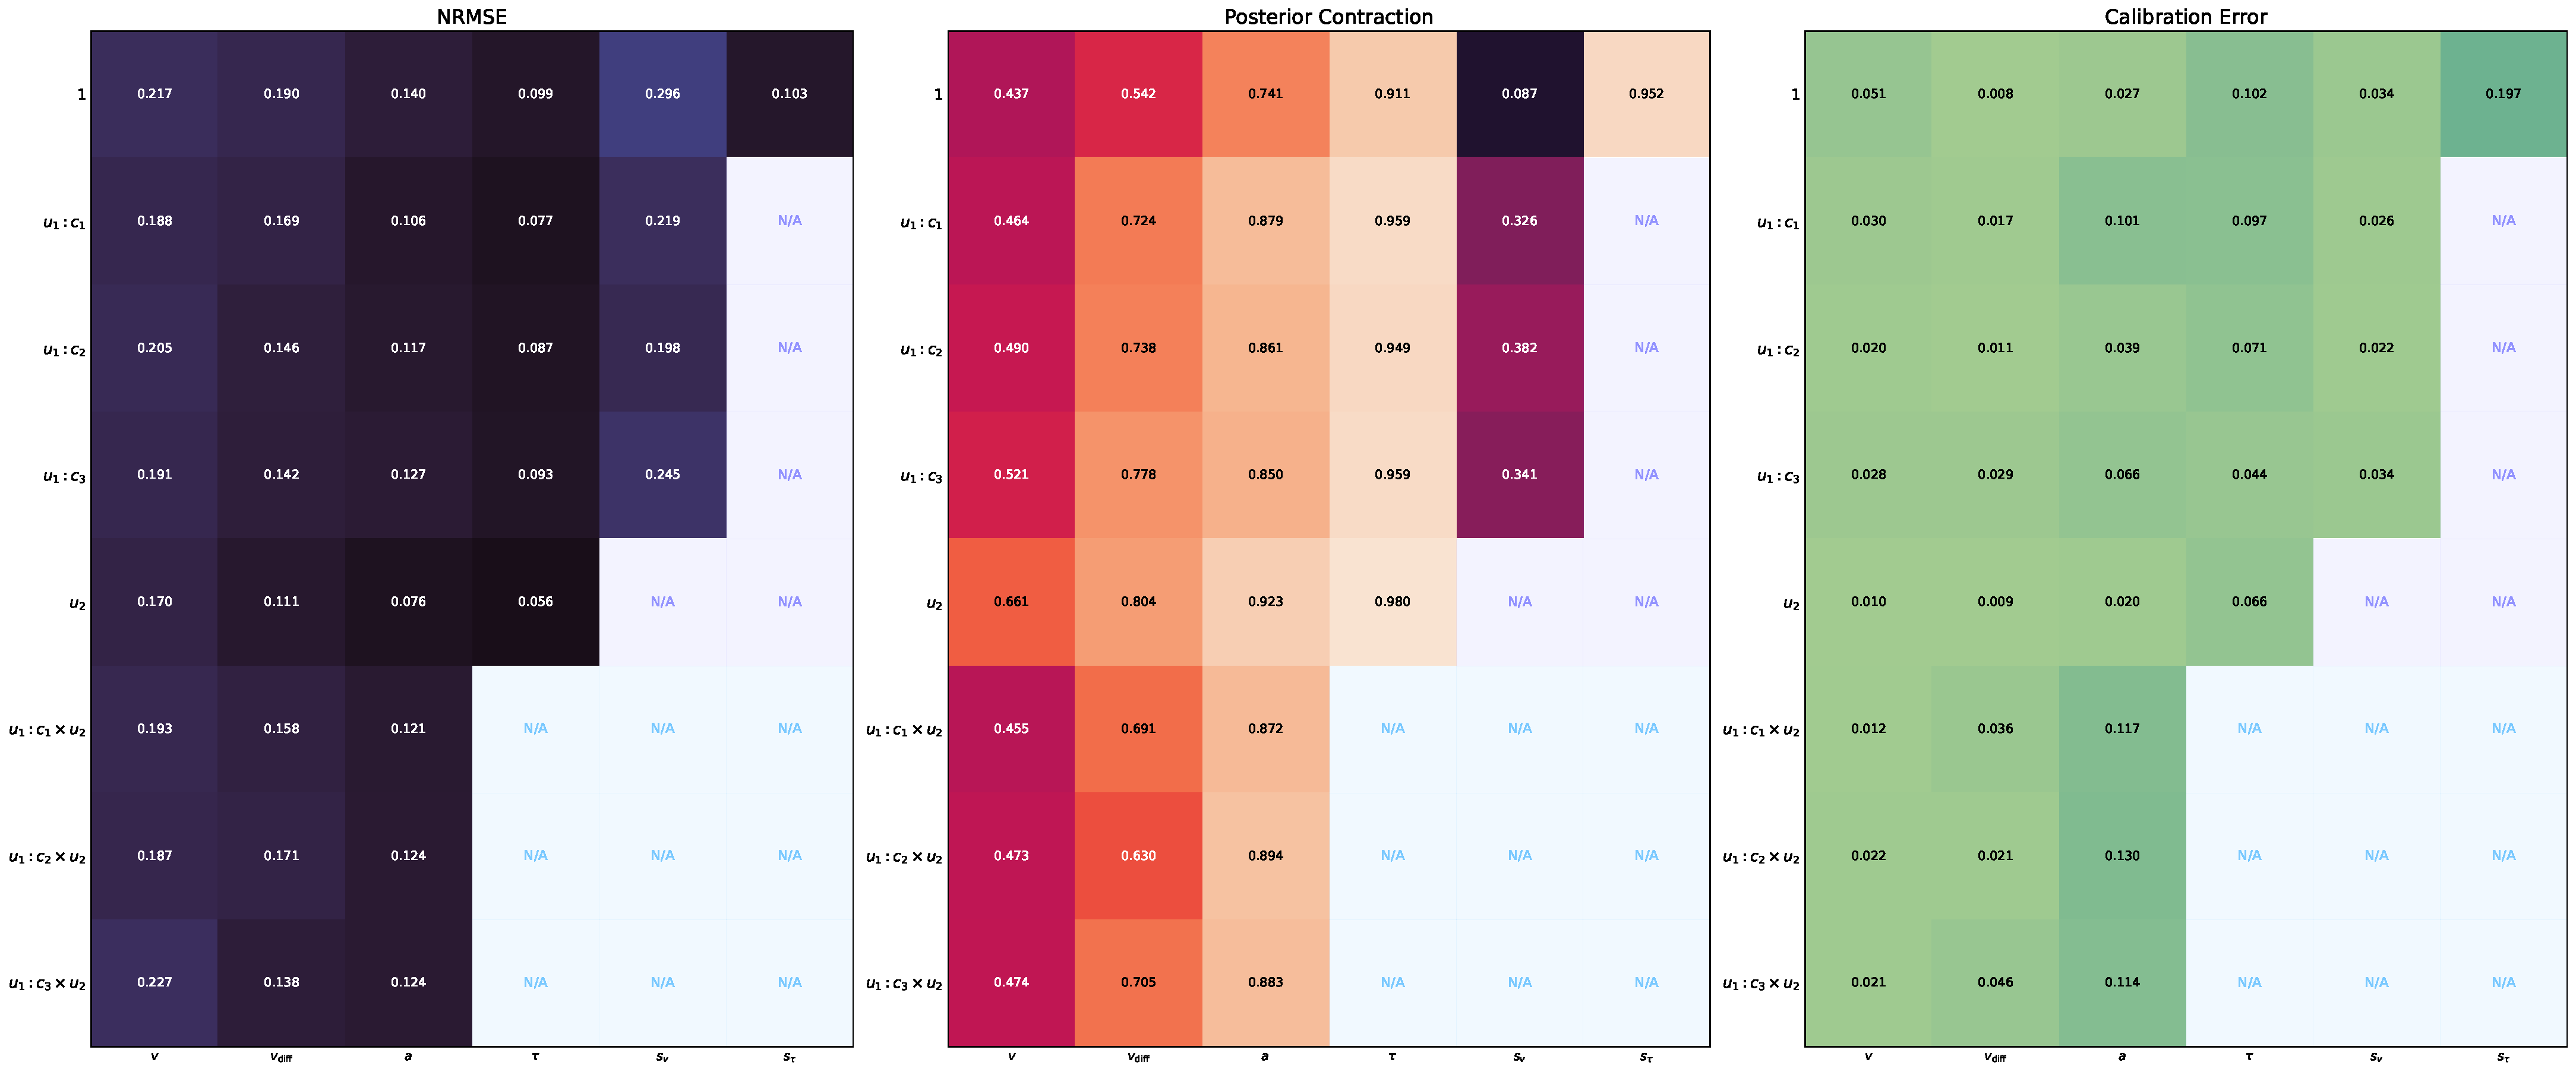
\includegraphics[width=\textwidth,height=0.82\textheight,keepaspectratio]{per_case/rdm/mixed_predictor/metrics.pdf}
  \caption{\textbf{Summary metrics, RDM, \emph{mixed-predictor} design (CogFormer).} $v$, $v_{\mathrm{diff}}$, $a$, $\tau$ and $s_v$ carry effects of $u_1$; $v$, $v_{\mathrm{diff}}$, $a$ and $\tau$ carry slopes on $u_2$; $v$, $v_{\mathrm{diff}}$ and $a$ carry the interaction (34 coefficients shown). Design as in Figure~\ref{fig:app1-ddm-mixed-predictor-recovery}; encoding as in panel (c) of Figure~\ref{fig:app1-ddm-intercept-only-cf}.}
  \label{fig:app1-rdm-mixed-predictor-metrics}
\end{figure}

\begin{figure}[p]
  \centering
  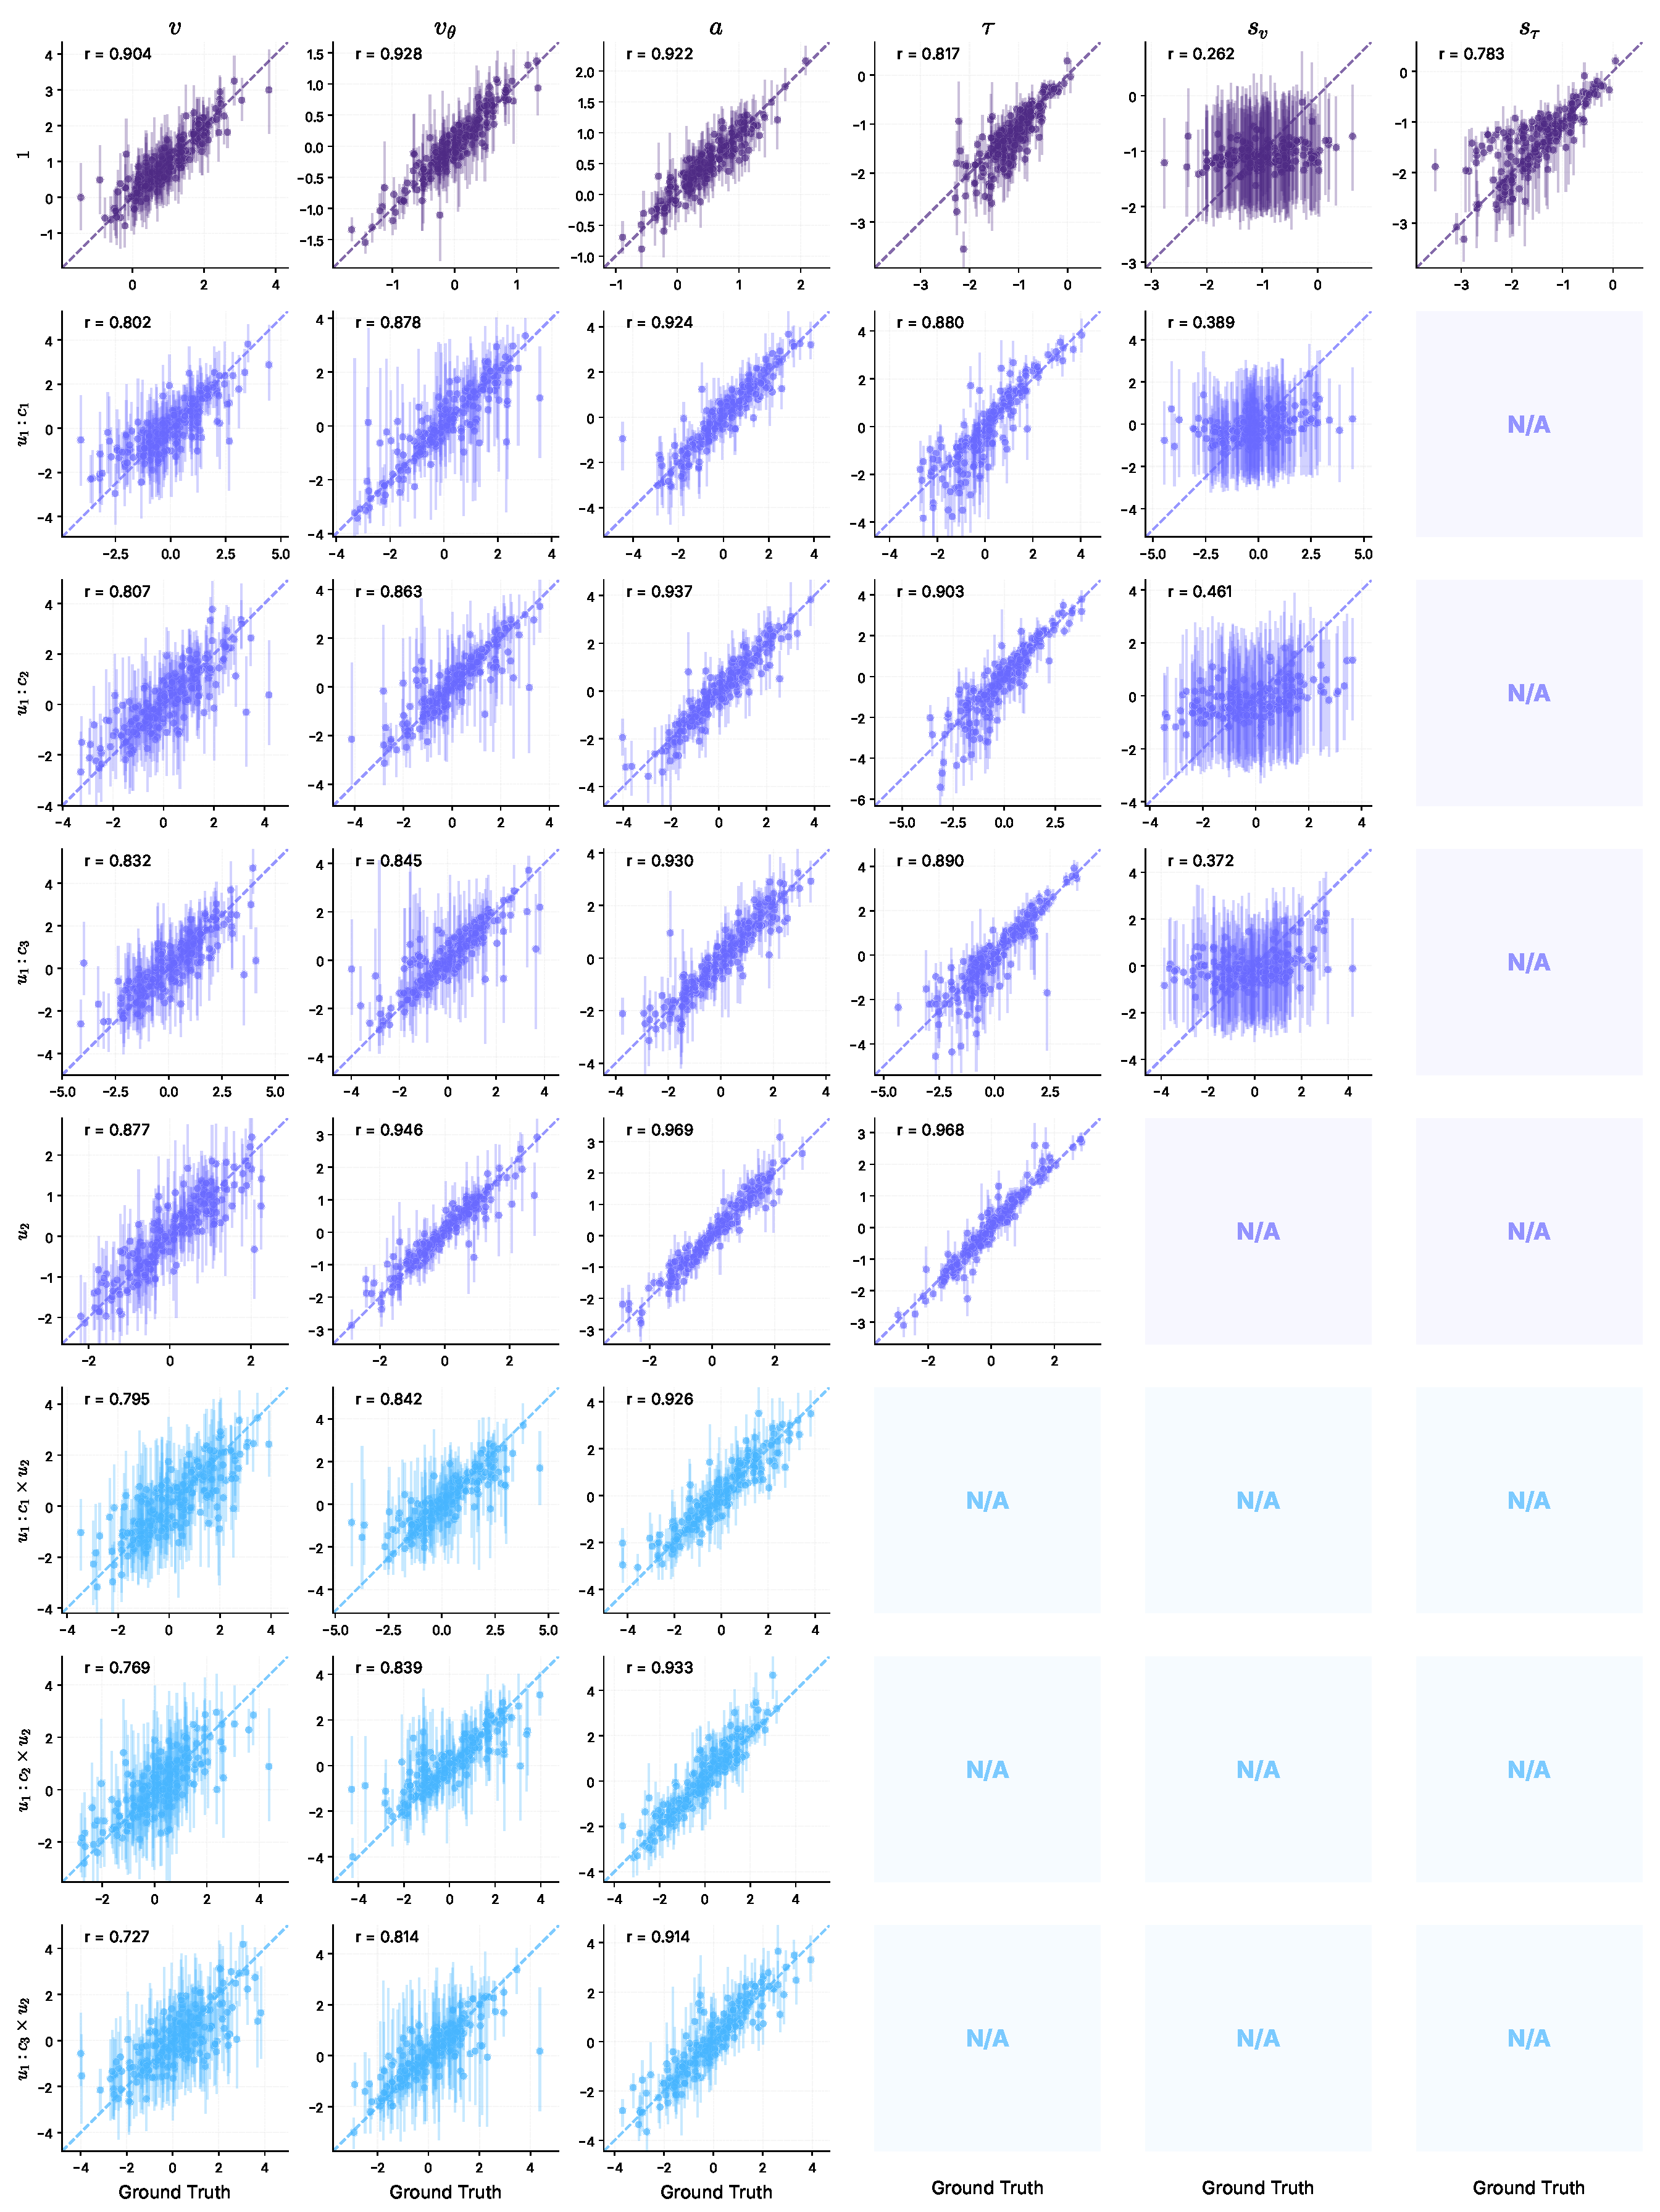
\includegraphics[width=\textwidth,height=0.82\textheight,keepaspectratio]{per_case/cdm/mixed_predictor/recovery.pdf}
  \caption{\textbf{Parameter recovery, CDM, \emph{mixed-predictor} design (CogFormer).} $v$, $v_\theta$, $a$, $\tau$ and $s_v$ carry effects of $u_1$; $v$, $v_\theta$, $a$ and $\tau$ carry slopes on $u_2$; $v$, $v_\theta$ and $a$ carry the interaction (34 coefficients shown). Design as in Figure~\ref{fig:app1-ddm-mixed-predictor-recovery}; encoding as in panel (a) of Figure~\ref{fig:app1-ddm-intercept-only-cf}.}
  \label{fig:app1-cdm-mixed-predictor-recovery}
\end{figure}

\begin{figure}[p]
  \centering
  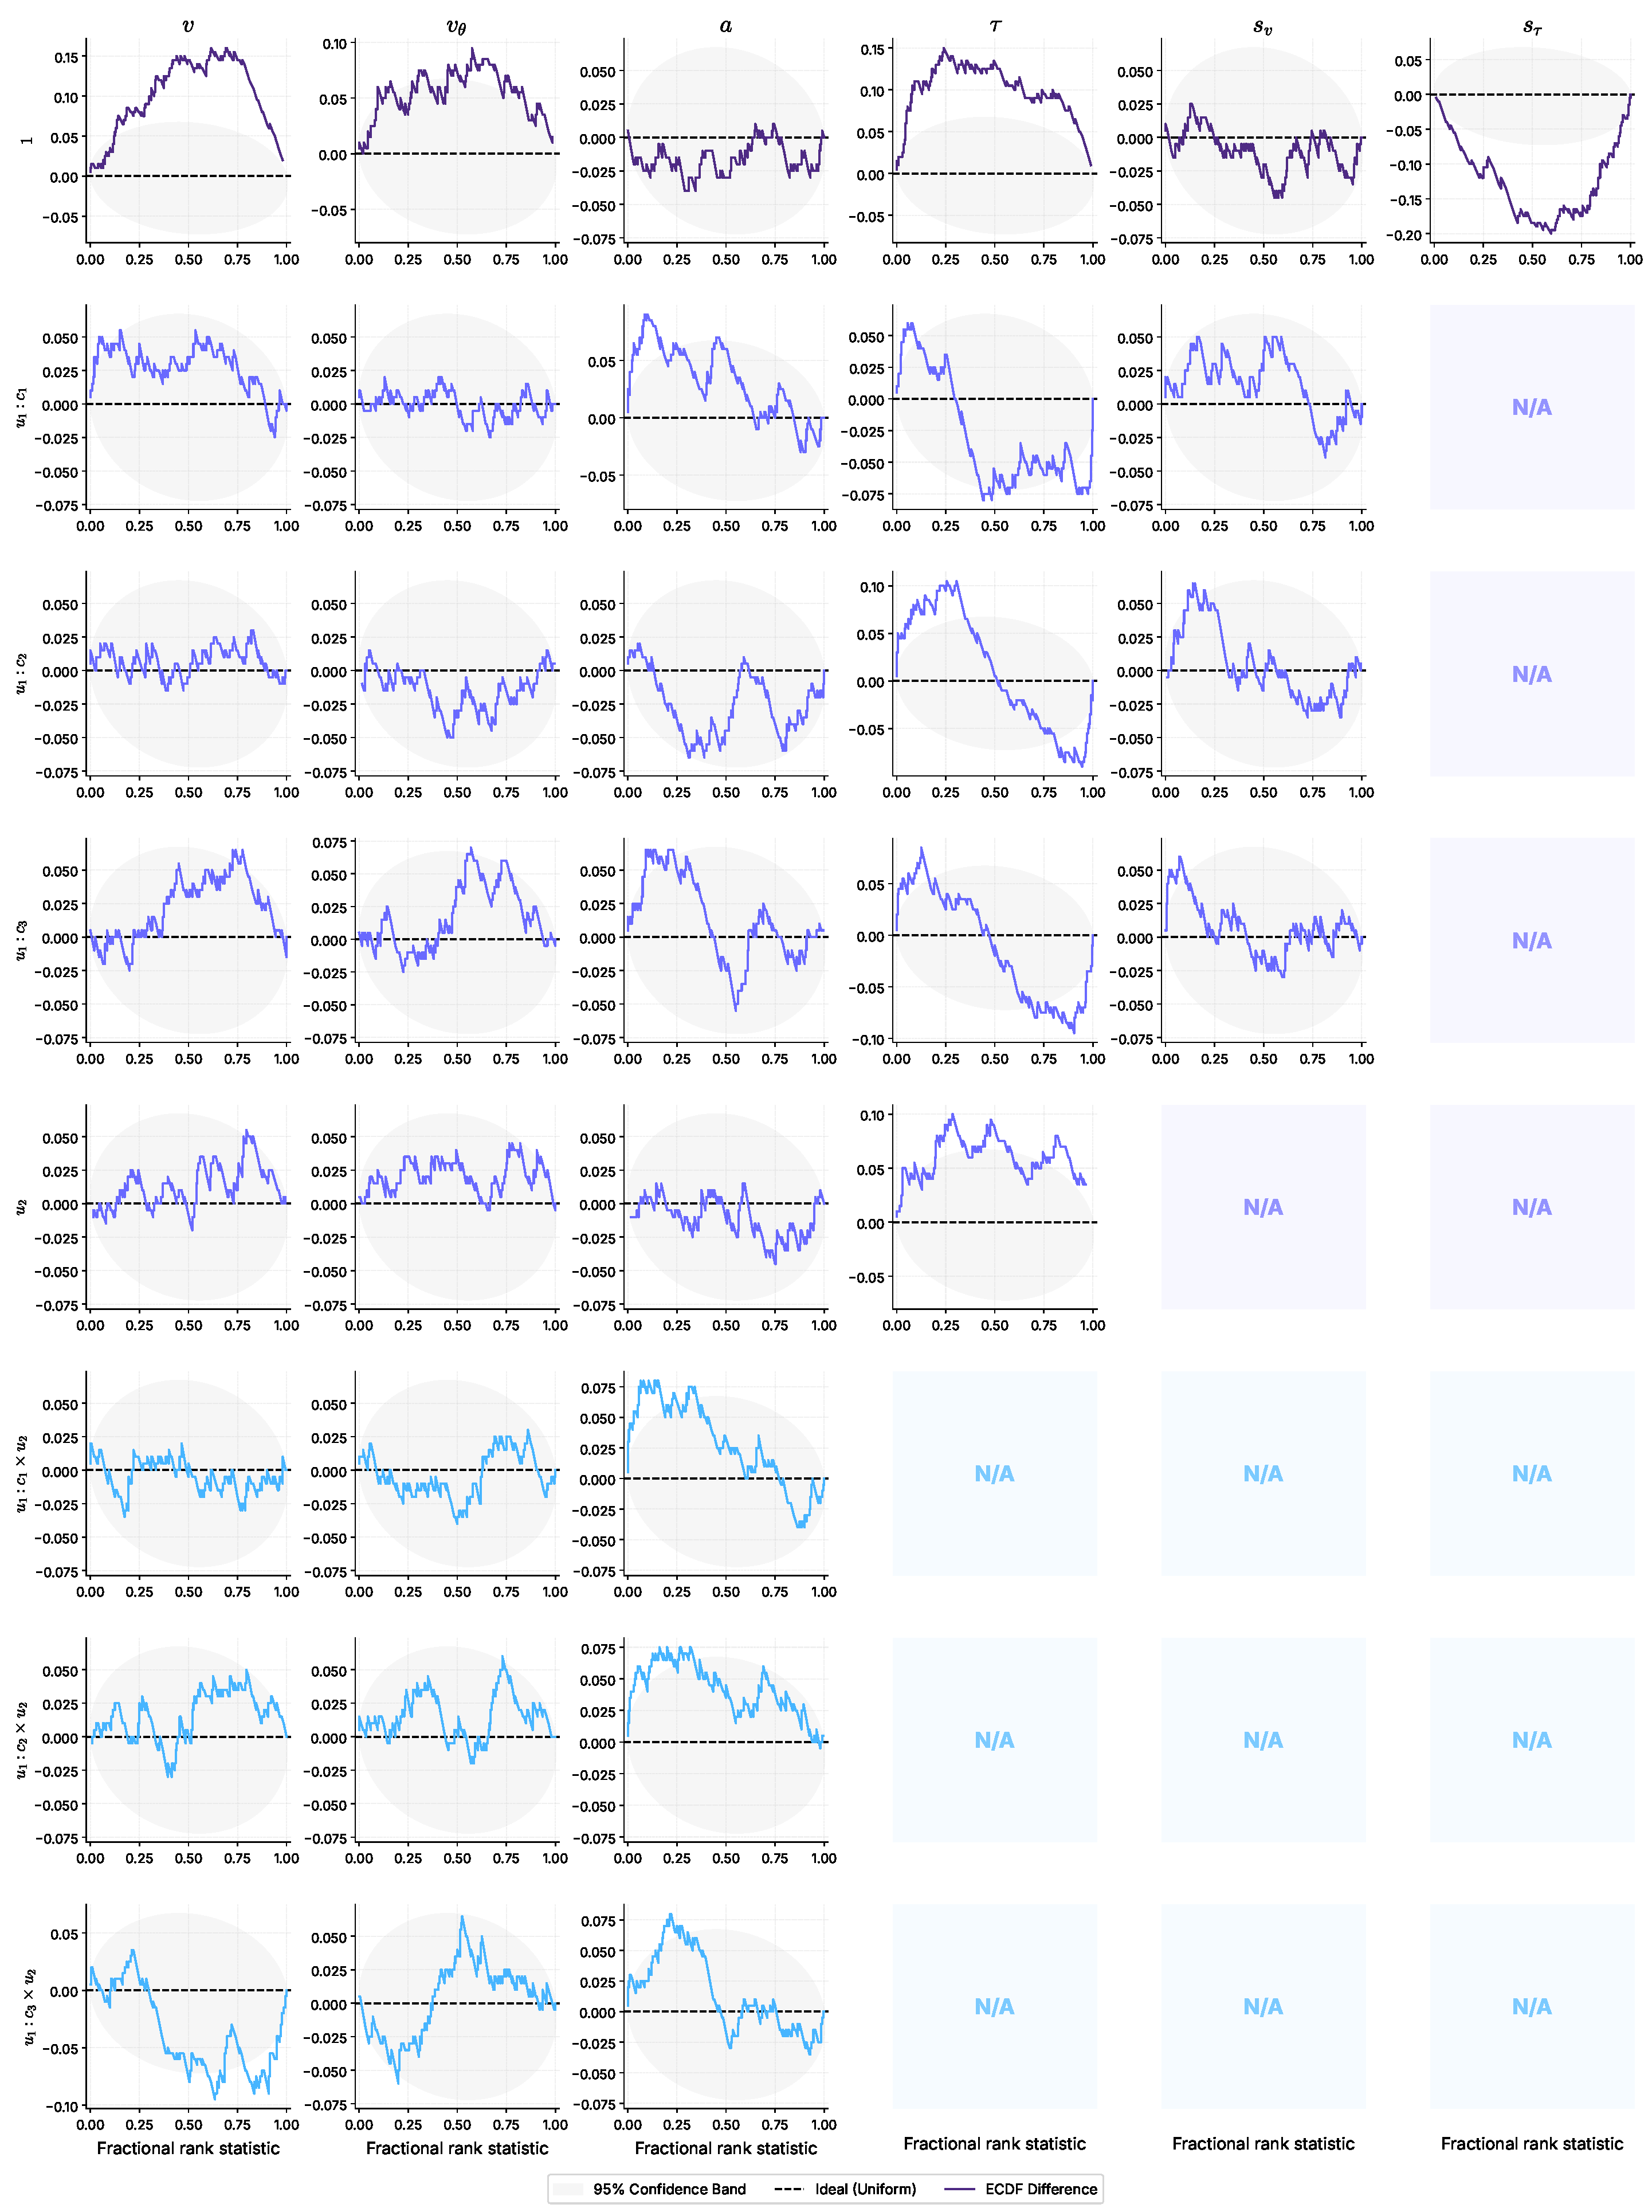
\includegraphics[width=\textwidth,height=0.82\textheight,keepaspectratio]{per_case/cdm/mixed_predictor/ecdf.pdf}
  \caption{\textbf{Simulation-based calibration, CDM, \emph{mixed-predictor} design (CogFormer).} $v$, $v_\theta$, $a$, $\tau$ and $s_v$ carry effects of $u_1$; $v$, $v_\theta$, $a$ and $\tau$ carry slopes on $u_2$; $v$, $v_\theta$ and $a$ carry the interaction (34 coefficients shown). Design as in Figure~\ref{fig:app1-ddm-mixed-predictor-recovery}; encoding as in panel (b) of Figure~\ref{fig:app1-ddm-intercept-only-cf}.}
  \label{fig:app1-cdm-mixed-predictor-ecdf}
\end{figure}

\begin{figure}[p]
  \centering
  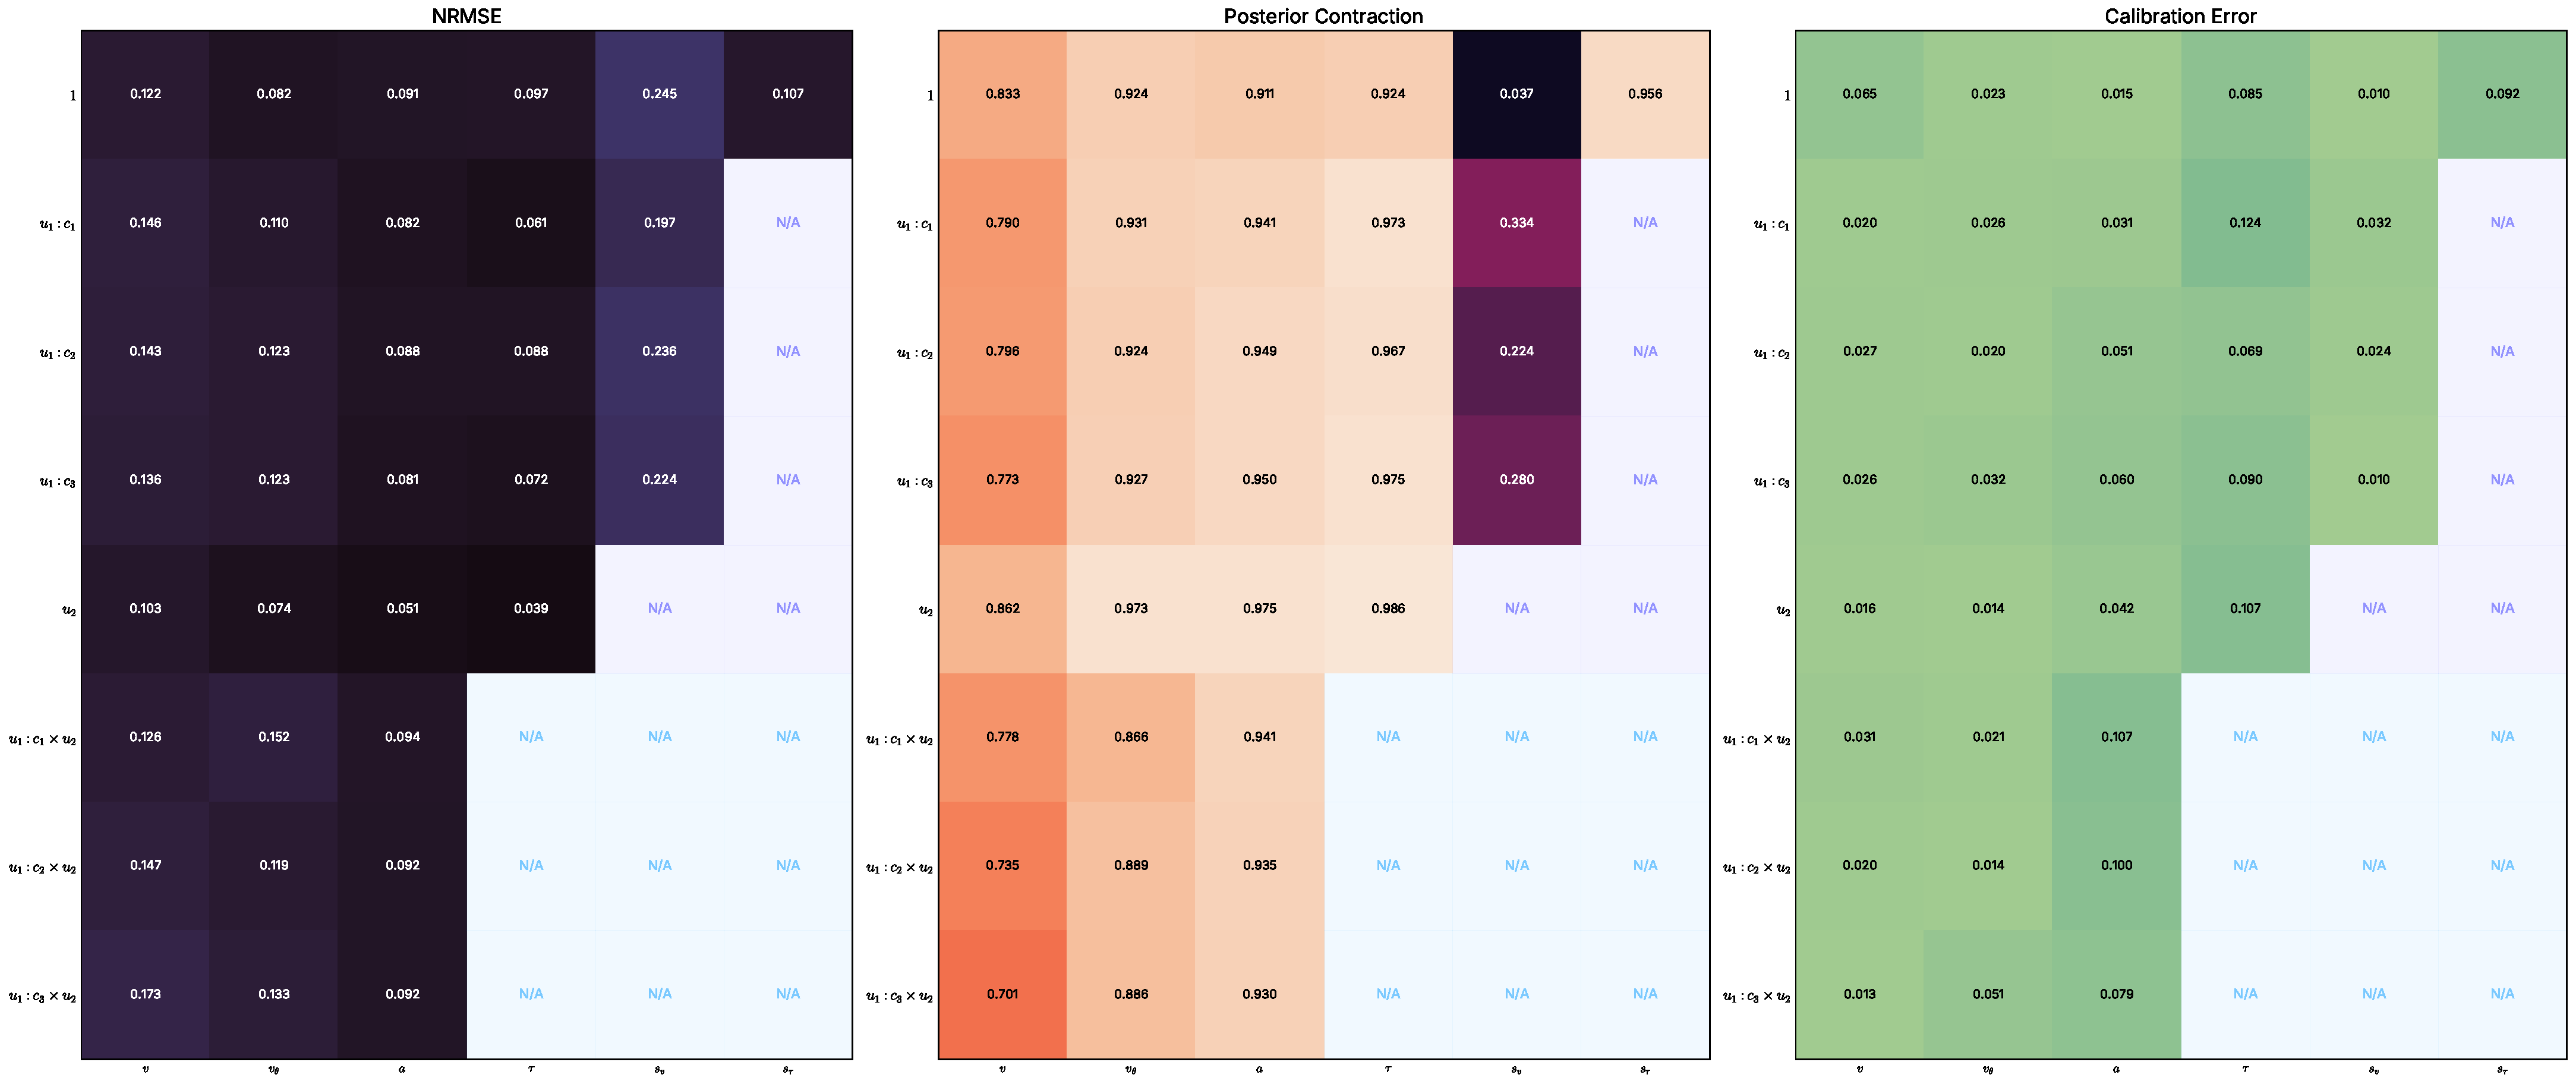
\includegraphics[width=\textwidth,height=0.82\textheight,keepaspectratio]{per_case/cdm/mixed_predictor/metrics.pdf}
  \caption{\textbf{Summary metrics, CDM, \emph{mixed-predictor} design (CogFormer).} $v$, $v_\theta$, $a$, $\tau$ and $s_v$ carry effects of $u_1$; $v$, $v_\theta$, $a$ and $\tau$ carry slopes on $u_2$; $v$, $v_\theta$ and $a$ carry the interaction (34 coefficients shown). Design as in Figure~\ref{fig:app1-ddm-mixed-predictor-recovery}; encoding as in panel (c) of Figure~\ref{fig:app1-ddm-intercept-only-cf}.}
  \label{fig:app1-cdm-mixed-predictor-metrics}
\end{figure}

% ── benchmark ensembles ──

\begin{figure}[p]
  \centering
  \begin{subfigure}{\textwidth}\centering
    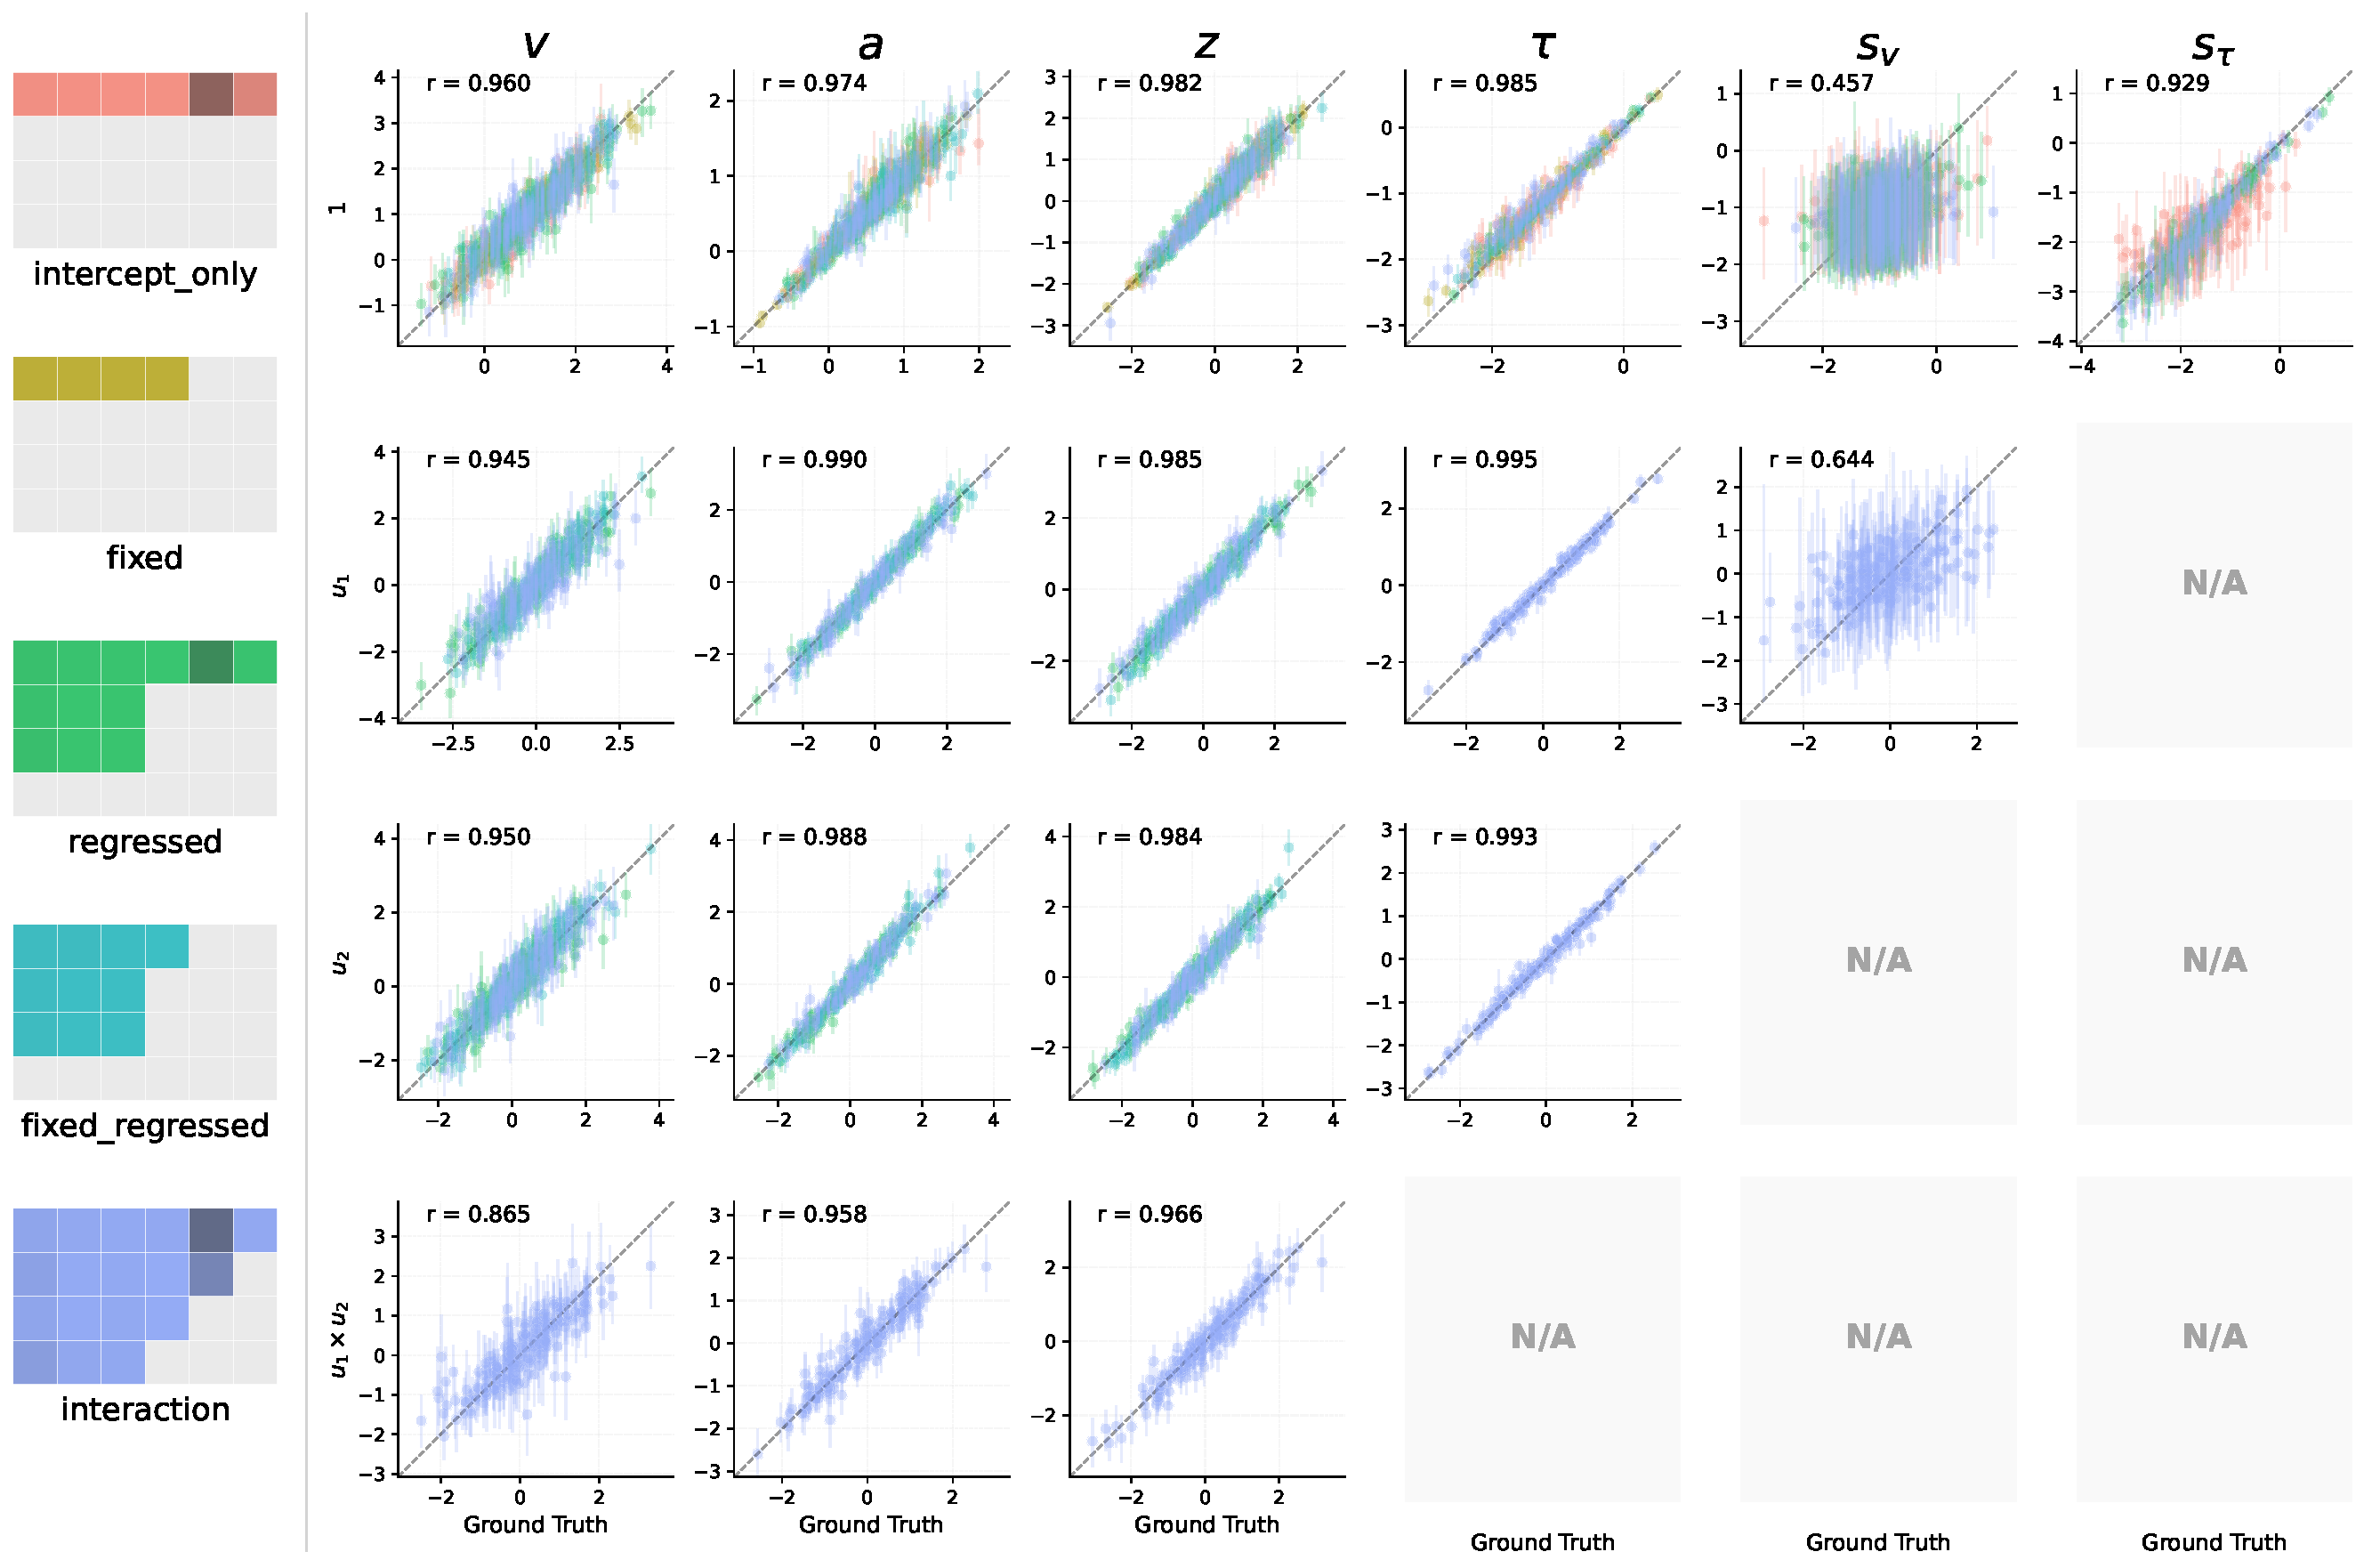
\includegraphics[width=\textwidth,height=0.3\textheight,keepaspectratio]{benchmark_ensemble/bench5/ddm/recovery.pdf}
    \caption{Recovery}
  \end{subfigure}\\[1ex]
  \begin{subfigure}{\textwidth}\centering
    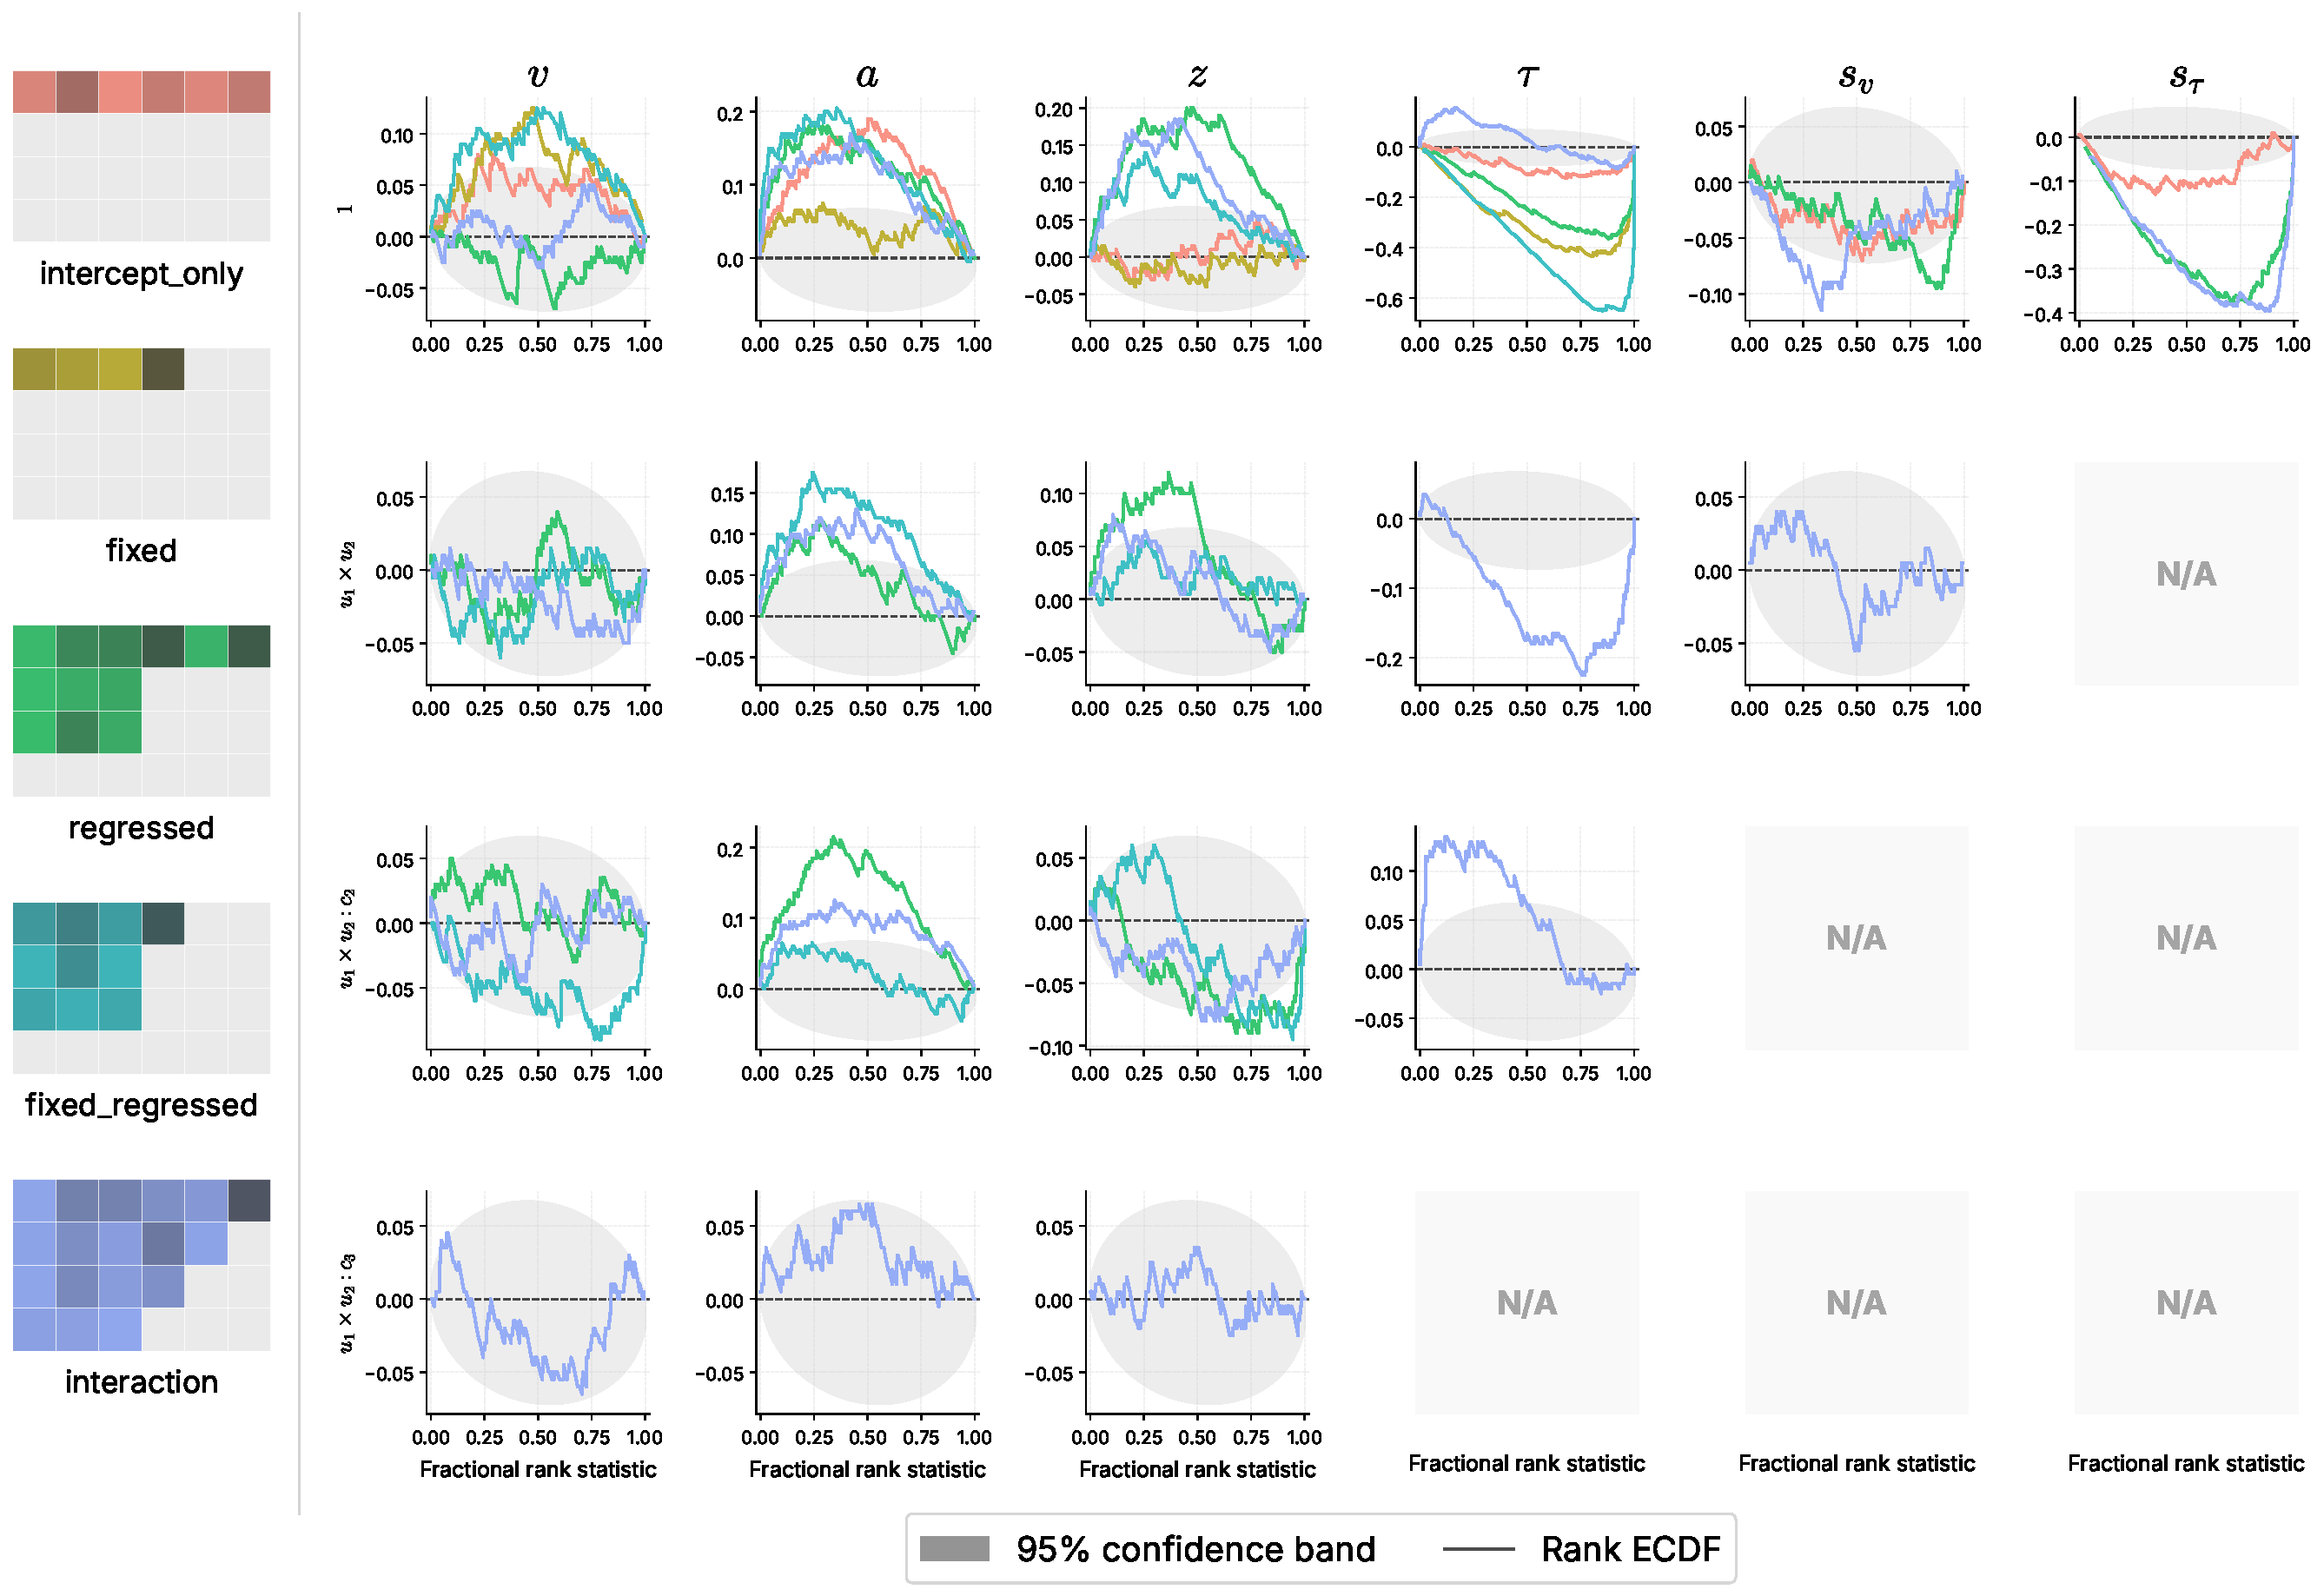
\includegraphics[width=\textwidth,height=0.3\textheight,keepaspectratio]{benchmark_ensemble/bench5/ddm/ecdf.pdf}
    \caption{Calibration (ECDF)}
  \end{subfigure}\\[1ex]
  \begin{subfigure}{\textwidth}\centering
    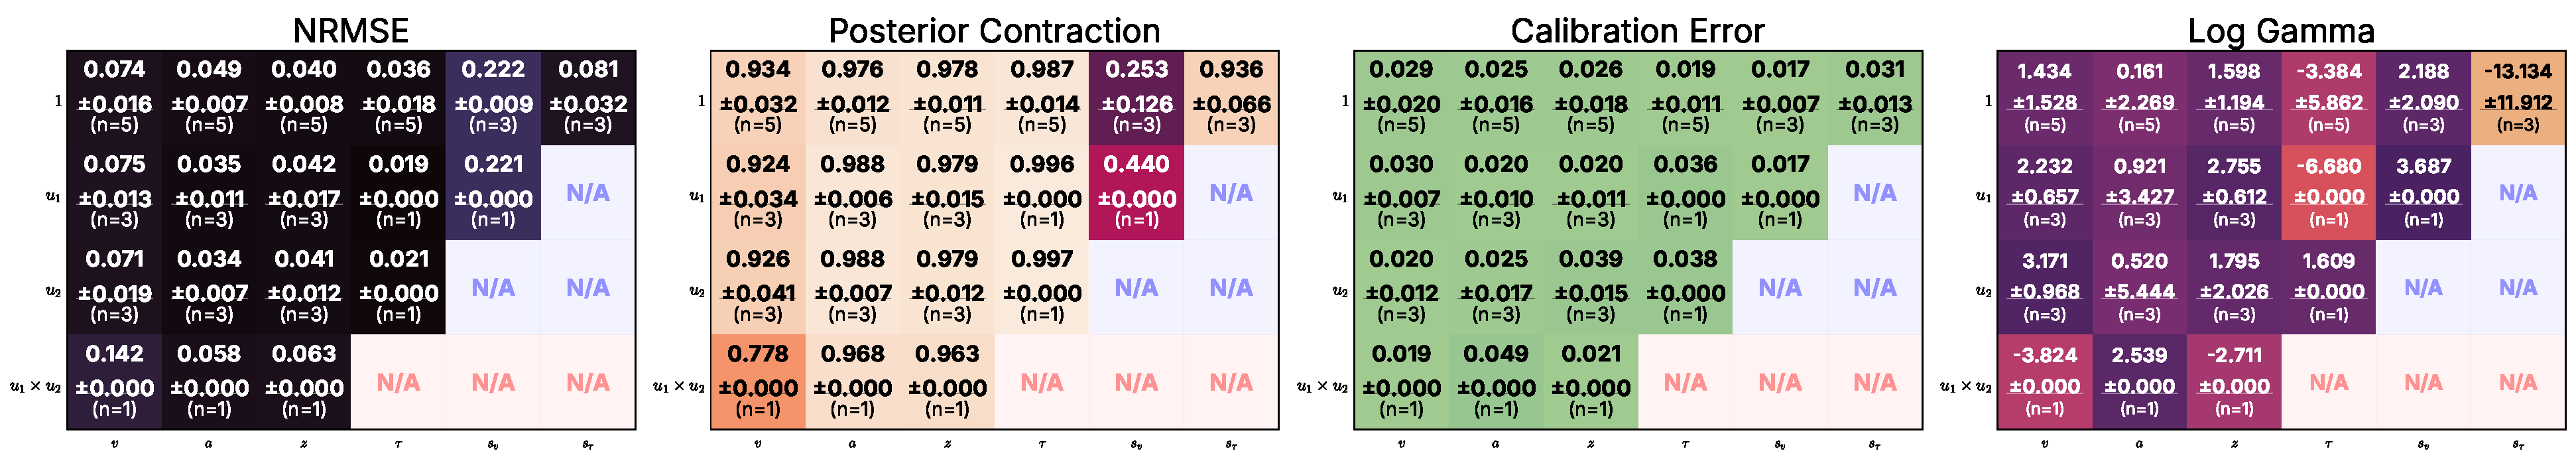
\includegraphics[width=\textwidth]{benchmark_ensemble/bench5/ddm/metrics.pdf}
    \caption{Metrics}
  \end{subfigure}
  \caption{\textbf{Benchmark ensemble, DDM: the five benchmark designs overlaid (CogFormer).} (a) Parameter recovery, (b) calibration and (c) summary metrics of the intercept-only, fixed, regressed, fixed + regressed and interaction designs on one coefficient grid; each design contributes its 200 bench5 test datasets (500 trials, 200 posterior draws each), and a cell pools every design that contains that coefficient. Rows and columns as in Figure~\ref{fig:app1-ddm-intercept-only-cf}; $\pi$ is not shown. (a) Posterior means against ground truth, one colour per design, with central 90\% credible intervals; $r$ is the mean over designs of the per-design Pearson correlation. The strip on the left draws each design's coefficient pattern in its colour, with cell opacity proportional to that design's $|r|$ (floored at 0.2), so poorly recovered coefficients appear faint. (b) Rank-ECDF difference curves, one per design, against the common pointwise 95\% band for 200 uniform ranks; reading as in panel (b) of Figure~\ref{fig:app1-ddm-intercept-only-cf}. (c) Each metric of panel (c) of Figure~\ref{fig:app1-ddm-intercept-only-cf} computed per design, then shown as the mean $\pm$ standard deviation over the $n$ designs that contain the coefficient, coloured by the mean. The fourth heatmap, log $\gamma$, is the log ratio of the ECDF-based uniformity statistic $\gamma$ of the calibration ranks to the 5\% quantile of its null distribution under uniform ranks: values below zero reject calibration at the 5\% level, values above zero do not; its colour scale spans the observed range. Figures~\ref{fig:app1-rdm-bench5}--\ref{fig:app1-cdm-bench5} show the other two families in the same way, followed by the six-design ensembles.}
  \label{fig:app1-ddm-bench5}
\end{figure}

\begin{figure}[p]
  \centering
  \begin{subfigure}{\textwidth}\centering
    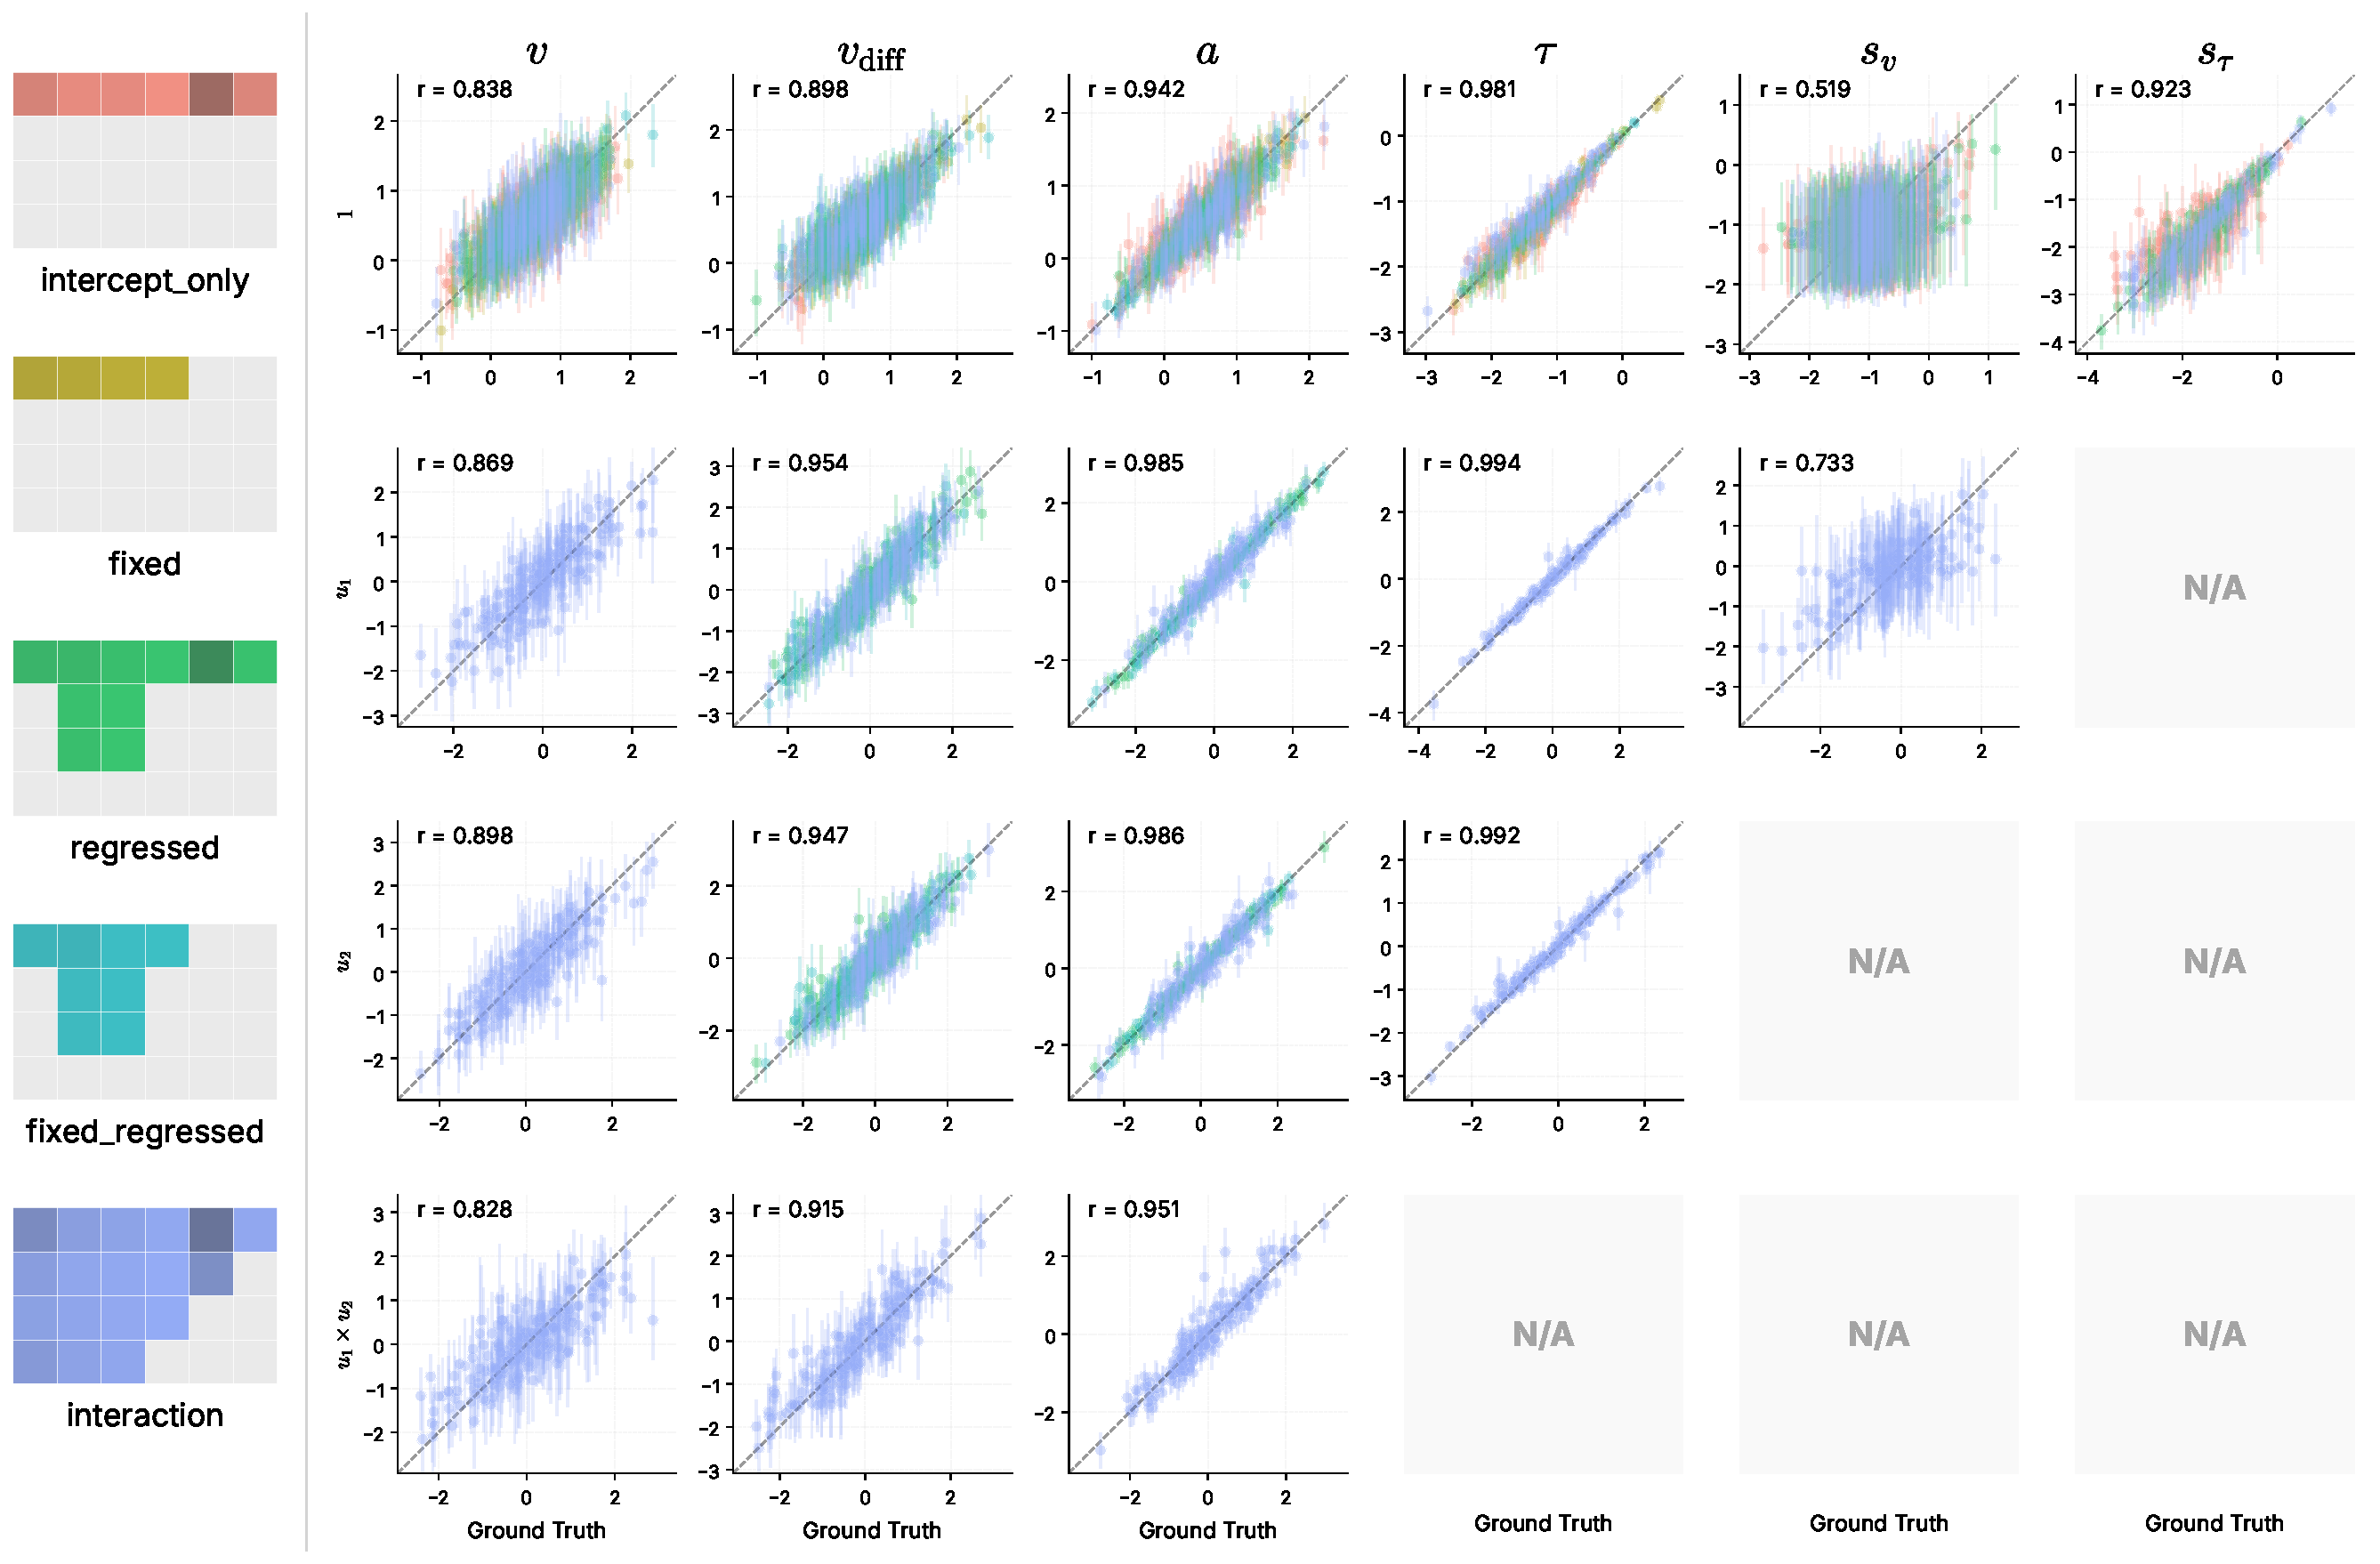
\includegraphics[width=\textwidth,height=0.3\textheight,keepaspectratio]{benchmark_ensemble/bench5/rdm/recovery.pdf}
    \caption{Recovery}
  \end{subfigure}\\[1ex]
  \begin{subfigure}{\textwidth}\centering
    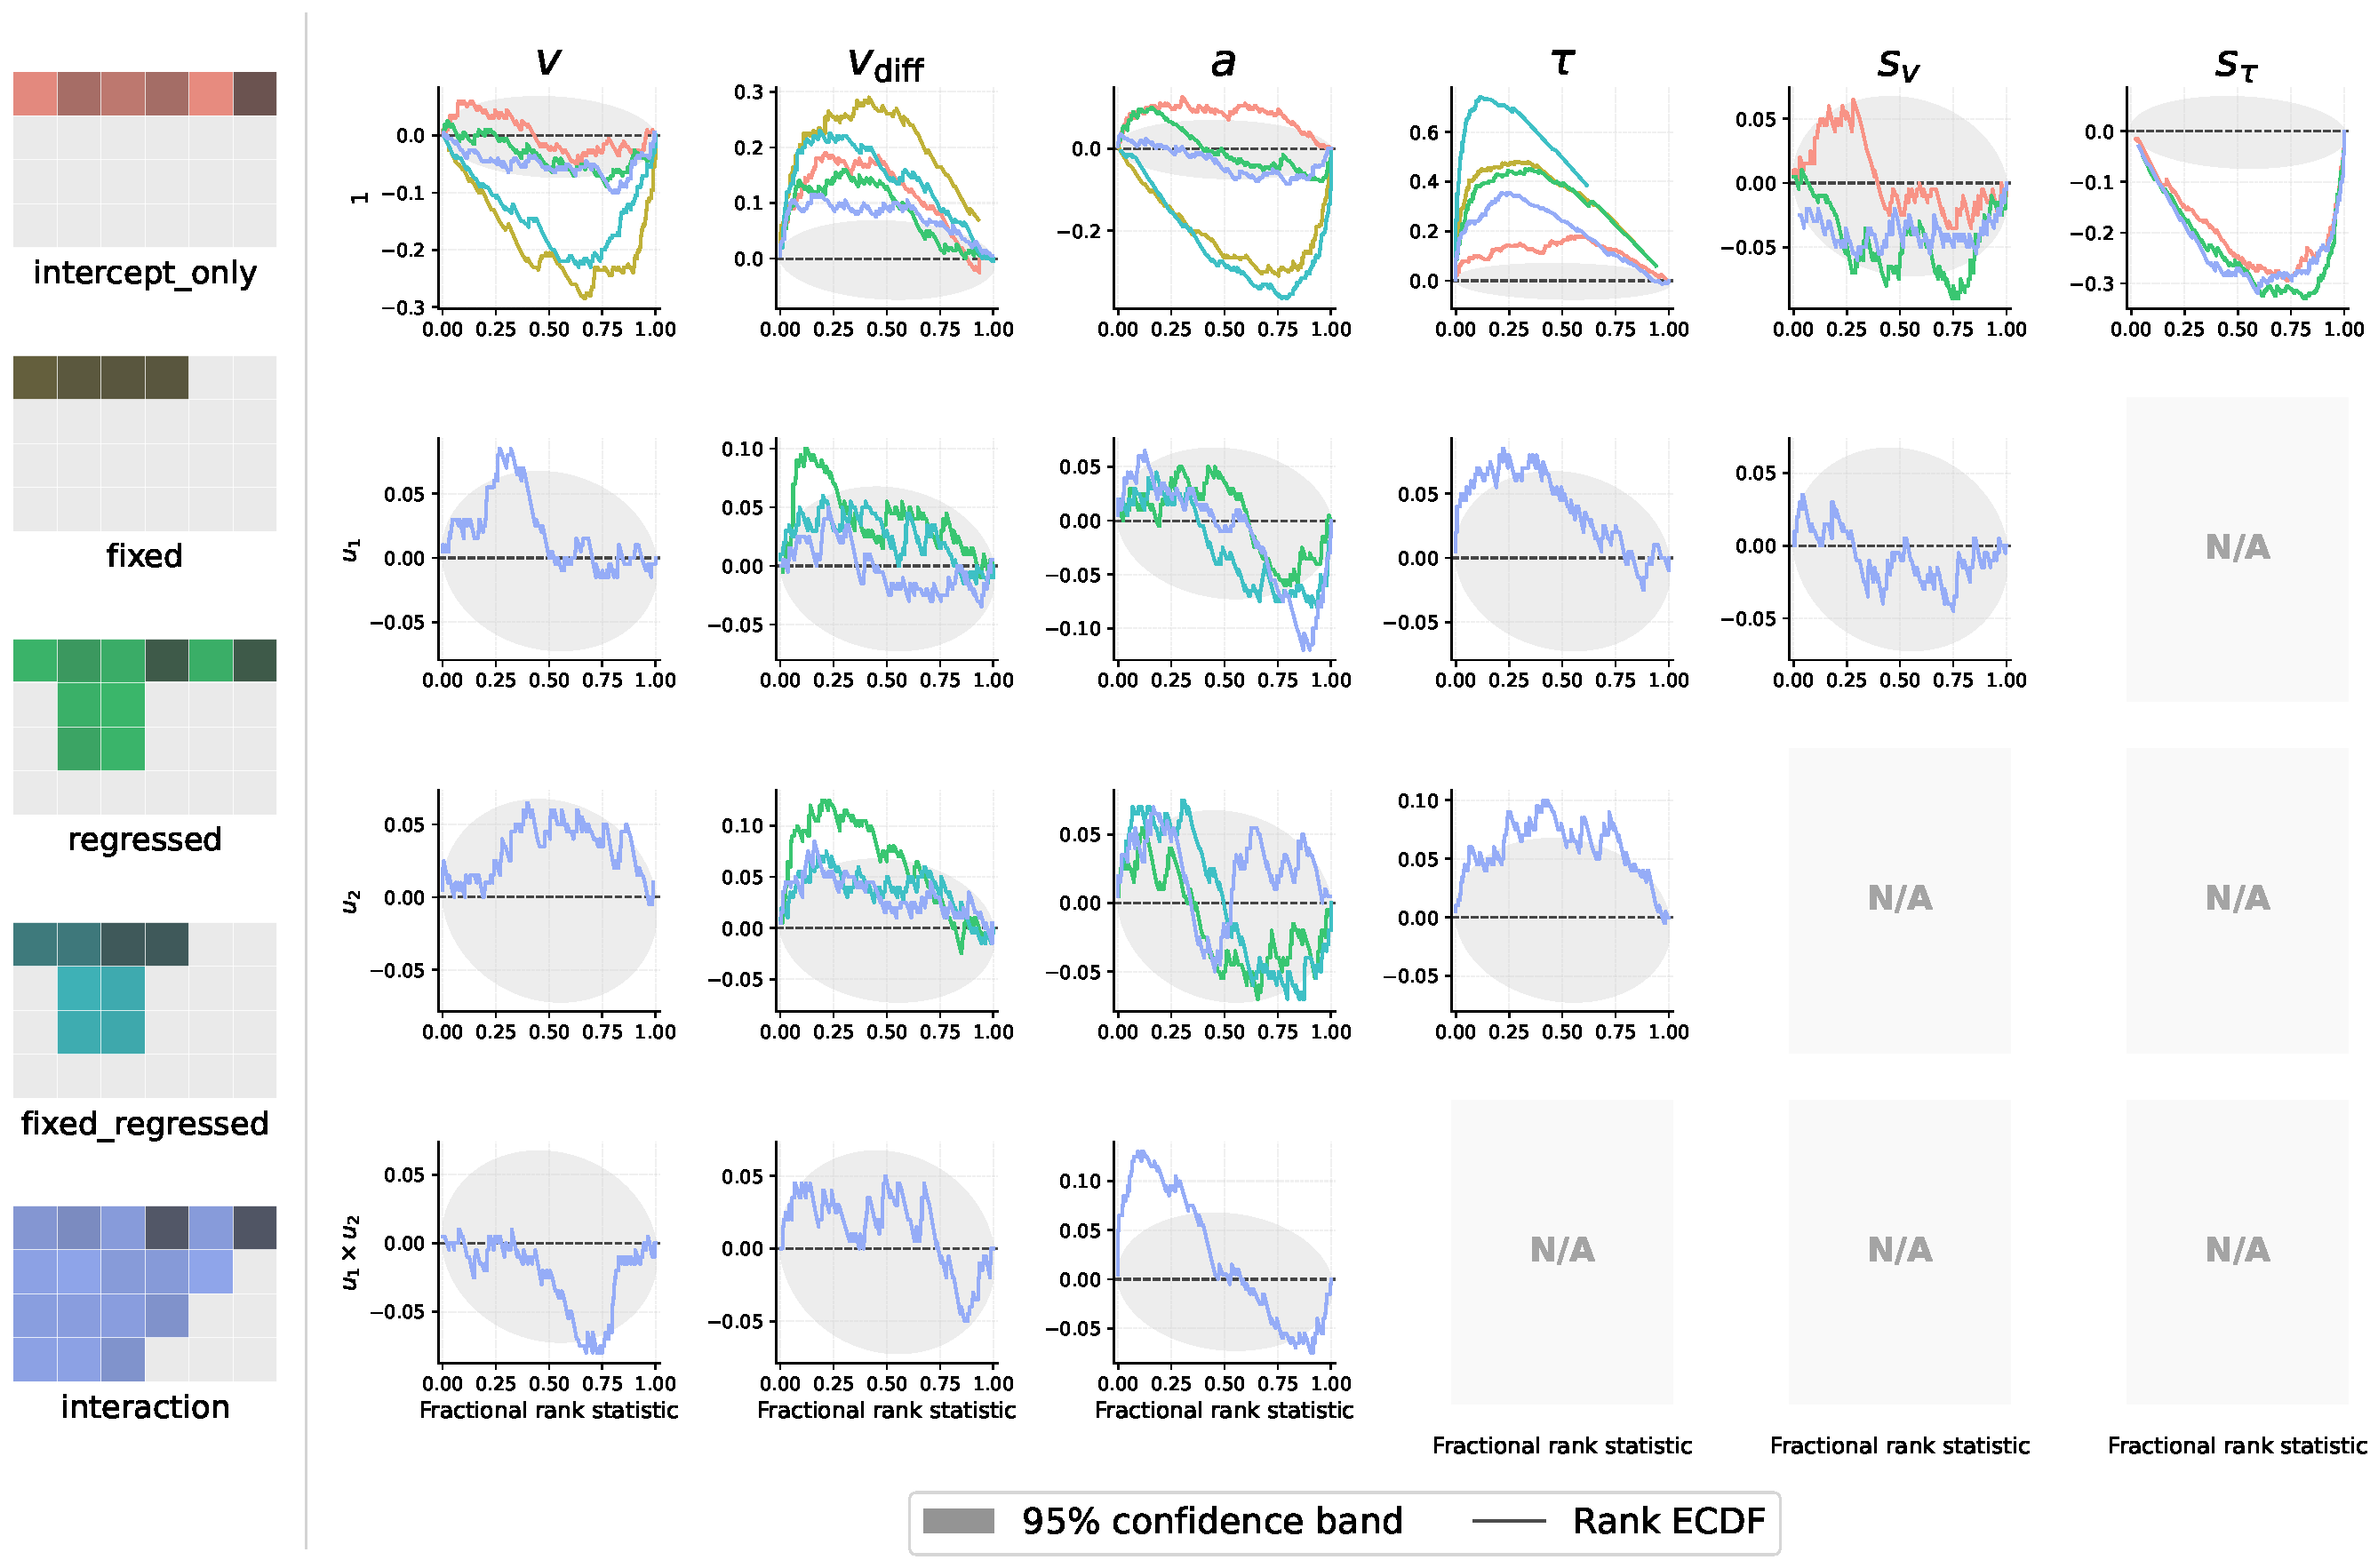
\includegraphics[width=\textwidth,height=0.3\textheight,keepaspectratio]{benchmark_ensemble/bench5/rdm/ecdf.pdf}
    \caption{Calibration (ECDF)}
  \end{subfigure}\\[1ex]
  \begin{subfigure}{\textwidth}\centering
    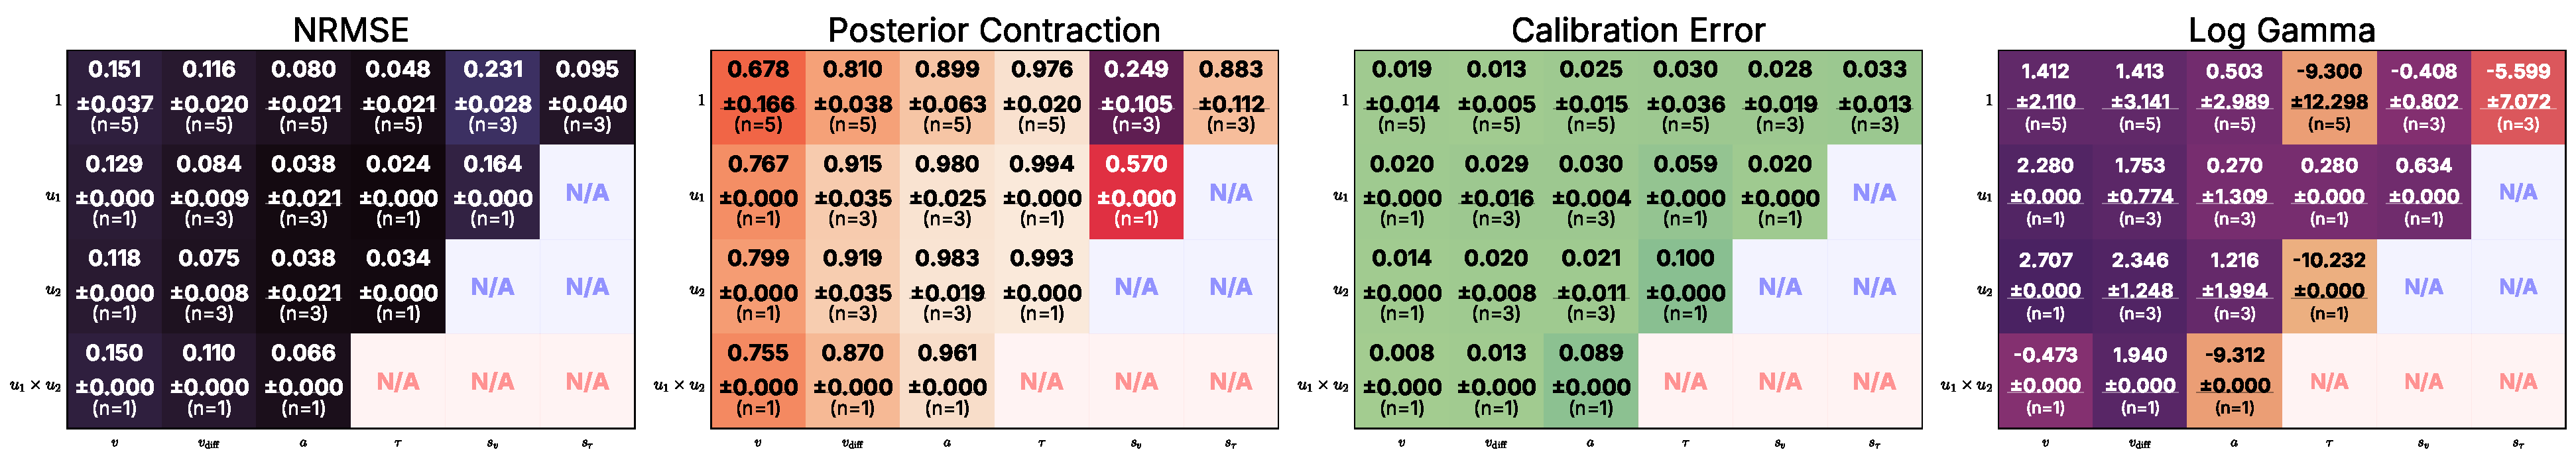
\includegraphics[width=\textwidth]{benchmark_ensemble/bench5/rdm/metrics.pdf}
    \caption{Metrics}
  \end{subfigure}
  \caption{\textbf{Benchmark ensemble, RDM: the five benchmark designs overlaid (CogFormer).} (a) Recovery, (b) calibration, (c) metrics. Layout and encoding as in Figure~\ref{fig:app1-ddm-bench5}.}
  \label{fig:app1-rdm-bench5}
\end{figure}

\begin{figure}[p]
  \centering
  \begin{subfigure}{\textwidth}\centering
    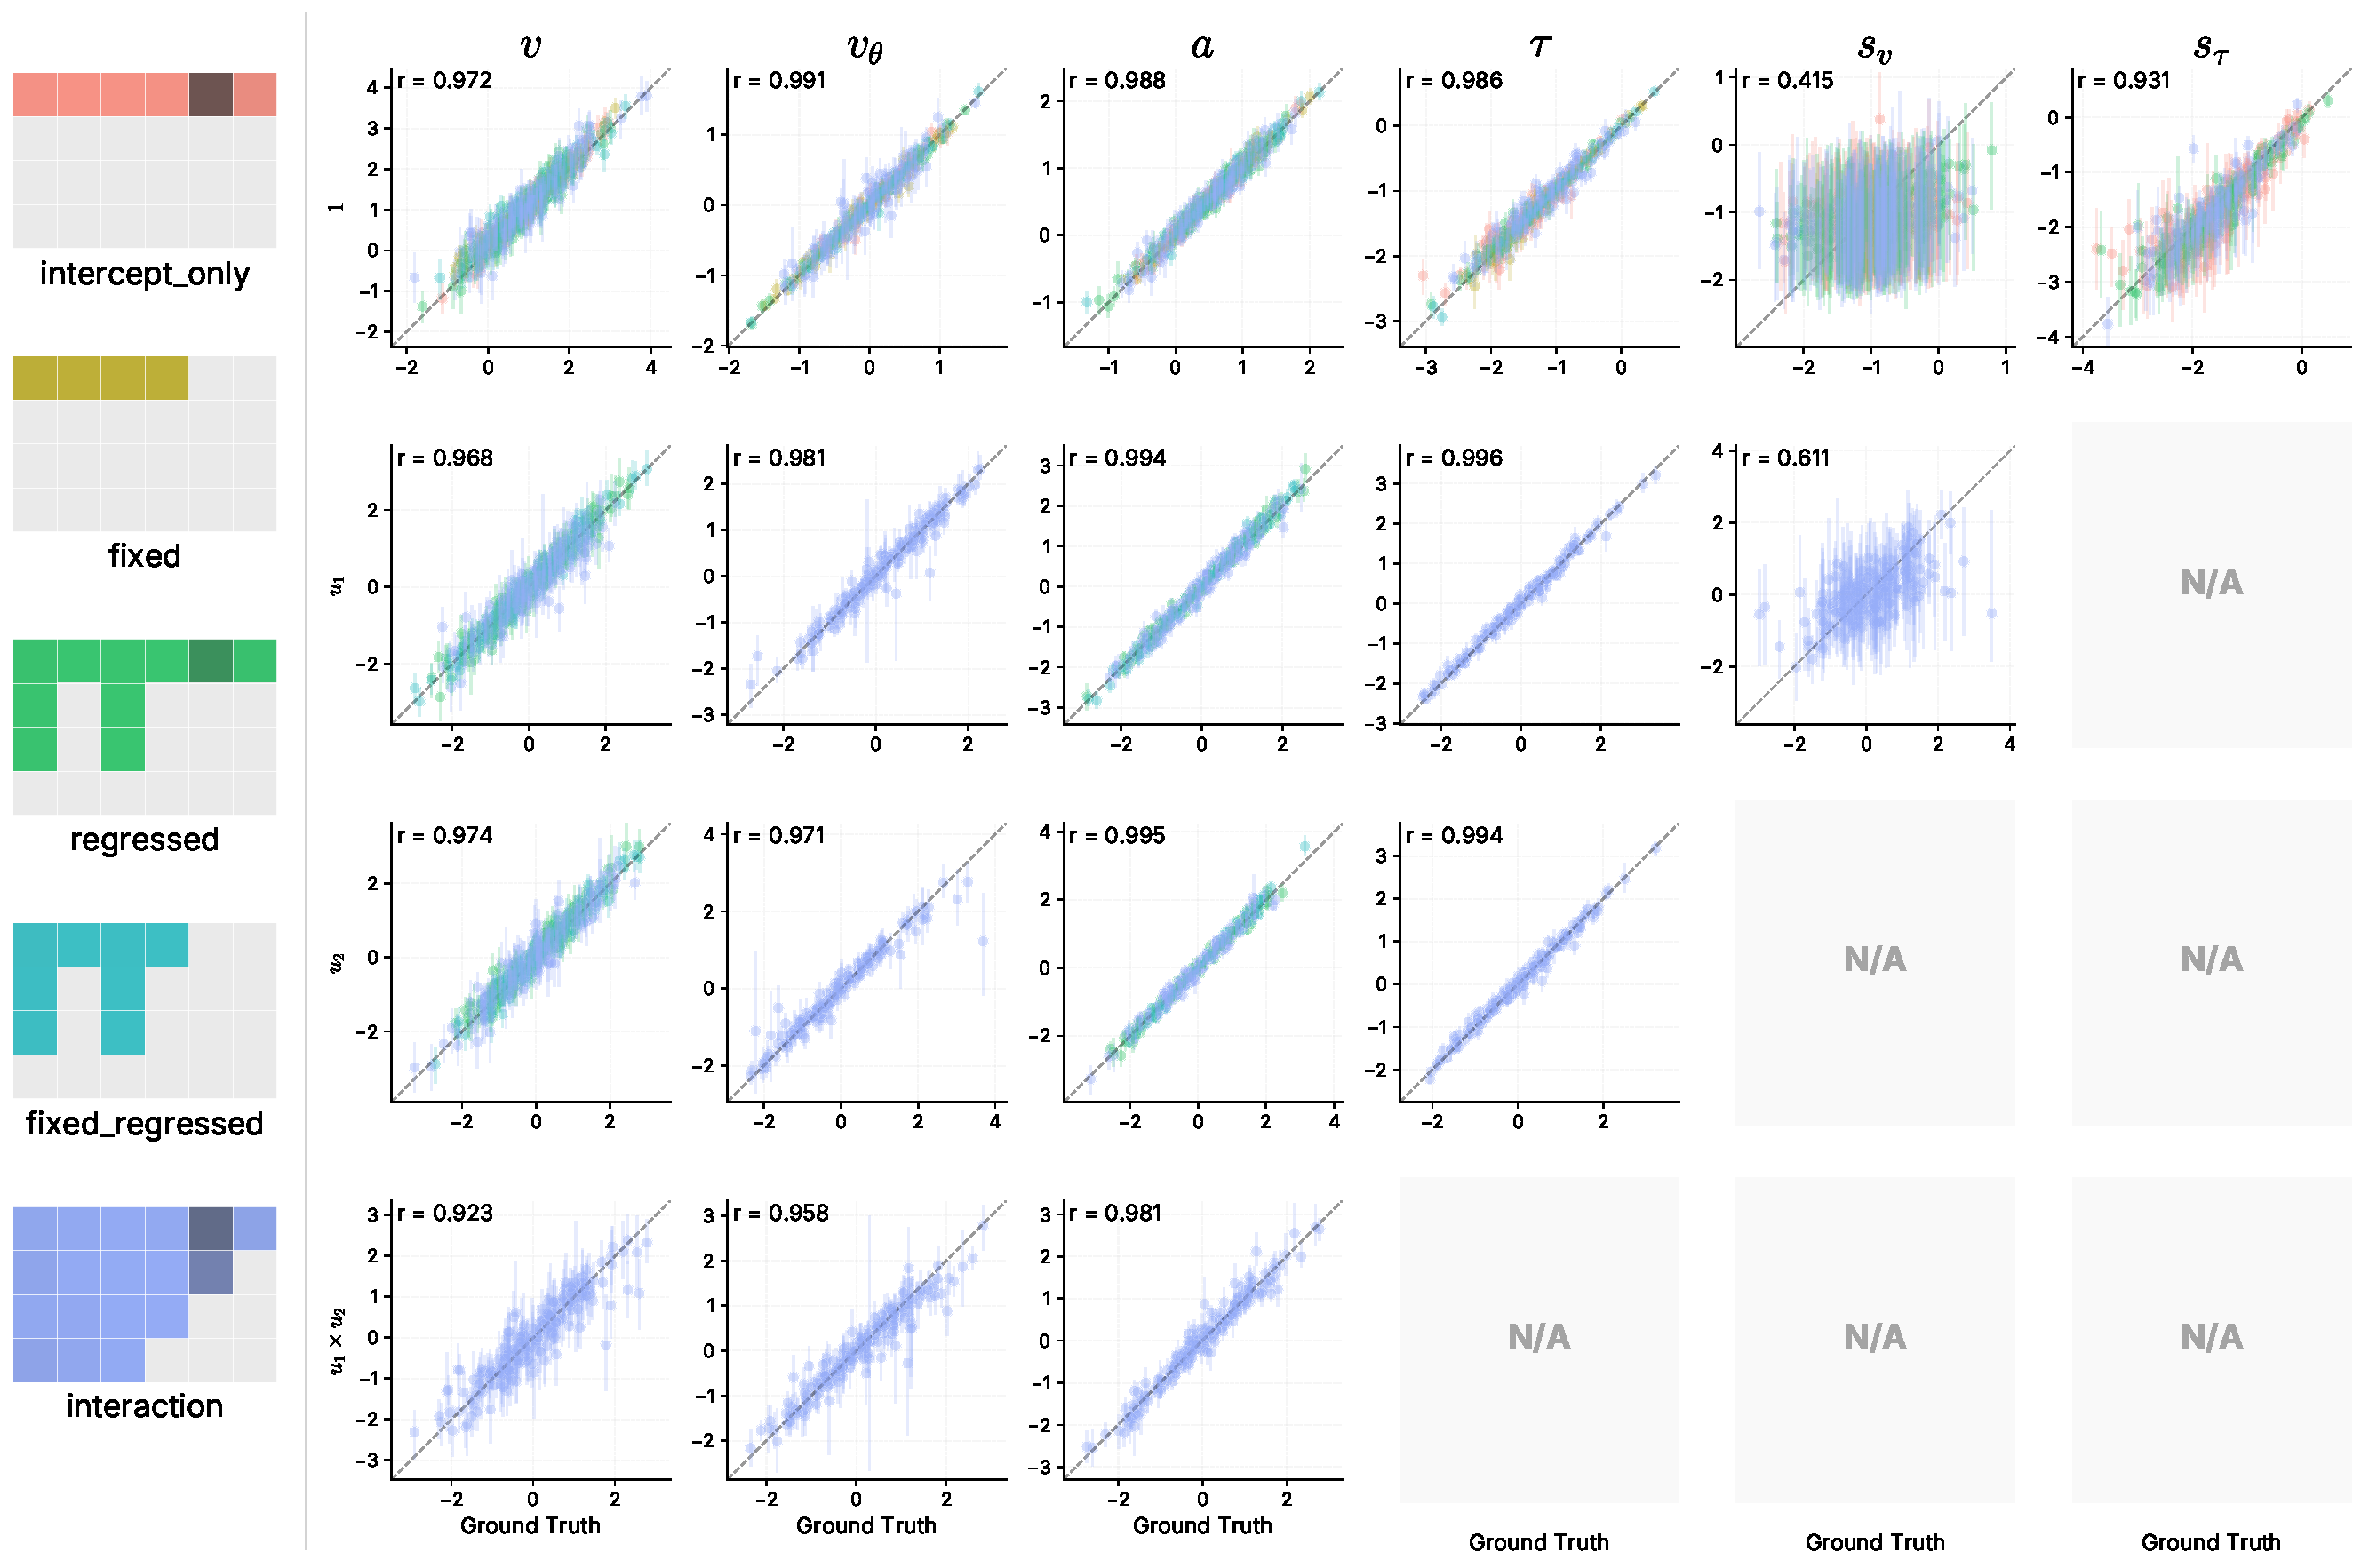
\includegraphics[width=\textwidth,height=0.3\textheight,keepaspectratio]{benchmark_ensemble/bench5/cdm/recovery.pdf}
    \caption{Recovery}
  \end{subfigure}\\[1ex]
  \begin{subfigure}{\textwidth}\centering
    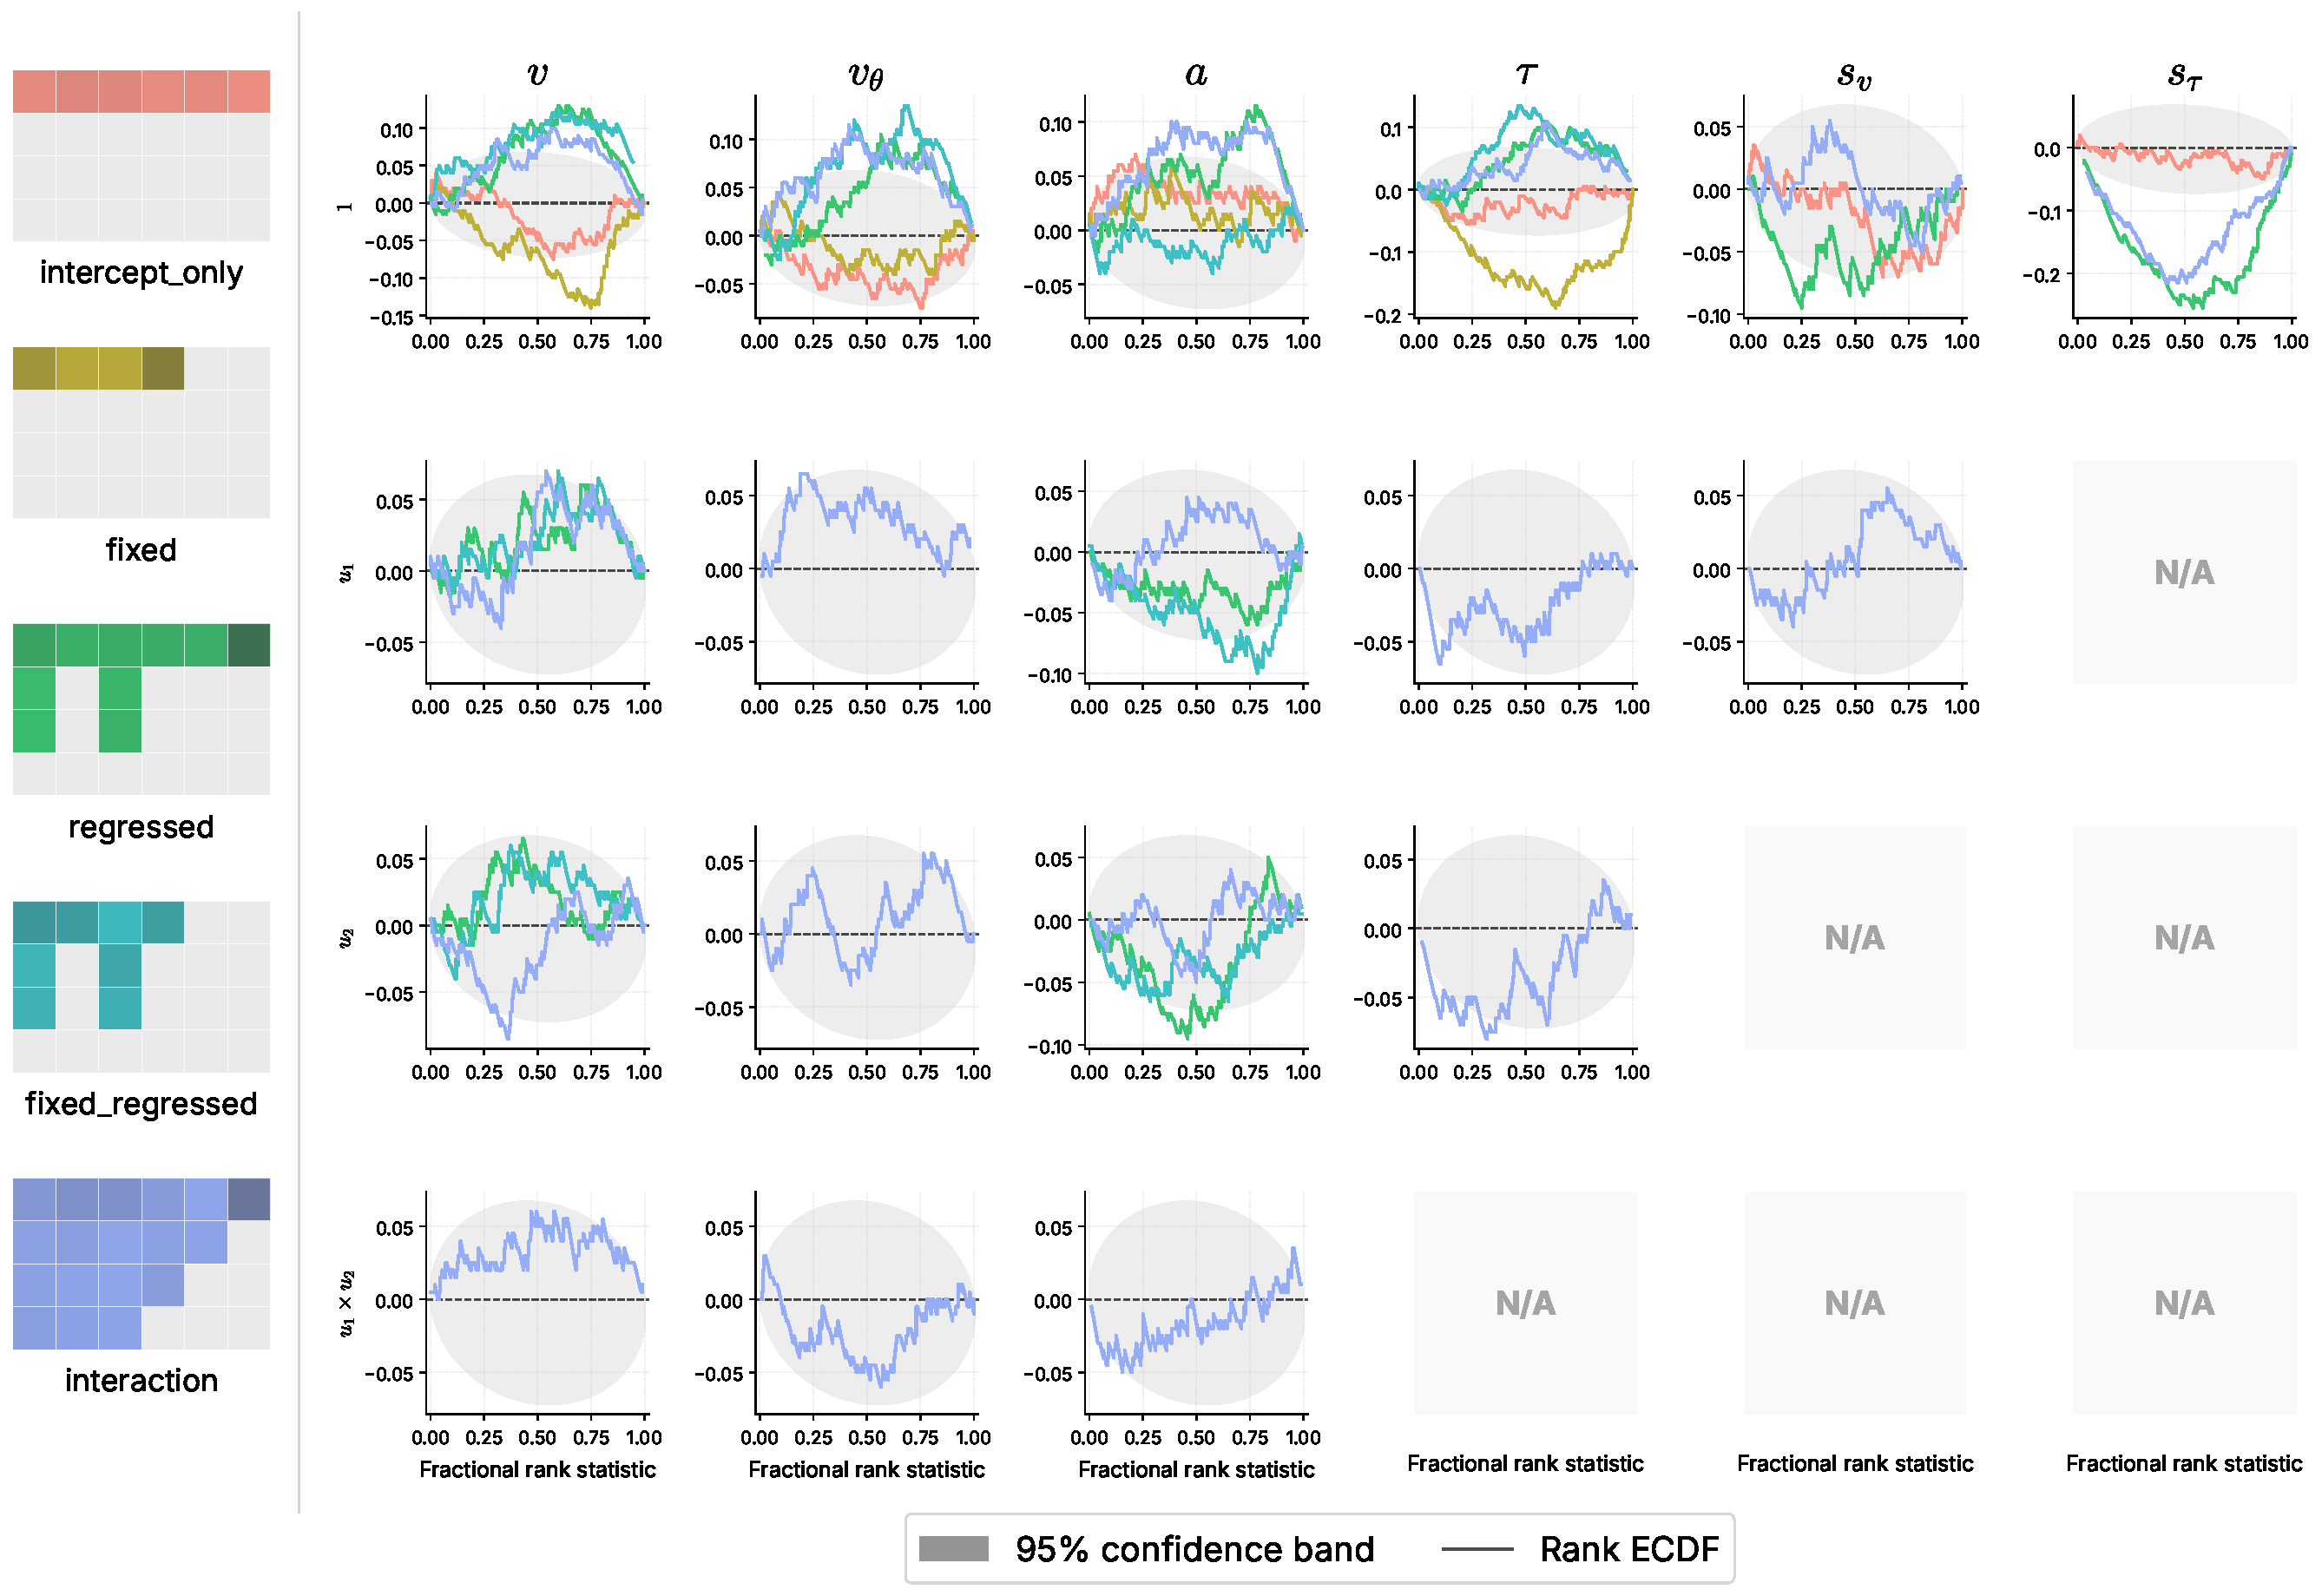
\includegraphics[width=\textwidth,height=0.3\textheight,keepaspectratio]{benchmark_ensemble/bench5/cdm/ecdf.pdf}
    \caption{Calibration (ECDF)}
  \end{subfigure}\\[1ex]
  \begin{subfigure}{\textwidth}\centering
    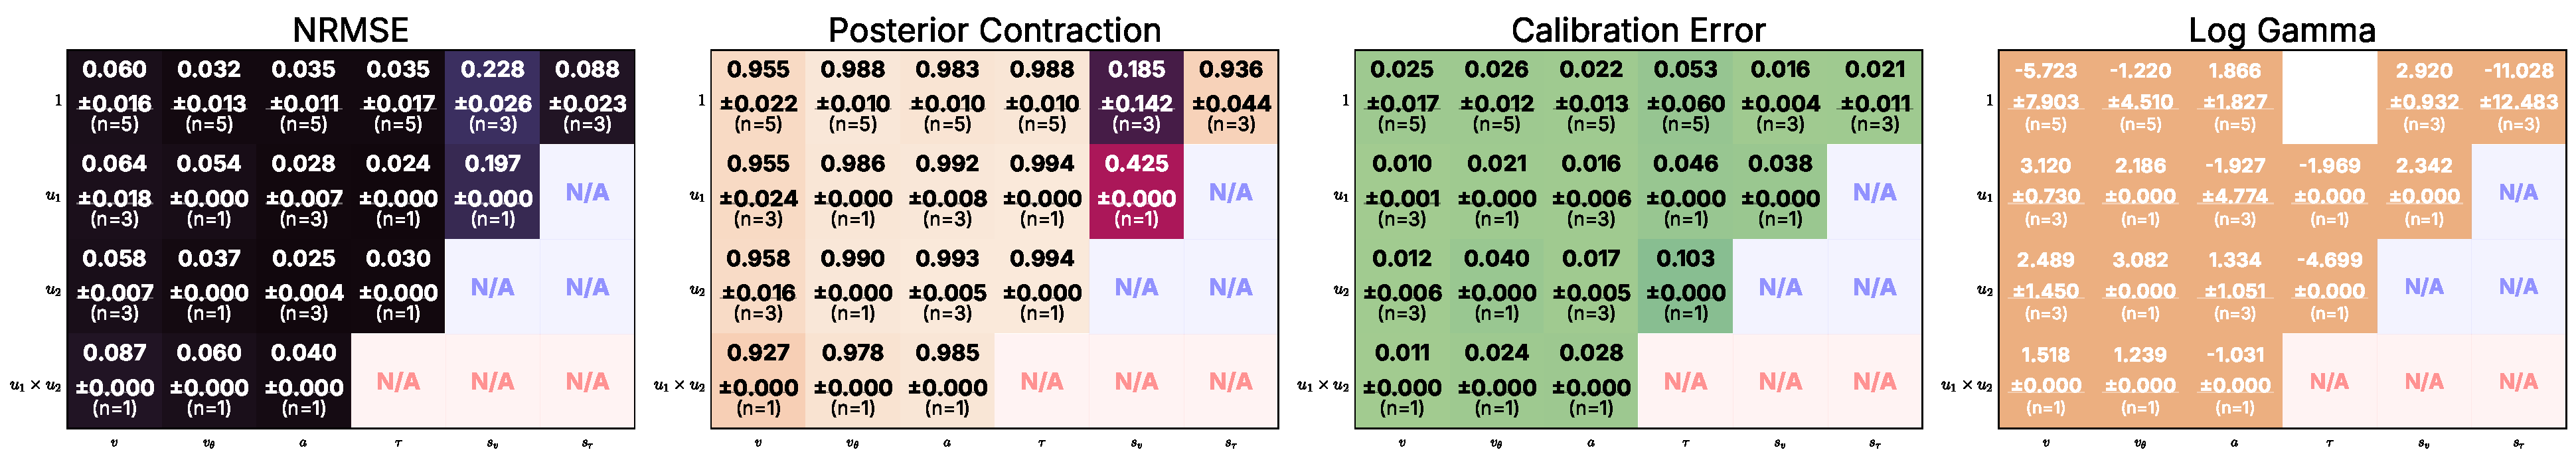
\includegraphics[width=\textwidth]{benchmark_ensemble/bench5/cdm/metrics.pdf}
    \caption{Metrics}
  \end{subfigure}
  \caption{\textbf{Benchmark ensemble, CDM: the five benchmark designs overlaid (CogFormer).} (a) Recovery, (b) calibration, (c) metrics. Layout and encoding as in Figure~\ref{fig:app1-ddm-bench5}.}
  \label{fig:app1-cdm-bench5}
\end{figure}

\begin{figure}[p]
  \centering
  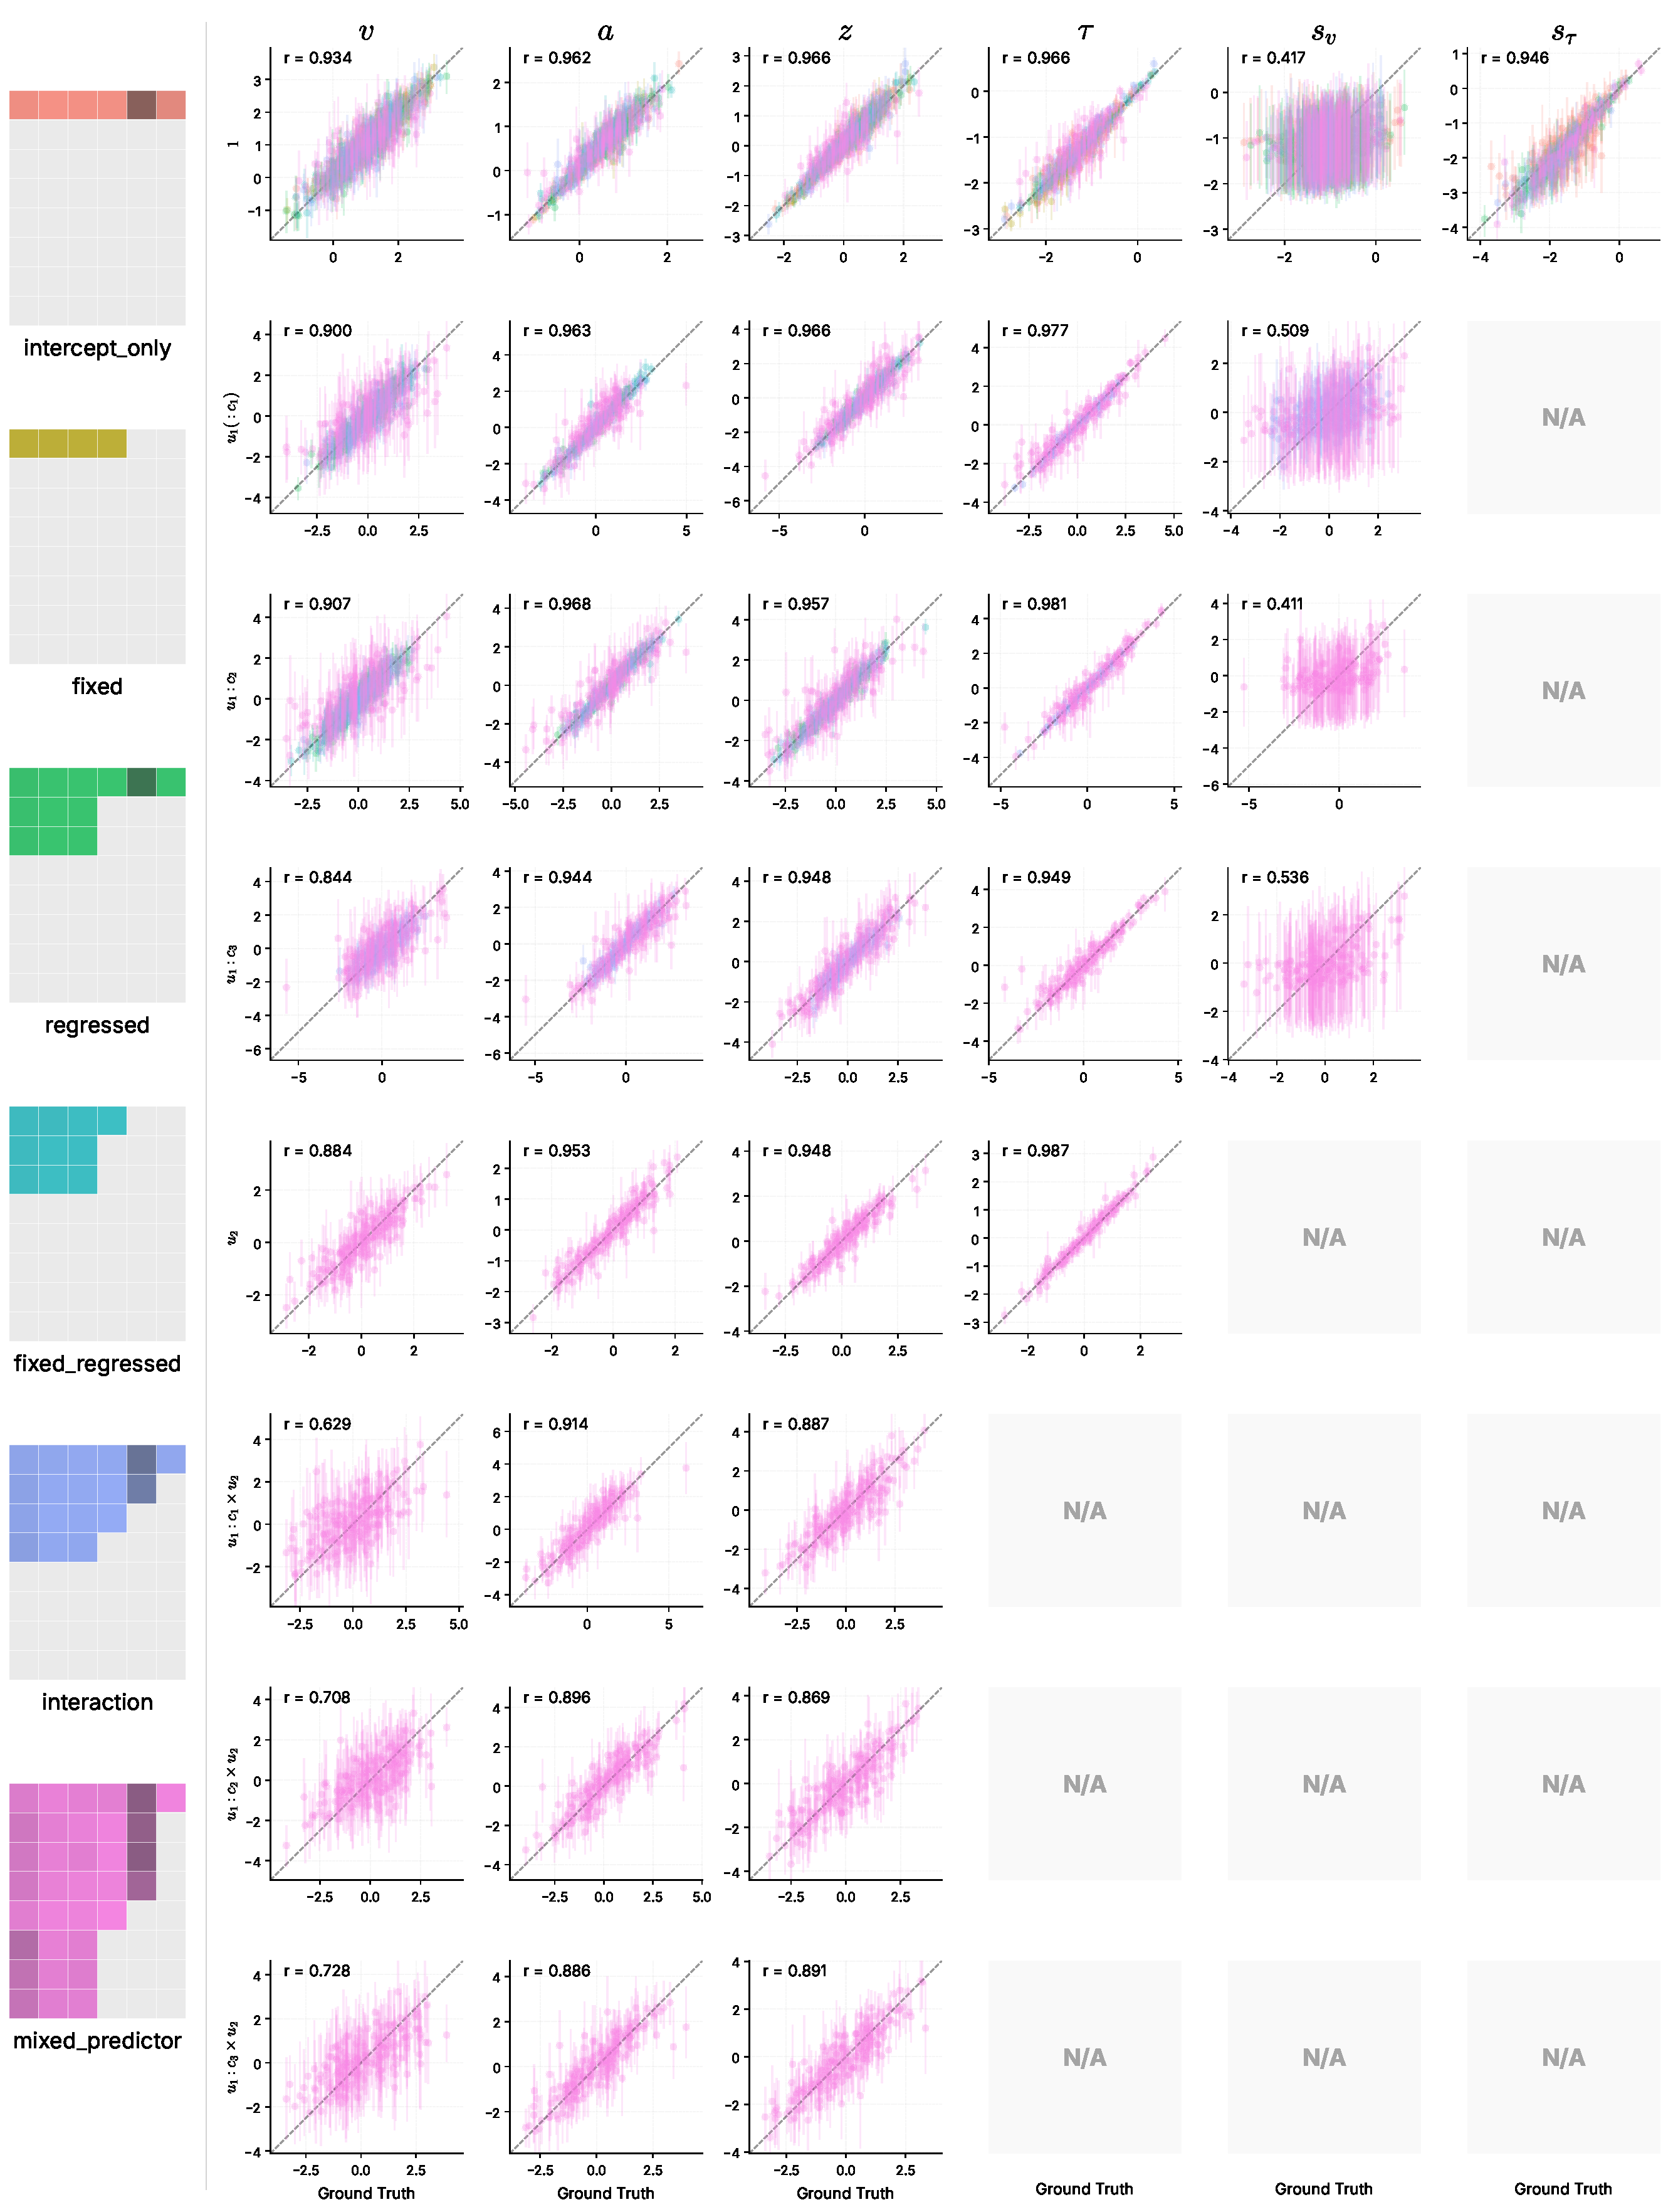
\includegraphics[width=\textwidth,height=0.82\textheight,keepaspectratio]{benchmark_ensemble/bench6/ddm/recovery.pdf}
  \caption{\textbf{Parameter recovery, six-design benchmark ensemble, DDM (CogFormer).} The five benchmark designs of Figure~\ref{fig:app1-ddm-bench5} plus the mixed-predictor design (Figure~\ref{fig:app1-ddm-mixed-predictor-recovery}), overlaid on one grid in the mixed-predictor design's layout. The first contrast of the categorical $u_1$ shares a row with the continuous designs' $u_1$ slope, labelled $u_1(:c_1)$ (a slope or the first contrast, depending on the design), and likewise $u_1(:c_1) \times u_2$ for the interaction; the $u_2$ row pools every design with a $u_2$ slope, and the further contrast rows ($u_1{:}c_2$, $u_1{:}c_3$ and their interactions with $u_2$) come from the mixed-predictor design alone. Encoding as in panel (a) of Figure~\ref{fig:app1-ddm-bench5}. Shown separately because the grid is long; Figures~\ref{fig:app1-ddm-bench6-ecdf}--\ref{fig:app1-cdm-bench6-metrics} show the remaining diagnostics and families.}
  \label{fig:app1-ddm-bench6-recovery}
\end{figure}

\begin{figure}[p]
  \centering
  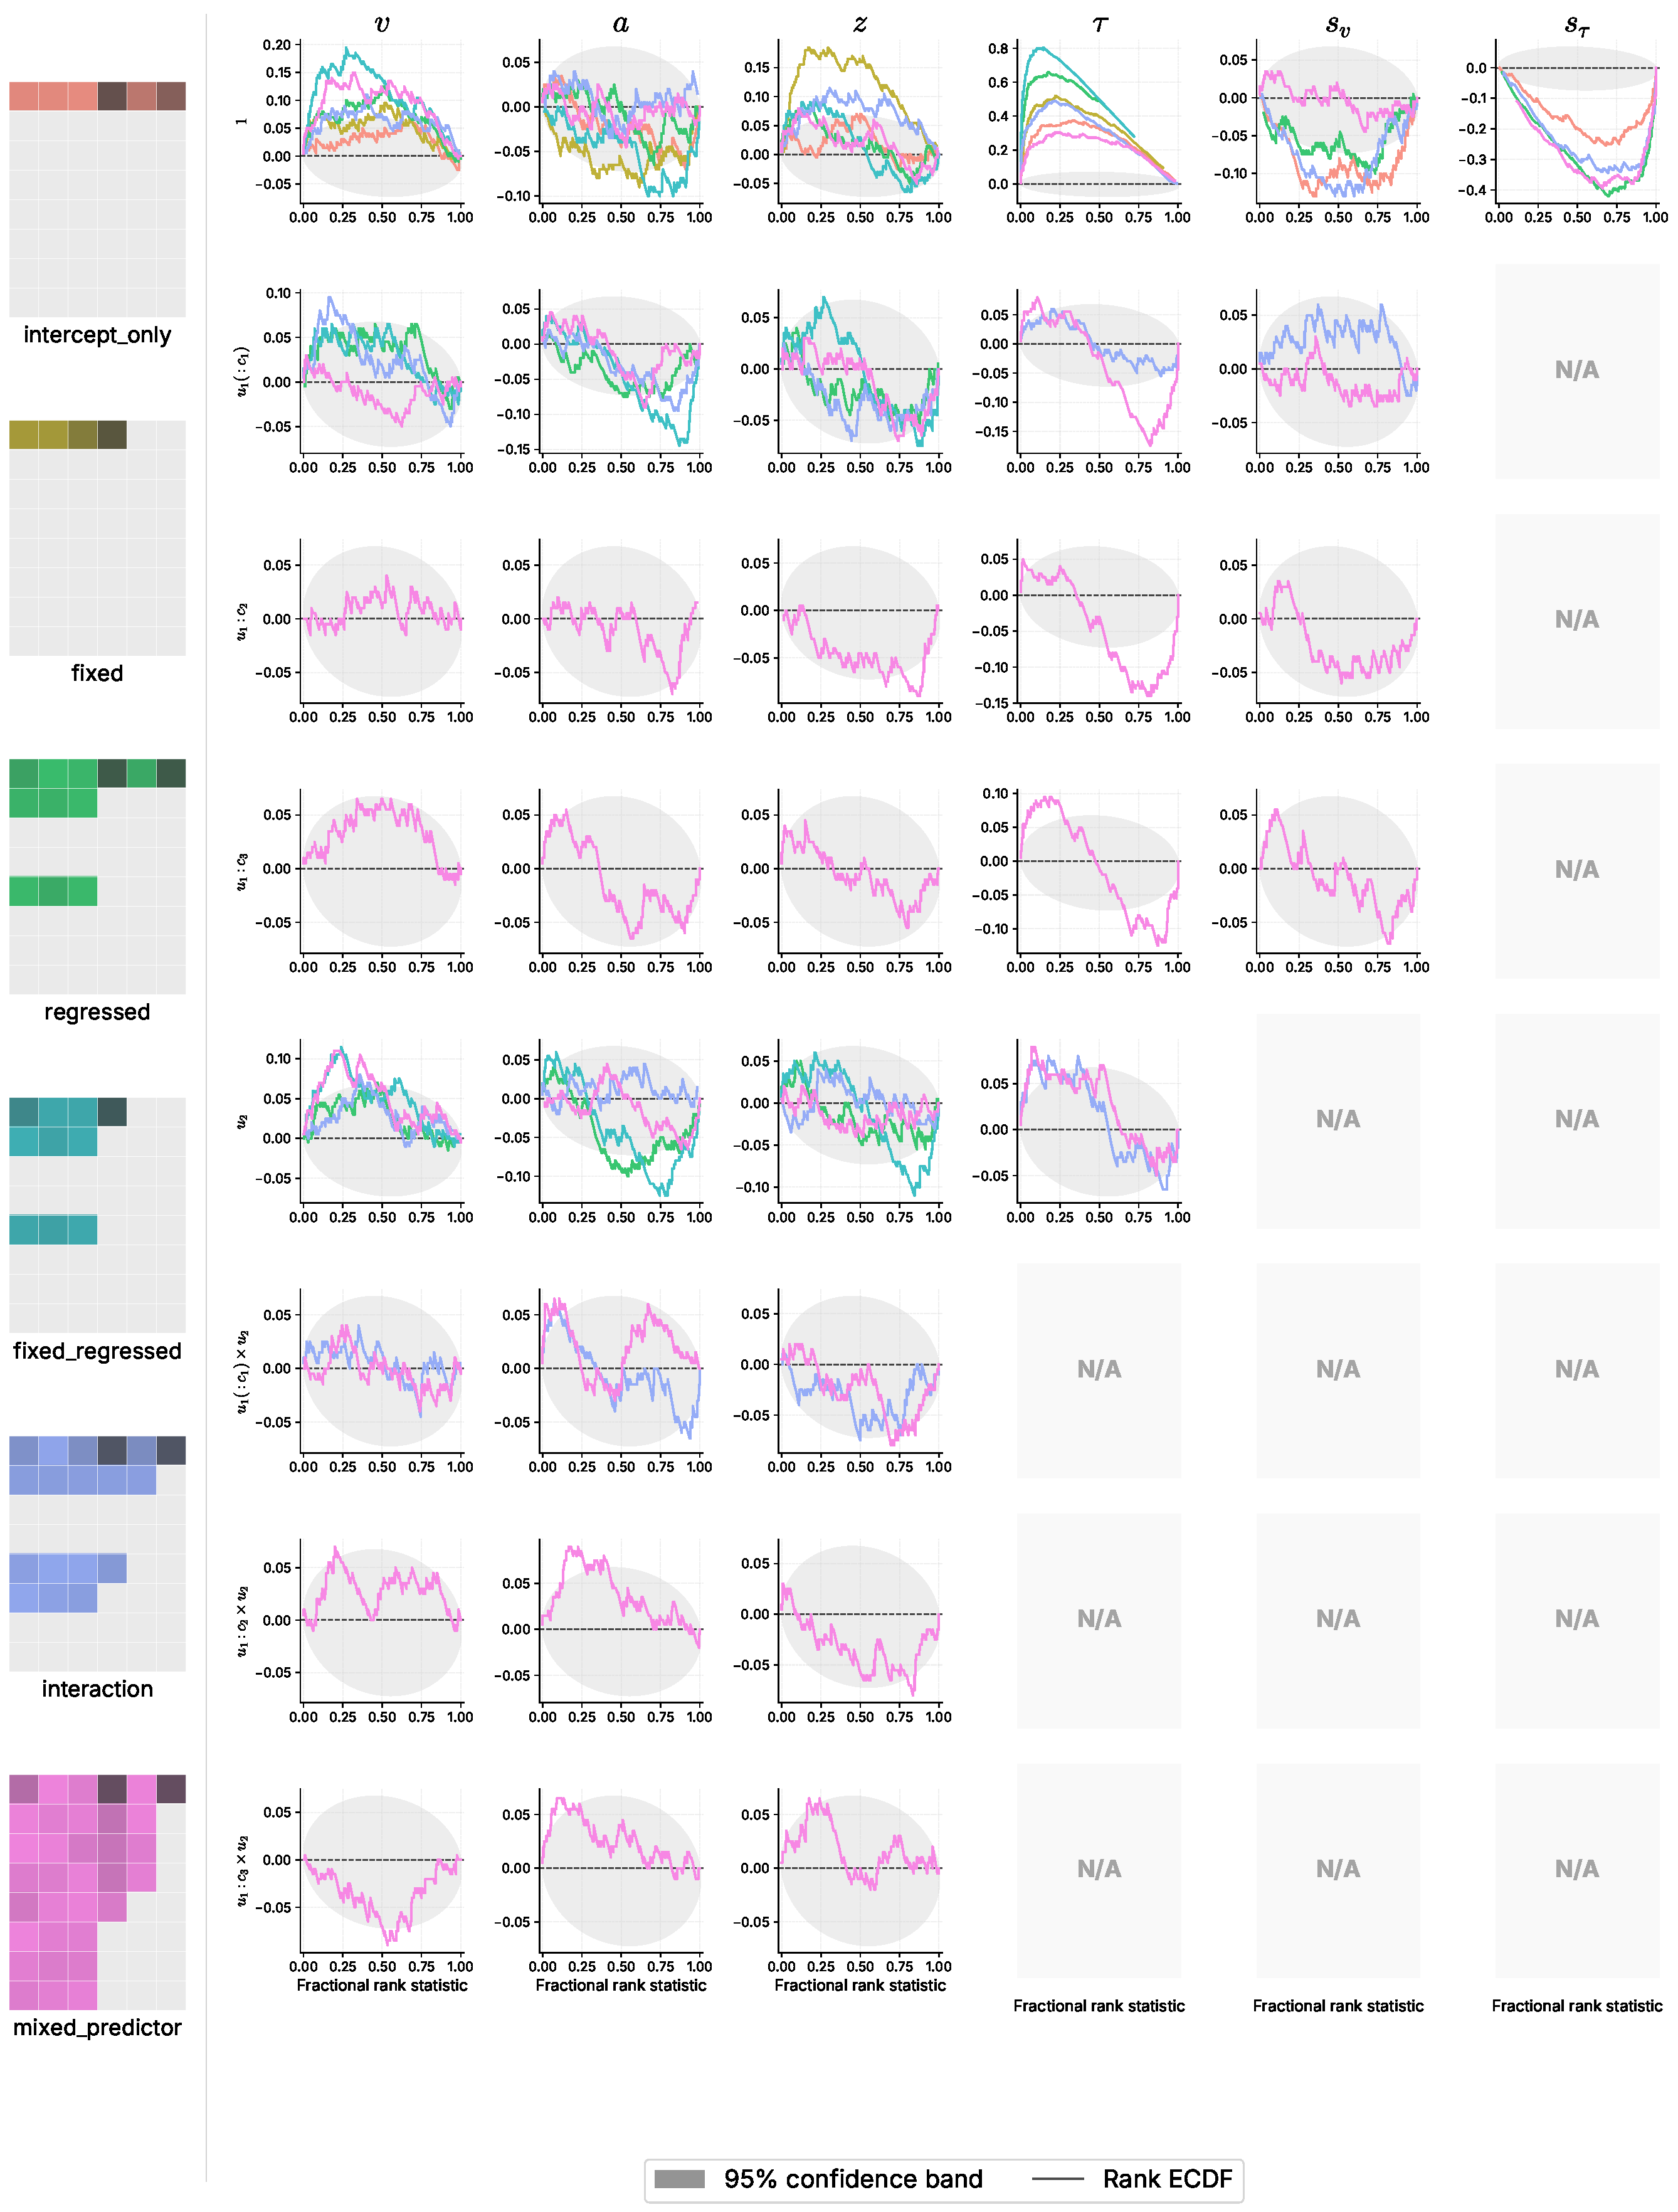
\includegraphics[width=\textwidth,height=0.82\textheight,keepaspectratio]{benchmark_ensemble/bench6/ddm/ecdf.pdf}
  \caption{\textbf{Simulation-based calibration, six-design benchmark ensemble, DDM (CogFormer).} Designs as in Figure~\ref{fig:app1-ddm-bench6-recovery}; encoding as in panel (b) of Figure~\ref{fig:app1-ddm-bench5}.}
  \label{fig:app1-ddm-bench6-ecdf}
\end{figure}

\begin{figure}[p]
  \centering
  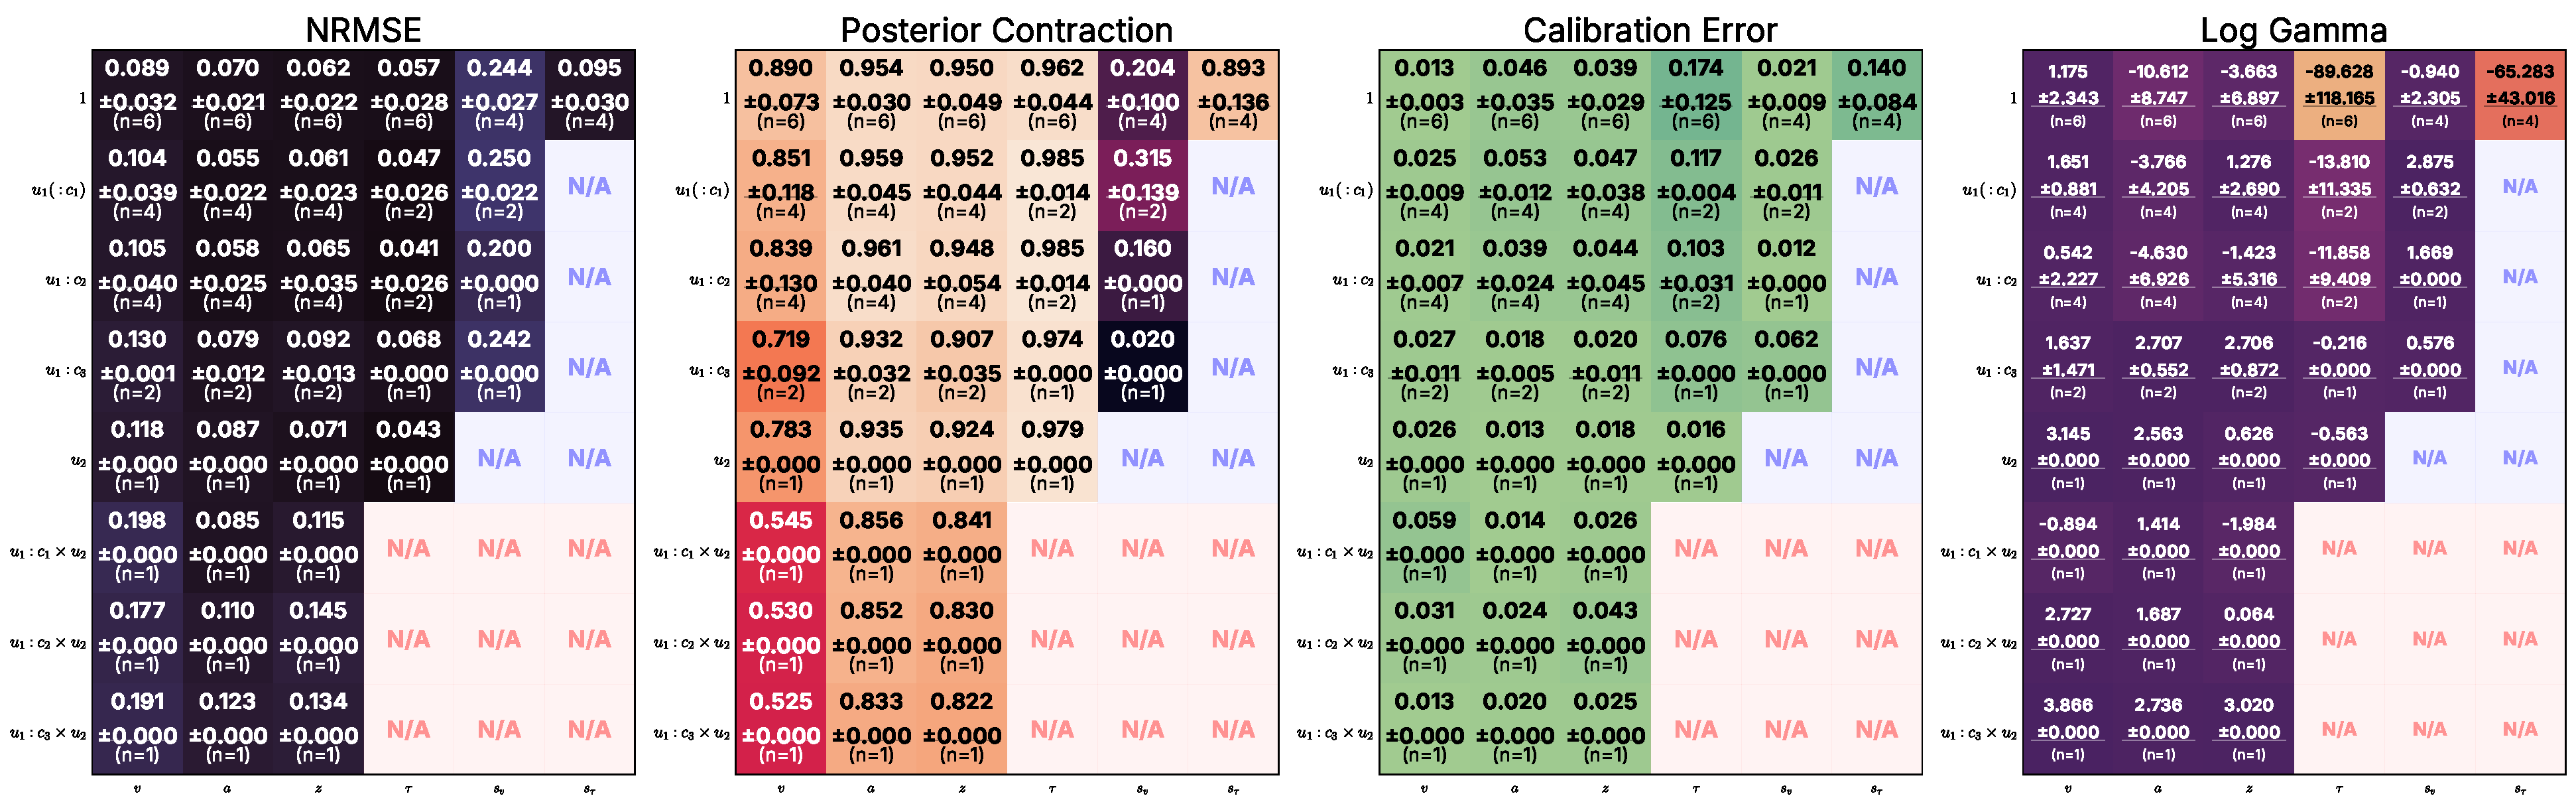
\includegraphics[width=\textwidth,height=0.82\textheight,keepaspectratio]{benchmark_ensemble/bench6/ddm/metrics.pdf}
  \caption{\textbf{Summary metrics, six-design benchmark ensemble, DDM (CogFormer).} Designs as in Figure~\ref{fig:app1-ddm-bench6-recovery}; encoding as in panel (c) of Figure~\ref{fig:app1-ddm-bench5}.}
  \label{fig:app1-ddm-bench6-metrics}
\end{figure}

\begin{figure}[p]
  \centering
  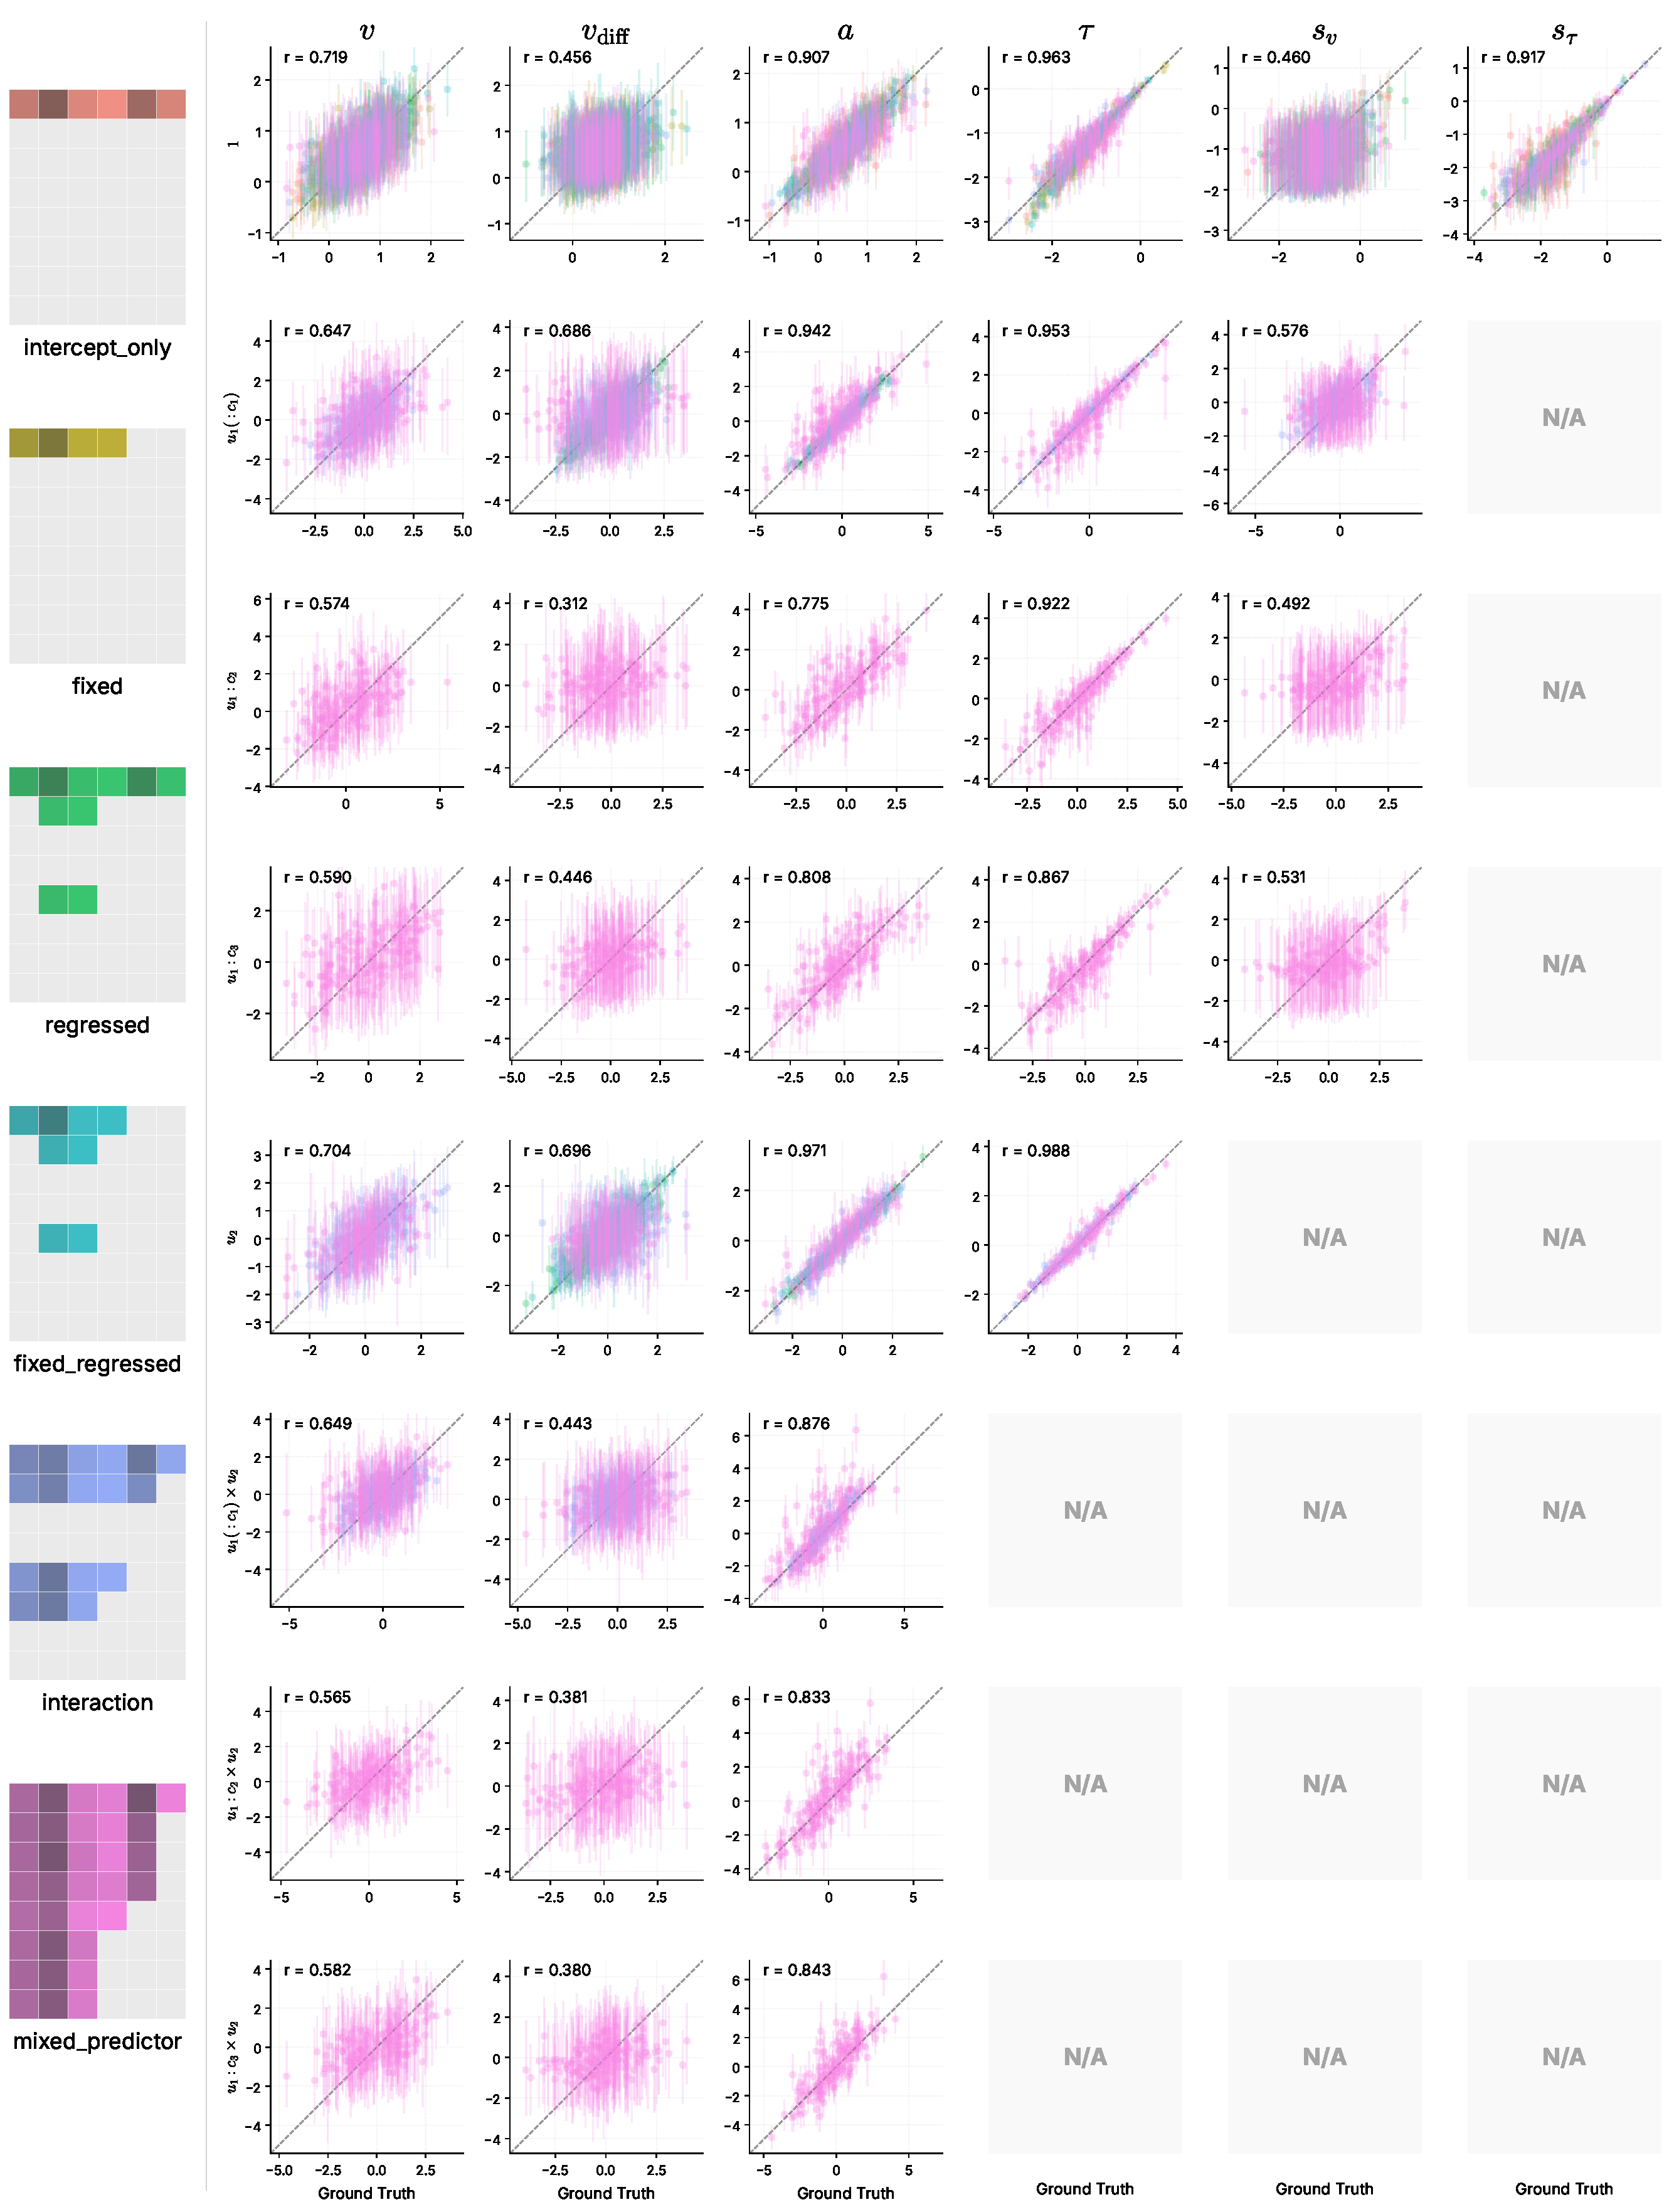
\includegraphics[width=\textwidth,height=0.82\textheight,keepaspectratio]{benchmark_ensemble/bench6/rdm/recovery.pdf}
  \caption{\textbf{Parameter recovery, six-design benchmark ensemble, RDM (CogFormer).} Designs as in Figure~\ref{fig:app1-ddm-bench6-recovery}; encoding as in panel (a) of Figure~\ref{fig:app1-rdm-bench5}.}
  \label{fig:app1-rdm-bench6-recovery}
\end{figure}

\begin{figure}[p]
  \centering
  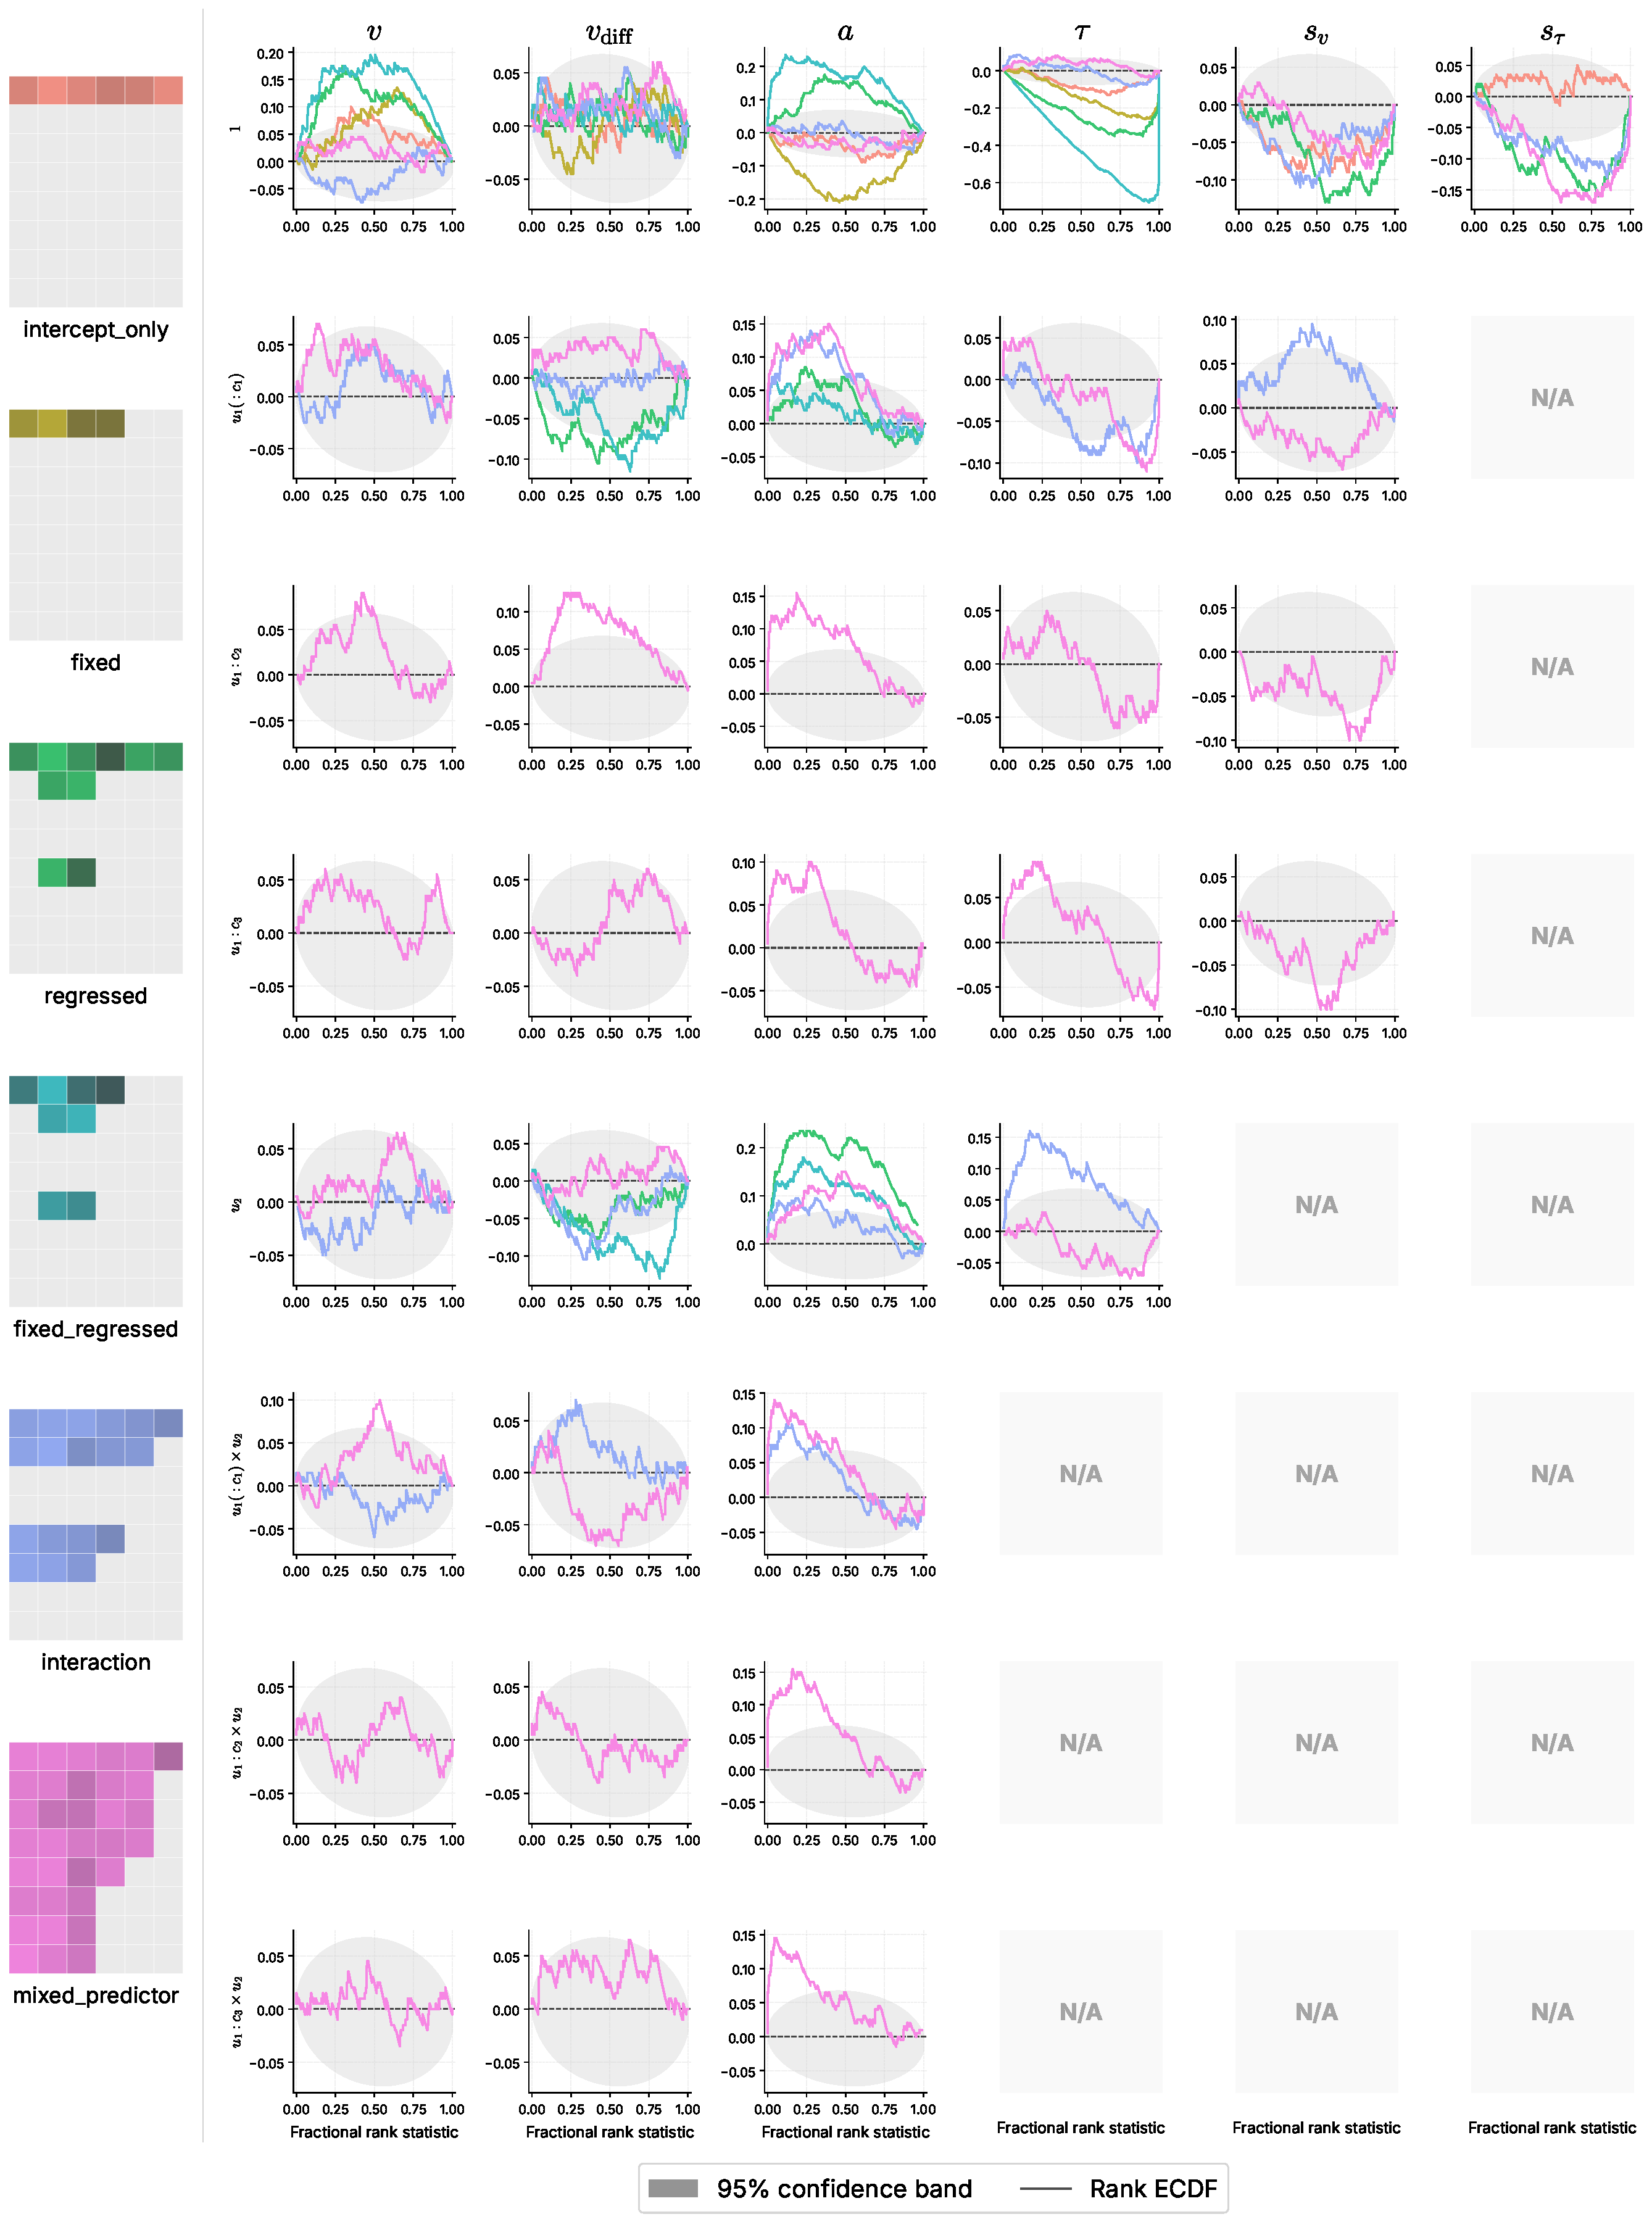
\includegraphics[width=\textwidth,height=0.82\textheight,keepaspectratio]{benchmark_ensemble/bench6/rdm/ecdf.pdf}
  \caption{\textbf{Simulation-based calibration, six-design benchmark ensemble, RDM (CogFormer).} Designs as in Figure~\ref{fig:app1-ddm-bench6-recovery}; encoding as in panel (b) of Figure~\ref{fig:app1-rdm-bench5}.}
  \label{fig:app1-rdm-bench6-ecdf}
\end{figure}

\begin{figure}[p]
  \centering
  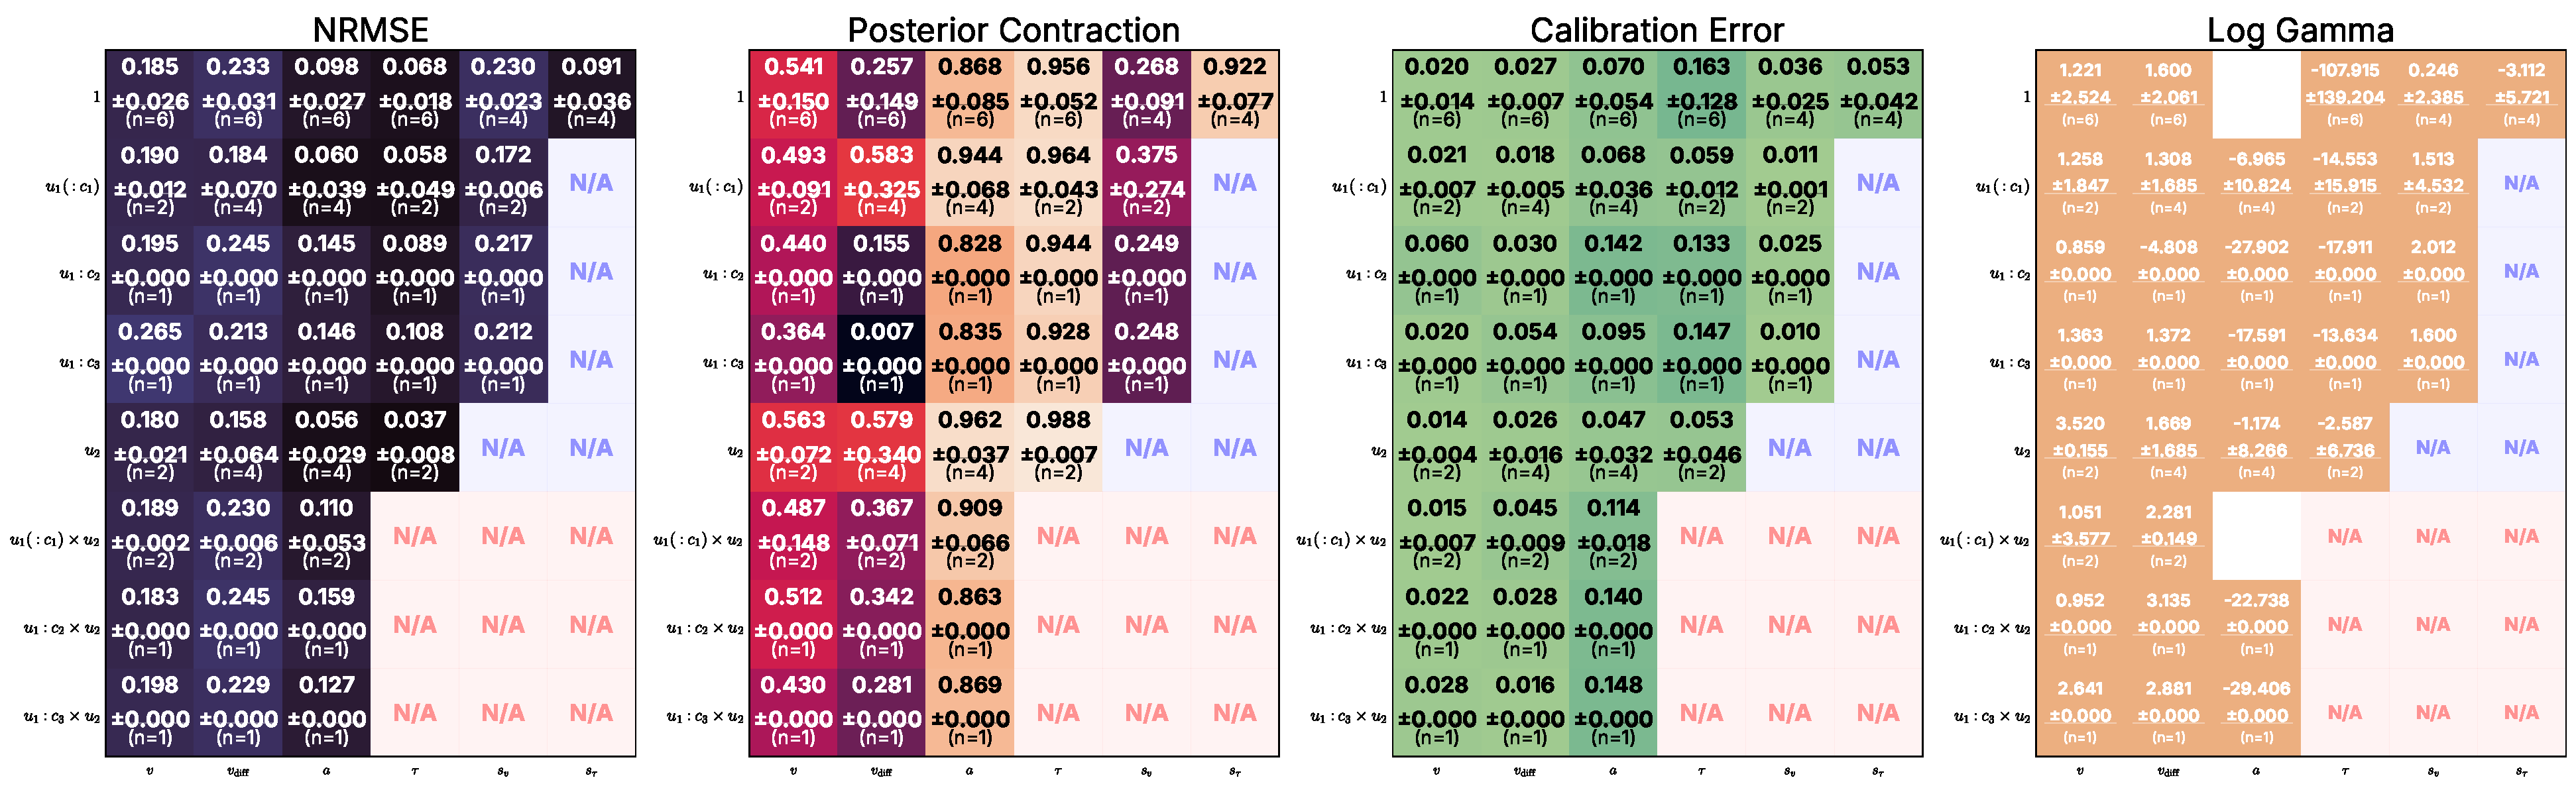
\includegraphics[width=\textwidth,height=0.82\textheight,keepaspectratio]{benchmark_ensemble/bench6/rdm/metrics.pdf}
  \caption{\textbf{Summary metrics, six-design benchmark ensemble, RDM (CogFormer).} Designs as in Figure~\ref{fig:app1-ddm-bench6-recovery}; encoding as in panel (c) of Figure~\ref{fig:app1-rdm-bench5}.}
  \label{fig:app1-rdm-bench6-metrics}
\end{figure}

\begin{figure}[p]
  \centering
  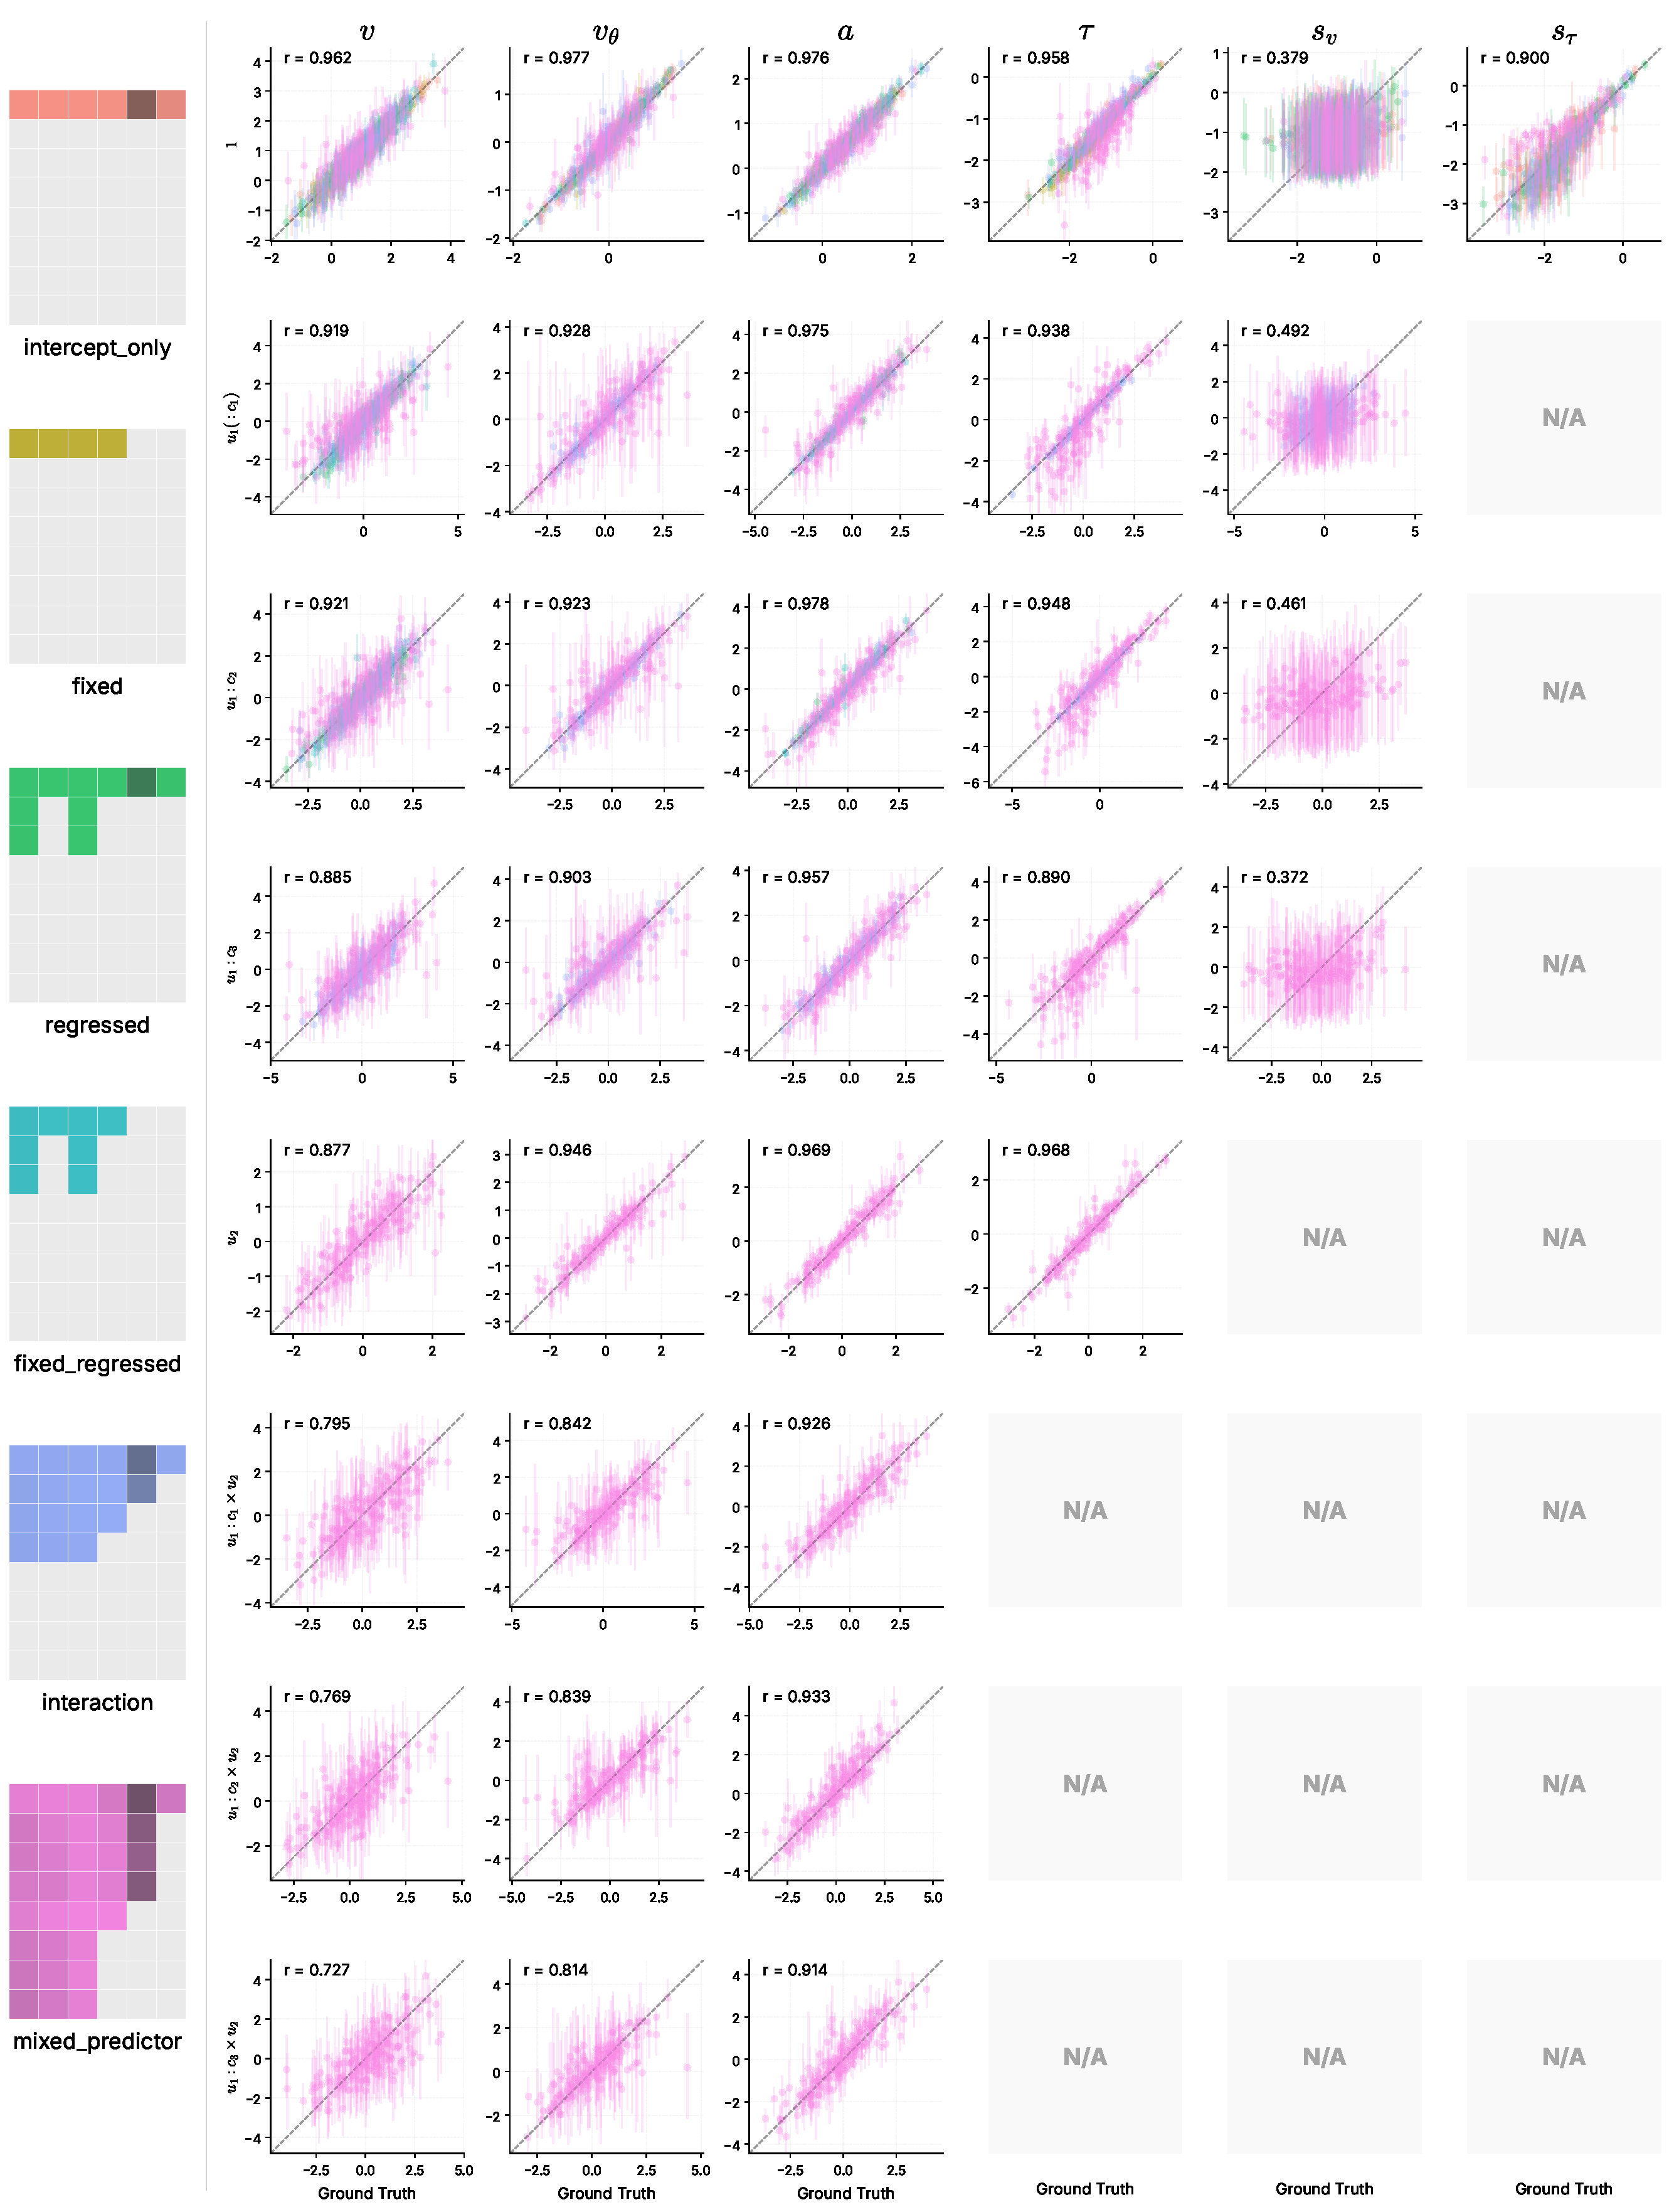
\includegraphics[width=\textwidth,height=0.82\textheight,keepaspectratio]{benchmark_ensemble/bench6/cdm/recovery.pdf}
  \caption{\textbf{Parameter recovery, six-design benchmark ensemble, CDM (CogFormer).} Designs as in Figure~\ref{fig:app1-ddm-bench6-recovery}; encoding as in panel (a) of Figure~\ref{fig:app1-cdm-bench5}.}
  \label{fig:app1-cdm-bench6-recovery}
\end{figure}

\begin{figure}[p]
  \centering
  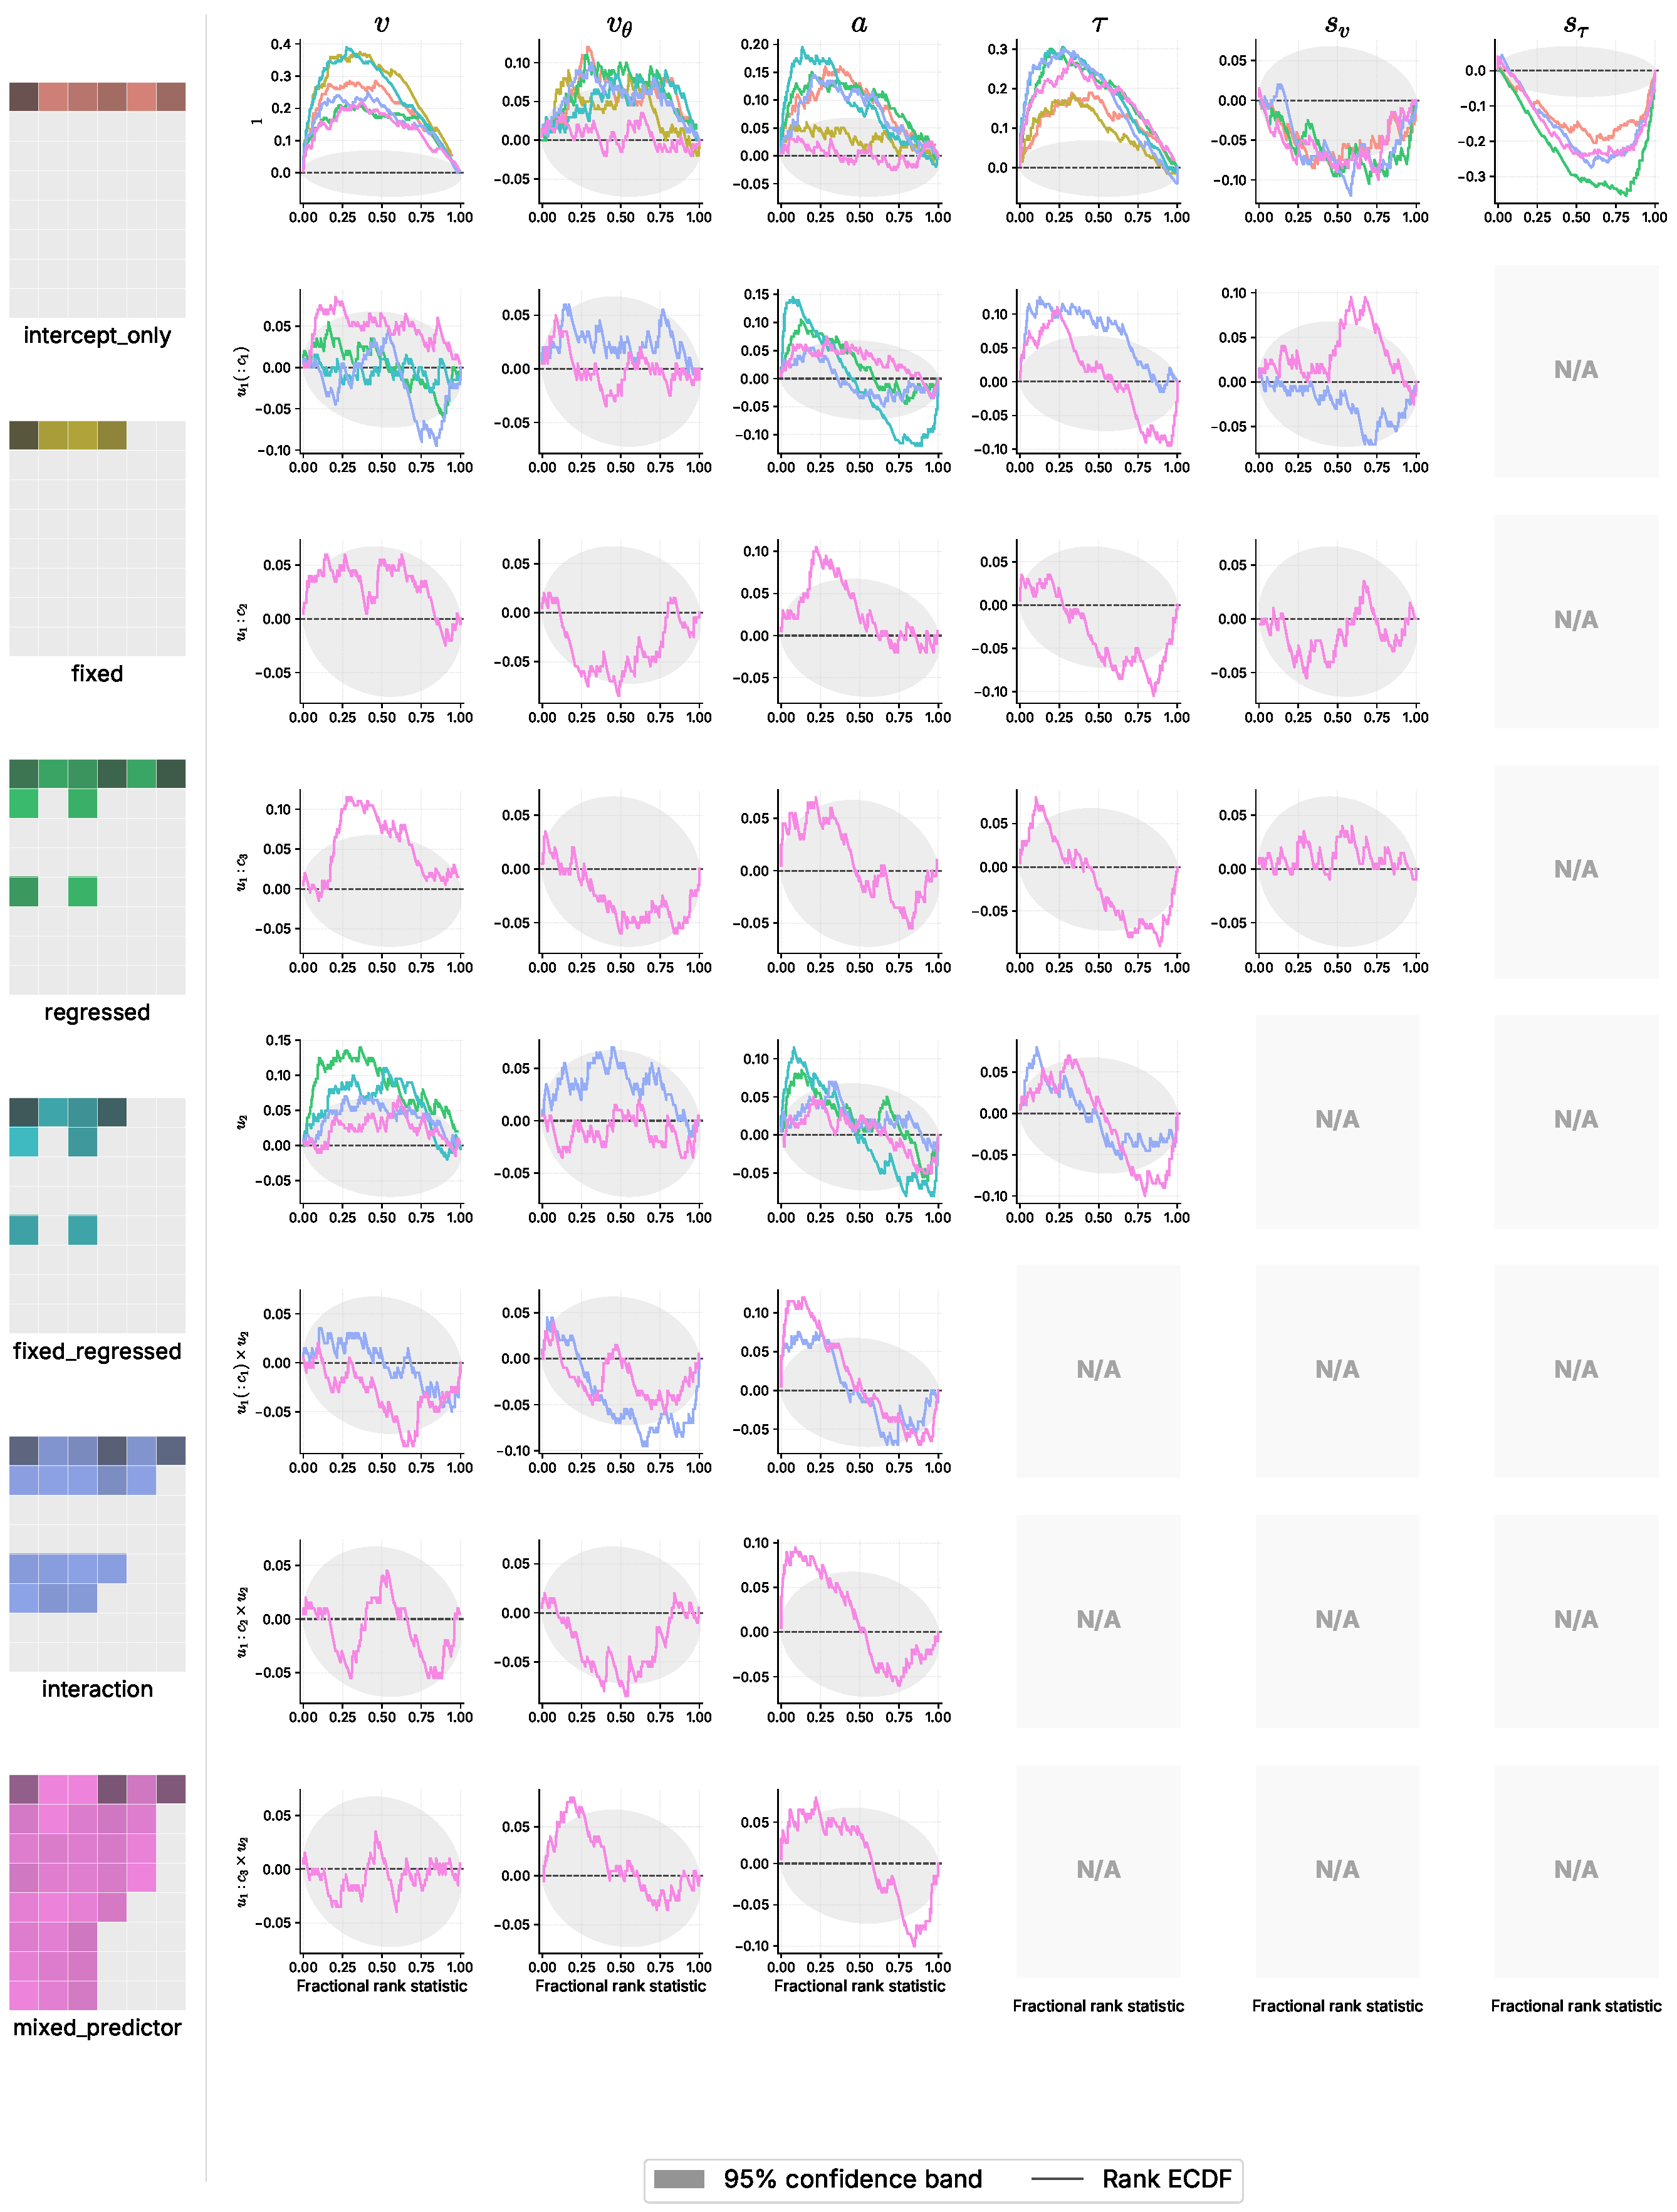
\includegraphics[width=\textwidth,height=0.82\textheight,keepaspectratio]{benchmark_ensemble/bench6/cdm/ecdf.pdf}
  \caption{\textbf{Simulation-based calibration, six-design benchmark ensemble, CDM (CogFormer).} Designs as in Figure~\ref{fig:app1-ddm-bench6-recovery}; encoding as in panel (b) of Figure~\ref{fig:app1-cdm-bench5}.}
  \label{fig:app1-cdm-bench6-ecdf}
\end{figure}

\begin{figure}[p]
  \centering
  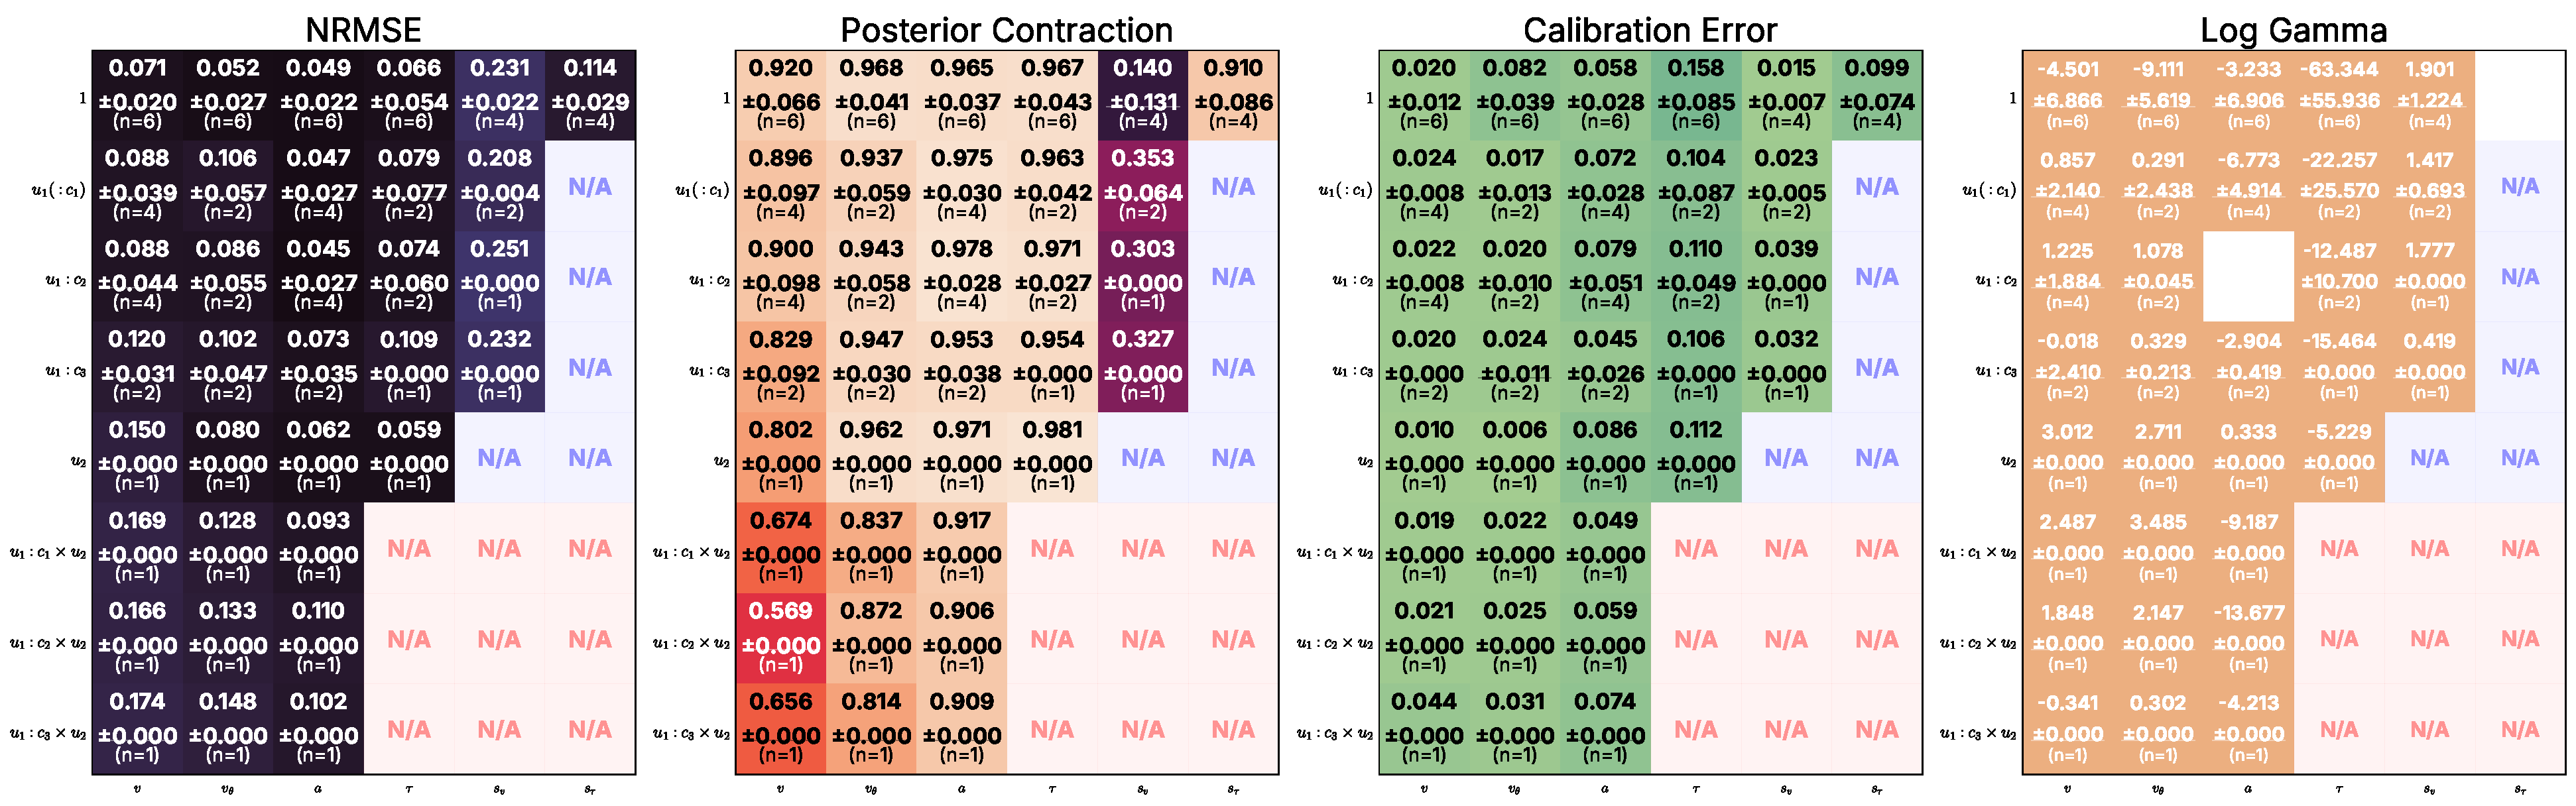
\includegraphics[width=\textwidth,height=0.82\textheight,keepaspectratio]{benchmark_ensemble/bench6/cdm/metrics.pdf}
  \caption{\textbf{Summary metrics, six-design benchmark ensemble, CDM (CogFormer).} Designs as in Figure~\ref{fig:app1-ddm-bench6-recovery}; encoding as in panel (c) of Figure~\ref{fig:app1-cdm-bench5}.}
  \label{fig:app1-cdm-bench6-metrics}
\end{figure}
